\documentclass[german]{../spicker}

\usepackage{amsmath}

\usepackage{graphicx}
\usepackage{tabularx, multirow}
\usepackage{forest}
\usepackage{color, colortbl}

\usetikzlibrary{tikzmark,bbox,calc,automata,arrows.meta,chains,decorations.pathreplacing,scopes,shapes.misc,shapes.multipart}

\definecolor{javared}{rgb}{0.6,0,0} % for strings
\definecolor{javagreen}{rgb}{0.25,0.5,0.35} % comments
\definecolor{javapurple}{rgb}{0.5,0,0.35} % keywords
\definecolor{javadocblue}{rgb}{0.25,0.35,0.75} % javadoc
 
\lstset{language=Java,
basicstyle=\ttfamily,
keywordstyle=\color{javapurple}\bfseries,
stringstyle=\color{javared},
commentstyle=\color{javagreen},
morecomment=[s][\color{javadocblue}]{/**}{*/},
tabsize=4,
showspaces=false,
showstringspaces=false}

\tikzset{
    weight/.style = {
        scale=0.7,
        },
    prim node/.style = {
        fill = blue!50,
        text = white,
        },
    prim edge/.style = {
        draw=blue,
        very thick,
        },
    current/.style = {
        fill = teal!50,
        },
    marked/.style = {
        fill = teal!25,
        },
    visited/.style = {
        fill = teal!30,
        %text=white,
        opacity = 0.5,
    },
    new/.style = {
        red,
    },
    index small/.style = {
        minimum width=1.5em,
        minimum height=0.5em,
        fill = gray!25,
    },
    index/.style = {
        minimum width=2em,
        minimum height=0.5em,
        fill = gray!25,
    },
    every state/.style = {
        minimum size=2em
    }
}

\forestset{%
empty node/.style = {
    dashed,
    opacity = .2, 
    fill opacity = 0.2,
    edge = {opacity=.2},
    },
r/.style = {
    fill = red!50,
    text=white,
    draw=red,
    calign angle=30,
    calign=fixed edge angles,
    %fill opacity = 0.5,
},
b/.style = {
    fill = black!50,
    text=white,
    draw=black,
    calign angle=30,
    calign=fixed edge angles,
    %fill opacity = 0.5,
},
rbn/.style = { %red black not defined
    fill = blue!50,
    text=white,
    draw=black,
    calign angle=30,
    calign=fixed edge angles,
    %fill opacity = 0.5,
},
nil/.style = {
    fill = black!50,
    minimum size=1em,
    calign angle=30,
    calign=fixed edge angles,
    %fill opacity = 0.5,
},
mpn/.style args = {#1/#2/#3/#4}{draw,
rectangle split, rectangle split horizontal,
rectangle split parts=4,
on chain=A,
draw=black!50,
node contents={ \nodepart{one}    $#1$
                \nodepart{two}    $#2$
                \nodepart{three}  $#3$
                \nodepart{four}   $#4$}
                            },
}

\newcommand\mpnc[4]{\nodepart{one}      $#1$
                    \nodepart{two}      $#2$                    
                    \nodepart{three}    $#3$
                    \nodepart{four}     $#4$
                    }

\addbibresource{algo.bib}

\title{Algorithmen}
\author{Patrick Gustav Blaneck}
\makeindex[intoc]
\makeindex[intoc, name=Beispiele,title=Beispiele]

\newenvironment{allintypewriter}{\ttfamily}{\par}

\newcommand{\BF}{\operatorname{BF}} 
\newcommand{\vektor}[1]{\begin{pmatrix*}[c] #1 \end{pmatrix*}}

\pgfmathsetmacro\twopi{2*pi}

\pgfmathdeclarefunction{lngamma}{1}{%
  \pgfmathsetmacro\lngammatmp{#1*#1*#1}%
  \pgfmathparse{%
    #1*ln(#1) - #1 - .5*ln(#1/\twopi)
    + 1/12/#1 - 1/360/\lngammatmp + 1/1260/\lngammatmp/#1/#1
  }%
}  

\pgfmathdeclarefunction{facreal}{1}{%
  \pgfmathparse{exp(lngamma(#1+1))}% 
}

\begin{document}
\maketitle
\tableofcontents
\newpage

\section{Grundbegriffe}
\begin{defi}{Eigenschaften eines Algorithmus}
    \begin{itemize}
        \item \emph{Terminierung:} Der Algorithmus bricht nach \emph{endlichen vielen} Schritten ab.
        \item \emph{Determiniertheit:} Bei vorgegebener Eingabe wird ein eindeutiges \emph{Ergebnis} geliefert.
        \item \emph{Determinismus:} Eindeutige Vorgabe der \emph{Abfolge} der auszuführenden Schritte
    \end{itemize}
\end{defi}

\begin{defi}{Landau-Notation}
    Seien $f, g$ reellwertige Funktionen der reellen Zahlen.
    Dann gilt: \cite{wiki:Landau-Symbole}

    \begin{tabular}{l|l|l}
        Notation          & Definition       & Mathematische Definition                                                                                                  \\
        \hline
        $f \in \bigo(g)$  & obere Schranke   & $\exists C > 0 \exists x_0 > 0 \forall x > x_0 : \abs{f(x)} \leq C \cdot \abs{g(x)}$                                      \\
        $f \in \Omega(g)$ & untere Schranke  & $\exists c > 0 \exists x_0 > 0 \forall x > x_0 : c\cdot \abs{g(x)} \leq \abs{f(x)}$                                       \\
        $f \in \Theta(g)$ & scharfe Schranke & $\exists c > 0 \exists C > 0 \exists x_0 > 0 \forall x > x_0 : c\cdot \abs{g(x)} \leq \abs{f(x)} \leq C \cdot \abs{g(x)}$ \\
    \end{tabular}

    Anschaulicher gilt:

    \begin{tabular}{l|l}
        Notation          & Anschauliche Bedeutung                        \\
        \hline
        $f \in \bigo(g)$  & $f$ wächst nicht wesentlich schneller als $g$ \\
        $f \in \Omega(g)$ & $f$ wächst nicht wesentlich langsamer als $g$ \\
        $f \in \Theta(g)$ & $f$ wächst genauso schnell wie $g$
    \end{tabular}
\end{defi}

\begin{example}{Landau-Notation}
    Aus \cite{wiki:Landau-Symbole} :

    \begin{tabular}{l|l}
        Notation                & Beispiel                                          \\
        \hline
        $f \in \bigo(1)$        & Feststellen, ob eine Binärzahl gerade ist         \\
        $f \in \bigo(\log n)$   & Binäre Suche im sortierten Feld mit $n$ Einträgen \\
        $f \in \bigo(\sqrt{n})$ & Anzahl der Divisionen des naiven Primzahltests    \\
        $f \in \bigo(n)$        & Suche im unsortierten Feld mit $n$ Einträgen      \\
        $f \in \bigo(n\log n)$  & Mergesort, Heapsort                               \\
        $f \in \bigo(n^2)$      & Selectionsort                                     \\
        $f \in \bigo(n^m)$      &                                                   \\
        $f \in \bigo(2^{cn})$   & (Backtracking)                                    \\
        $f \in \bigo(n!)$       & Traveling Salesman Problem
    \end{tabular}
\end{example}

\begin{bonus}{Visualisierung Komplexitätsklassen}
    \begin{center}
        \begin{tikzpicture}[scale=1]
            \begin{axis}[
                    %view={45}{15},
                    width=15cm,
                    unit vector ratio*=1 1,
                    axis lines = middle,
                    grid=major,
                    ymin=0,
                    ymax=50,
                    xmin=0,
                    xmax=50,
                    %zmin=-1,
                    %zmax=10,
                    xlabel = $n$,
                    ylabel = $N$,
                    %zlabel = $z$,
                    %xtick style={draw=none},
                    %ytick style={draw=none},
                    %ztick style={draw=none},
                    xtick distance={5},
                    ytick distance={5},
                    %ztick distance={1},
                    %xticklabels=\empty,
                    %yticklabels=\empty,
                    %zticklabels=\empty,
                    disabledatascaling,
                    %stack dir=minus,
                    cycle list name=color list,
                    samples=250,
                    solid,
                    smooth,
                    line width=1.0pt,
                    no markers,
                    legend cell align={left},
                    reverse legend,
                ]

                \addplot +[domain=0:50]{0};         \addlegendentry{$\bigo(1)$};
                \addplot +[domain=0:50]{ln(x)};     \addlegendentry{$\bigo(\log(n))$};
                \addplot +[domain=0:50]{sqrt(x)};   \addlegendentry{$\bigo(\sqrt{n})$};
                \addplot +[domain=0:50]{x};         \addlegendentry{$\bigo(n)$};
                \addplot +[domain=0:50]{x * ln(x)}; \addlegendentry{$\bigo(n \log(n))$};
                \addplot +[domain=0:50]{x^2};       \addlegendentry{$\bigo(n^2)$};
                \addplot +[domain=0:10]{2^x};        \addlegendentry{$\bigo(2^n)$};
                \addplot +[domain=0:5]{facreal(x)}; \addlegendentry{$\bigo(n!)$};
            \end{axis}
        \end{tikzpicture}
    \end{center}
\end{bonus}


\section{Elementare Datenstrukturen}

% ADTs
\begin{defi}{Abstrakte Datentypen (ADTs)}
    Anforderungen an die Definition eines Datentyps:
    \begin{itemize}
        \item \emph{Spezifikation} eines Datentyps unabhängig von der Implementierung
        \item Reduzierung der von außen sichtbaren Aspekte auf die \emph{Schnittstelle} des Datentyps
    \end{itemize}

    Daraus entstehen \textbf{zwei Prinzipien}:
    \begin{itemize}
        \item \emph{Kapselung:}
              \subitem Zu einem ADT gehört eine Schnittstelle.
              \subitem Zugriffe auf den ADT erfolgen ausschließlich über die Schnittstelle.
        \item \emph{Geheimnisprinzip:}
              \subitem Interne Realisierung eines ADT-Moduls bleibt verborgen.
    \end{itemize}
\end{defi}

\begin{defi}{Homogene Datenstruktur}
    In einer \emph{homogenen Datenstruktur} haben alle Komponenten den \emph{gleichen} Datentyp.
\end{defi}

\begin{defi}{Heterogene Datenstruktur}
    In einer \emph{heterogenen Datenstruktur} haben die Komponenten \emph{unterschiedliche} Datentypen.
\end{defi}

\begin{bonus}{ADTs in Java}
    Viele wichtige abstrakte Datentypen werden in Java durch \emph{Interfaces} beschrieben.

    Es gibt ein oder mehrere Implementierungen dieser Interfaces mit unterschiedlichen dahinter stehenden Konzepten.

    In Java: Package \texttt{java.util}

    Wichtig in der Vorlesung:

    \begin{tabular}{l|l|l}
        ADT                     & Grund-ADT/Interface & Java-Klassen                      \\
        \hline
        Feld                    &                     & (Felder), HashMap                 \\
        Liste                   & List                & ArrayList, LinkedList             \\
        Menge                   & Set                 & HashSet, TreeSet                  \\
        Prioritätswarteschlange &                     & PriorityQueue                     \\
        Stack                   & List                &                                   \\
        Queue                   & List                &                                   \\
        Deque                   & List                & Deque (Interface), ArrayDeque     \\
        Map                     & Set                 & Map (Interface), HashMap, TreeMap \\
        BidiMap                 & Map                 & BidiMap, BiMap (Interface)        \\
        MultiSet, Bag           & Map                 & Bag, Multiset (Interface)
    \end{tabular}
\end{bonus}

\subsection{Abstrakte Datentypen}

\begin{defi}{Array}
    Ein \emph{Array} hat folgende spezielle Eigenschaften:
    \begin{itemize}
        \item Feste Anzahl an Datenobjekten
        \item Auf jedes Objekt kann direkt lesend oder schreibend zugegriffen werden
    \end{itemize}

    \begin{center}
        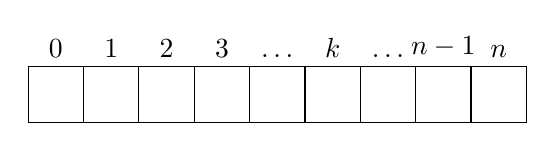
\begin{tikzpicture}[
                %  -{Stealth[length = 2.5pt]},
                start chain,
                node distance = 0pt,
                StackBlock/.style={draw, minimum width=2em, minimum height=2em, outer sep=0pt, on chain},
            ]
            { start chain = going right
                \node [StackBlock, label=$0$] (0) {};
                \node [StackBlock, label=$1$] (1) {};
                \node [StackBlock, label=$2$] (2) {};
                \node [StackBlock, label=$3$] (3) {};
                \node [StackBlock, label=$\ldots$] (d1) {};
                \node [StackBlock, label=$k$] (k) {};
                \node [StackBlock, label=$\ldots$] (d2) {};
                \node [StackBlock, label=$n-1$] (n1) {};
                \node [StackBlock, label=$n$] (n) {};
            }
        \end{tikzpicture}
    \end{center}

    \textbf{Performance:}

    \begin{center}
        \begin{tabular}{c|c|c|c|c}
            Zugriff     & Suche       & Einf./Lösch. (Anfang) & Einf./Lösch. (Ende) & Einf./Lösch. (Mitte) \\
            \hline
            $\Theta(1)$ & $\Theta(n)$ & -                     & -                   & -                    \\
        \end{tabular}
    \end{center}
\end{defi}

\begin{defi}{Liste}
    Eine Liste besteht aus Elementen, die wie in einem Array linear angeordnet sind.
    Auf die Elemente einer Liste muss nicht wahlfrei zugegriffen werden können\footnote{Eine Ausnahme stellt der Listenanfang dar.}.

    Die Größe einer Liste ist nicht von Anfang an bekannt und sie kann beliebig verlängert bzw. verkürzt werden.
\end{defi}

\begin{defi}{Stack}
    \begin{itemize}
        \item Daten können an einem Ende hinzugefügt oder entnommen werden.
    \end{itemize}

    \begin{center}
        \begin{tikzpicture}[
                %  -{Stealth[length = 2.5pt]},
                start chain,
                node distance = 0pt,
                StackBlock/.style={draw, minimum width=2em, minimum height=2em, outer sep=0pt, on chain},
            ]
            { start chain = going right
                \node [StackBlock,draw=none] (0) {};

                \node [StackBlock,xshift=4em] (1) {};
                \node [StackBlock] (2) {};
                \node [StackBlock] (3) {};
                \node [StackBlock] (4) {};
                \node [StackBlock] (5) {};

                \node [StackBlock,xshift=4em,draw=none] (6) {};

                \draw[->] ([yshift=0.5em, xshift=0.25em] 5.east) [out=0, in=180] to ([yshift=0.5em, xshift=-0.25em] 6.west);
                \draw[->] ([yshift=-0.5em, xshift=-0.25em] 6.west) [out=180, in=0] to ([yshift=-0.5em, xshift=0.25em] 5.east);
            }
        \end{tikzpicture}
    \end{center}
\end{defi}

\begin{defi}{Queue}
    \begin{itemize}
        \item Daten können an einem Ende hinzugefügt und am anderen Ende entnommen werden.
    \end{itemize}

    \begin{center}
        \begin{tikzpicture}[
                %  -{Stealth[length = 2.5pt]},
                start chain,
                node distance = 0pt,
                StackBlock/.style={draw, minimum width=2em, minimum height=2em, outer sep=0pt, on chain},
            ]
            { start chain = going right
                \node [StackBlock,draw=none] (0) {};

                \node [StackBlock,xshift=4em] (1) {};
                \node [StackBlock] (2) {};
                \node [StackBlock] (3) {};
                \node [StackBlock] (4) {};
                \node [StackBlock] (5) {};

                \node [StackBlock,xshift=4em,draw=none] (6) {};

                \draw[<-] ([xshift=0.25em] 0.east) [out=0, in=180] to ([xshift=-0.25em] 1.west);
                \draw[->] ([xshift=-0.25em] 6.west) [out=180, in=0] to ([xshift=0.25em] 5.east);
            }
        \end{tikzpicture}
    \end{center}
\end{defi}

\begin{defi}{Deque (\glqq Double ended queue\grqq)}
    \begin{itemize}
        \item Daten können an beiden Enden hinzugefügt und entnommen werden.
    \end{itemize}

    \begin{center}
        \begin{tikzpicture}[
                %  -{Stealth[length = 2.5pt]},
                start chain,
                node distance = 0pt,
                StackBlock/.style={draw, minimum width=2em, minimum height=2em, outer sep=0pt, on chain},
            ]
            { start chain = going right
                \node [StackBlock,draw=none] (0) {};

                \node [StackBlock,xshift=4em] (1) {};
                \node [StackBlock] (2) {};
                \node [StackBlock] (3) {};
                \node [StackBlock] (4) {};
                \node [StackBlock] (5) {};

                \node [StackBlock,xshift=4em,draw=none] (6) {};

                \draw[->] ([yshift=0.5em, xshift=0.25em] 5.east) [out=0, in=180] to ([yshift=0.5em, xshift=-0.25em] 6.west);
                \draw[->] ([yshift=-0.5em, xshift=-0.25em] 6.west) [out=180, in=0] to ([yshift=-0.5em, xshift=0.25em] 5.east);

                \draw[<-] ([yshift=0.5em, xshift=0.25em] 0.east) [out=0, in=180] to ([yshift=0.5em, xshift=-0.25em] 1.west);
                \draw[<-] ([yshift=-0.5em, xshift=-0.25em] 1.west) [out=180, in=0] to ([yshift=-0.5em, xshift=0.25em] 0.east);
            }
        \end{tikzpicture}
    \end{center}
\end{defi}

\begin{bonus}{Prioritätswarteschlange}
    Eine \emph{Prioritätswarteschlange} ist eine Warteschlange, deren Elemente einen Schlüssel (\emph{Priorität}) besitzen.

    \textbf{Implementierung:}

    In Java dient zur Implementierung die Klasse \texttt{PriorityQueue}, alternativ auch \texttt{TreeSet}.
\end{bonus}

% Mengen
\begin{defi}{Menge}
    Eine \emph{Menge (Set)} ist eine Sammlung von Elementen des gleichen Datentyps.
    Innerhalb der Menge sind die Elemente ungeordnet.
    Jedes Element kann nur einmal in der Menge vorkommen.

    \textbf{Implementierung:}

    In Java ist \emph{Set} ein Interface, das unter anderem folgende Klassen implementiert:
    \begin{itemize}
        \item \texttt{TreeSet}: Basiert auf der Datenstruktur Rot-Schwarz-Baum, implementiert Erweiterung \texttt{SortedMap}.
        \item \texttt{HashSet}: Basiert auf der Datenstruktur Hashtabelle.
    \end{itemize}
\end{defi}

% Assoziative Felder
\begin{defi}{Assoziatives Feld}
    Ein \emph{assoziatives Feld} ist eine Sonderform des Feldes:
    \begin{itemize}
        \item Verwendet keinen numerischen Index zur Adressierung eines Elements.
        \item Verwendet zur Adressierung einen Schlüssel (z.B. \texttt{a["Meier"]}).
    \end{itemize}

    Assoziative Felder eignen sich dazu, Datenelemente in einer großen Datenmenge aufzufinden.
    Jedes Datenelement wird durch einen \emph{eindeutigen Schlüssel} identifiziert.

    \textbf{Implementierung:}

    In Java entspricht ein \emph{assoziatives Feld} dem Interface \texttt{java.util.Map}, das folgende Klassen implementiert:
    \begin{itemize}
        \item \texttt{TreeMap}: Basiert auf der Datenstruktur Rot-Schwarz-Baum, implementiert Erweiterung \texttt{SortedMap}.
        \item \texttt{HashMap}: Basiert auf der Datenstruktur Hashtabelle.
    \end{itemize}
\end{defi}

\subsection{Datenstrukturen}
% Listen
\begin{defi}{Einfach verkettete Liste}
    Im Vergleich zu einem Array kann eine \emph{Liste} schrumpfen und wachsen.

    \begin{center}
        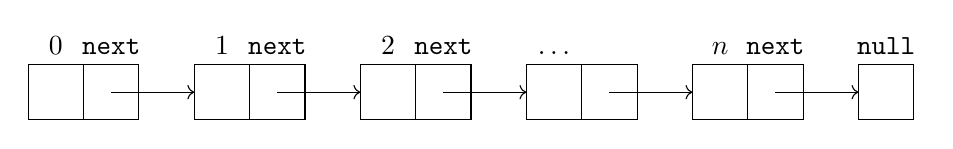
\begin{tikzpicture}[
                %  -{Stealth[length = 2.5pt]},
                start chain,
                node distance = 0pt,
                StackBlock/.style={draw, minimum width=2em, minimum height=2em, outer sep=0pt, on chain},
            ]
            { start chain = going right
                \node [StackBlock, label=$0$] (0) {};
                \node [StackBlock, label=\texttt{next}] (0p) {};
                \node [StackBlock, label=$1$,xshift=2em] (1) {};
                \node [StackBlock, label=\texttt{next}] (1p) {};
                \node [StackBlock, label=$2$,xshift=2em] (2) {};
                \node [StackBlock, label=\texttt{next}] (2p) {};
                \node [StackBlock, label=$\ldots$,xshift=2em] (dots) {};
                \node [StackBlock] (dotsp) {};
                \node [StackBlock, label=$n$,xshift=2em] (n) {};
                \node [StackBlock, label=\texttt{next}] (np) {};
                \node [StackBlock, label=\texttt{null}, xshift=2em] (null) {};


                \draw[->] (0p.center) [out=0, in=180] to (1.west);
                \draw[->] (1p.center) [out=0, in=180] to (2.west);
                \draw[->] (2p.center) [out=0, in=180] to (dots.west);
                \draw[->] (dotsp.center) [out=0, in=180] to (n.west);
                \draw[->] (np.center) [out=0, in=180] to (null.west);
            }
        \end{tikzpicture}
    \end{center}

    \textbf{Performance:}

    \begin{center}
        \begin{tabular}{c|c|c|c|c}
            Zugriff     & Suche       & Einf./Lösch. (Anfang) & Einf./Lösch. (Ende)                                                                                 & Einf./Lösch. (Mitte)   \\
            \hline
            $\Theta(n)$ & $\Theta(n)$ & $\Theta(1)$           & $\Theta(1)/\Theta(n)$\footnote{$\Theta(1)$, wenn das letzte Element bekannt ist, $\Theta(n)$ sonst} & Suchzeit + $\Theta(1)$ \\
        \end{tabular}
    \end{center}
\end{defi}


\begin{defi}{Doppelt verkettete Liste}
    Im Vergleich zu einer einfach verketteten Liste besitzt die \emph{doppelt verkettete Liste} zusätzlich einen Verweis auf den Vorgänger.

    \begin{center}
        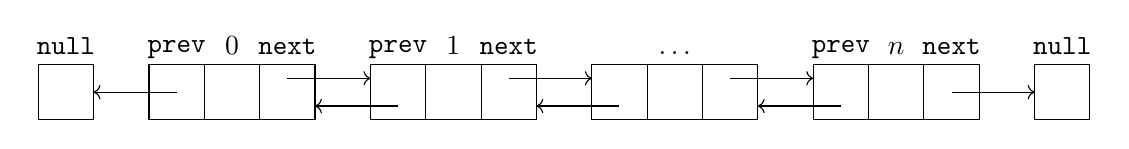
\begin{tikzpicture}[
                %  -{Stealth[length = 2.5pt]},
                start chain,
                node distance = 0pt,
                StackBlock/.style={draw, minimum width=2em, minimum height=2em, outer sep=0pt, on chain},
            ]
            { start chain = going right
                \node [StackBlock,label=\texttt{null}] (nulll) {};

                \node [StackBlock,label={[label distance=-.35ex]above:\texttt{prev}}, xshift=2em] (0p) {};
                \node [StackBlock,label=$0$] (0) {};
                \node [StackBlock,label=\texttt{next}] (0n) {};
                \node [StackBlock,label={[label distance=-.35ex]above:\texttt{prev}},xshift=2em] (1p) {};
                \node [StackBlock,label=$1$] (1) {};
                \node [StackBlock,label=\texttt{next}] (1n) {};
                \node [StackBlock,xshift=2em] (dotsp) {};
                \node [StackBlock,label=$\ldots$] (dots) {};
                \node [StackBlock] (dotsn) {};
                \node [StackBlock,label={[label distance=-.35ex]above:\texttt{prev}},xshift=2em] (np) {};
                \node [StackBlock,label=$n$] (n) {};
                \node [StackBlock,label=\texttt{next}] (nn) {};

                \node [StackBlock,label=\texttt{null}, xshift=2em] (nullr) {};

                %\draw[->] ([yshift=0.5em, xshift=0.25em] 5.east) [out=0, in=180] to ([yshift=0.5em, xshift=-0.25em] 6.west);

                % next arrows
                \draw[->] ([yshift=0.5em] 0n.center) [out=0, in=180] to ([yshift=0.5em] 1p.west);
                \draw[->] ([yshift=0.5em] 1n.center) [out=0, in=180] to ([yshift=0.5em] dotsp.west);
                \draw[->] ([yshift=0.5em] dotsn.center) [out=0, in=180] to ([yshift=0.5em] np.west);

                \draw[->] (nn.center) [out=0, in=180] to (nullr.west);

                % prev arrows
                \draw[<-] ([yshift=-0.5em] 0n.east) [out=0, in=180] to ([yshift=-0.5em] 1p.center);
                \draw[<-] ([yshift=-0.5em] 1n.east) [out=0, in=180] to ([yshift=-0.5em] dotsp.center);
                \draw[<-] ([yshift=-0.5em] dotsn.east) [out=0, in=180] to ([yshift=-0.5em] np.center);

                \draw[->] (0p.center) [out=180, in=0] to (nulll.east);
            }
        \end{tikzpicture}
    \end{center}

    \textbf{Performance:}

    \begin{center}
        \begin{tabular}{c|c|c|c|c}
            Zugriff     & Suche       & Einf./Lösch. (Anfang) & Einf./Lösch. (Ende) & Einf./Lösch. (Mitte)   \\
            \hline
            $\Theta(n)$ & $\Theta(n)$ & $\Theta(1)$           & $\Theta(1)$         & Suchzeit + $\Theta(1)$ \\
        \end{tabular}
    \end{center}
\end{defi}

% Dynamische Felder
\begin{defi}{Dynamisches Feld}
    Ein \emph{dynamisches Feld} besteht aus:
    \begin{itemize}
        \item Einem normalen Feld, das nicht vollständig gefüllt ist.
        \item Einem Zeiger, der anzeigt, welches das erste unbesetzte Element ist.
    \end{itemize}

    \begin{center}
        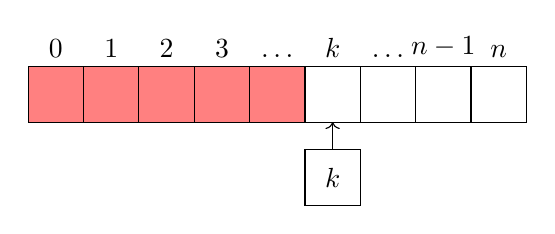
\begin{tikzpicture}[
            %  -{Stealth[length = 2.5pt]},
            start chain,
            node distance = 0pt,
            StackBlock/.style={draw, minimum width=2em, minimum height=2em, outer sep=0pt, on chain},
            ]
            { start chain = going right
            \node [StackBlock, fill=red!50, label=$0$] (0) {};
            \node [StackBlock, fill=red!50, label=$1$] (1) {};
            \node [StackBlock, fill=red!50, label=$2$] (2) {};
            \node [StackBlock, fill=red!50, label=$3$] (3) {};
            \node [StackBlock, fill=red!50, label=$\ldots$] (d1) {};
            \node [StackBlock, label=$k$] (k) {};
            \node [StackBlock, label=$\ldots$] (d2) {};
            \node [StackBlock, label=$n-1$] (n1) {};
            \node [StackBlock, label=$n$] (n) {};

            { [continue chain = going below]
            \chainin (k);
            \node[StackBlock,yshift=-1em] (pointer) {$k$};
            \draw[->] (pointer.north) [out=90, in=-90] to (k.south);
            }

            }
            %\begin{scope}[-{Stealth[length = 2.5pt]}]
            %\draw (1.north) [out=25, in=155] to (2.north);
            %\draw (1.north) [out=30, in=155] to (3.north);
            %\draw (1.north) [out=35, in=155] to (4.north);
            %\draw (6.north) [out=40, in=155] to (6.north);
            %\end{scope}
            %\draw[decorate,decoration={brace, amplitude=10pt, raise=5pt, mirror}]
            %(2.south west) to node[black,midway,below= 15pt] {$k$-elements} (7.south east);%

        \end{tikzpicture}
    \end{center}

    \textbf{Performance:}

    \begin{center}
        \begin{tabular}{c|c|c|c|c}
            Zugriff     & Suche       & Einf./Lösch. (Anfang) & Einf./Lösch. (Ende)                                                                                     & Einf./Lösch. (Mitte) \\
            \hline
            $\Theta(1)$ & $\Theta(n)$ & $\Theta(n)$           & $\Theta(1)/\Theta(n)$\footnote{Wenn das Feld schon voll ist, muss der komplette Inhalt kopiert werden.} & $\Theta(n)$          \\
        \end{tabular}
    \end{center}

    Damit ist ein dynamisches Feld gut für einen \emph{Stack} geeignet!
\end{defi}

% Zirkuläre dynamische Felder
\begin{defi}{Zirkuläres (dynamisches) Feld}
    Ein \emph{zirkuläres Feld} besitzt einen Speicher fester Größe.
    Dabei speichern zwei Zeiger jeweils den Anfang (\texttt{head}) des Speichers, bzw. auf die nächste freie Speicheradresse (\texttt{tail}) im Speicher.

    Wird ein Element am Anfang \glqq abgearbeitet\grqq, bewegt sich \texttt{head} eine Position weiter.
    Wird ein Element am Ende eingefügt, bewegt sich \texttt{tail} eine Position weiter.
    \begin{center}
        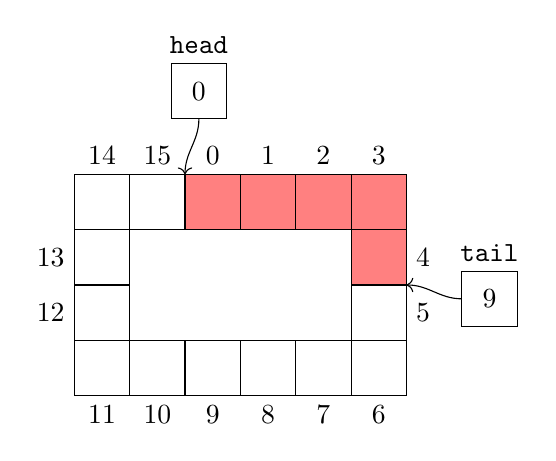
\begin{tikzpicture}[
            %  -{Stealth[length = 2.5pt]},
            start chain,
            node distance = 0pt,
            StackBlock/.style={draw, minimum width=2em, minimum height=2em, outer sep=0pt, on chain},
            ]
            { start chain = going right
            \node [StackBlock,label=above:$15$] (15) {};
            \node [StackBlock,label=above:$0$, fill=red!50] (0) {};
            \node [StackBlock,label=above:$1$, fill=red!50] (1) {};
            \node [StackBlock,label=above:$2$, fill=red!50] (2) {};
            \node [StackBlock,label=above:$3$, fill=red!50] (3) {};

            { [continue chain = going below]
            \chainin (3);
            \node [StackBlock,label=right:$4$, fill=red!50] (4) {};
            \node [StackBlock,label=right:$5$] (5) {};
            \node [StackBlock,label=below:$6$] (6) {};
            }

            { [continue chain = going left]
            \chainin (6);
            \node [StackBlock,label=below:$7$] (7) {};
            \node [StackBlock,label=below:$8$] (8) {};
            \node [StackBlock,label=below:$9$] (9) {};
            \node [StackBlock,label=below:$10$] (10) {};
            \node [StackBlock,label=below:$11$] (11) {};
            }

            { [continue chain = going above]
            \chainin (11);
            \node [StackBlock,label=left:$12$] (12) {};
            \node [StackBlock,label=left:$13$] (13) {};
            \node [StackBlock,label=above:$14$] (14) {};
            }


            { [continue chain = going above]
            \chainin (0);
            \node[StackBlock,yshift=2em,xshift=-0.5em,label=\texttt{head}] (head) {$0$};
            \draw[->] (head.south) [out=-90, in=90] to (0.north west);
            }

            { [continue chain = going right]
            \chainin (5);
            \node[StackBlock,yshift=0.5em,xshift=2em,label=above:\texttt{tail}] (tail) {$9$};
            \draw[->] (tail.west) [out=180, in=0] to (5.north east);
            }
            }
            %\begin{scope}[-{Stealth[length = 2.5pt]}]
            %\draw (1.north) [out=25, in=155] to (2.north);
            %\draw (1.north) [out=30, in=155] to (3.north);
            %\draw (1.north) [out=35, in=155] to (4.north);
            %\draw (6.north) [out=40, in=155] to (6.north);
            %\end{scope}
            %\draw[decorate,decoration={brace, amplitude=10pt, raise=5pt, mirror}]
            %(2.south west) to node[black,midway,below= 15pt] {$k$-elements} (7.south east);%

        \end{tikzpicture}
    \end{center}

    \textbf{Performance:} (dynamisch, bei unterliegender Datenstruktur Array)

    \begin{center}
        \begin{tabular}{c|c|c|c|c}
            Zugriff     & Suche       & Einf./Lösch. (Anfang)                                                                                   & Einf./Lösch. (Ende)                              & Einf./Lösch. (Mitte) \\
            \hline
            $\Theta(1)$ & $\Theta(n)$ & $\Theta(1)/\Theta(n)$\footnote{Wenn das Feld schon voll ist, muss der komplette Inhalt kopiert werden.} & $\Theta(1)/\Theta(n)$\footnote{Siehe Fußnote a.} & $\Theta(n)$          \\
        \end{tabular}
    \end{center}

    Damit ist ein zirkuläres (dynamisches) Feld gut für eine \emph{Queue/Deque} geeignet!
\end{defi}

% Verkettete Listen

\subsection{Hashing}

% Hashtabellen

\begin{defi}{Hashfunktion}
    Eine Hashfunktion oder Streuwertfunktion ist eine Abbildung $h : S \to I$, die eine große Eingabemenge, die Schlüssel $S$, auf eine kleinere Zielmenge, die Hashwerte $I$, abbildet.\footnote{Eine Hashfunktion ist daher im Allgemeinen nicht injektiv, aber surjektiv.}

    Die Bildmenge $h(S) \subseteq I$ bezeichnet die Menge der \emph{Hash-Indizes}.


    \begin{center}
        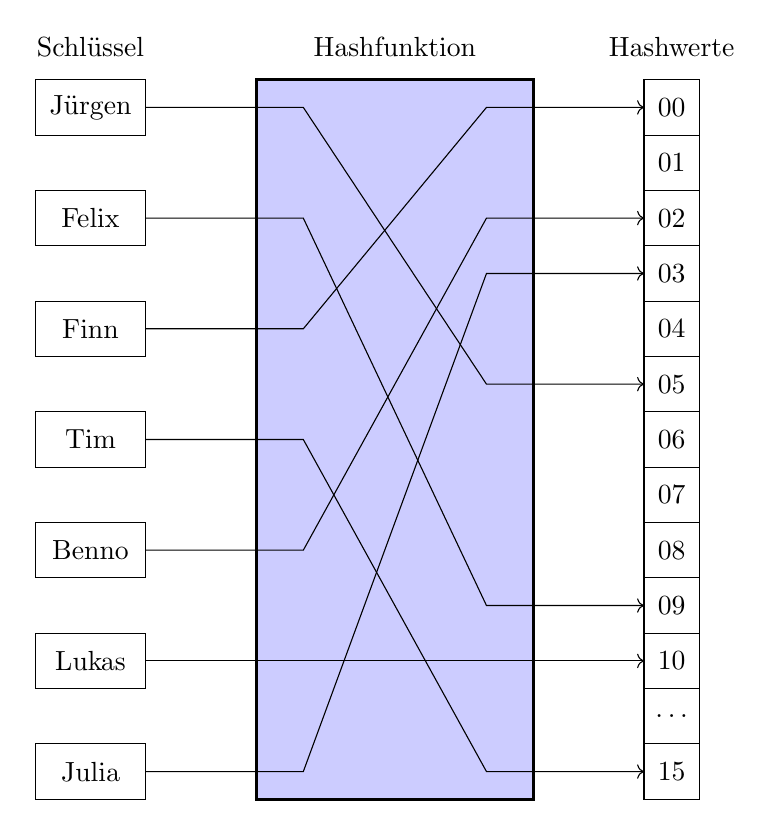
\begin{tikzpicture}[
            %  -{Stealth[length = 2.5pt]},
            start chain = going {right=of \tikzchainprevious.north east},
            KeyBlock/.style={minimum width=4em, minimum height=2em, outer sep=0pt, on chain},
            HashBlock/.style={minimum width=2em, minimum height=2em, outer sep=0pt, on chain},
            FunctionBlock/.style={minimum width=10em, minimum height=26em, outer sep=0pt, on chain, very thick,fill=blue!20},
            every node/.style={draw, label distance=0.5em},
            every on chain/.style={anchor=north west},
            node distance=4em
            ]
            {
            \node [KeyBlock, label=above:Schlüssel] (k0) {Jürgen};
            \node [FunctionBlock, label=above:Hashfunktion] (fun) {};
            \node [HashBlock, label=above:Hashwerte] (h00) {00};

            { [continue chain = going {below=of \tikzchainprevious.south west}, node distance=2em]
            \chainin (k0);
            \node [KeyBlock] (k1) {Felix};
            \node [KeyBlock] (k2) {Finn};
            \node [KeyBlock] (k3) {Tim};
            \node [KeyBlock] (k4) {Benno};
            \node [KeyBlock] (k5) {Lukas};
            \node [KeyBlock] (k6) {Julia};
            }

            { [continue chain = going {below=of \tikzchainprevious.south west}, node distance=0pt]
            \chainin (h00);
            \node [HashBlock] (h01) {01};
            \node [HashBlock] (h02) {02};
            \node [HashBlock] (h03) {03};
            \node [HashBlock] (h04) {04};
            \node [HashBlock] (h05) {05};
            \node [HashBlock] (h06) {06};
            \node [HashBlock] (h07) {07};
            \node [HashBlock] (h08) {08};
            \node [HashBlock] (h09) {09};
            \node [HashBlock] (h10) {10};
            \node [HashBlock] (hdots) {$\ldots$};
            \node [HashBlock] (h15) {15};
            }

            \draw[->] (k0.east) -- ++(2, 0) -- ($(h05.west)-(2,0)$) -- (h05.west);
            \draw[->] (k1.east) -- ++(2, 0) -- ($(h09.west)-(2,0)$) -- (h09.west);
            \draw[->] (k2.east) -- ++(2, 0) -- ($(h00.west)-(2,0)$) -- (h00.west);
            \draw[->] (k3.east) -- ++(2, 0) -- ($(h15.west)-(2,0)$) -- (h15.west);
            \draw[->] (k4.east) -- ++(2, 0) -- ($(h02.west)-(2,0)$) -- (h02.west);
            \draw[->] (k5.east) -- ++(2, 0) -- ($(h10.west)-(2,0)$) -- (h10.west);
            \draw[->] (k6.east) -- ++(2, 0) -- ($(h03.west)-(2,0)$) -- (h03.west);
            }
        \end{tikzpicture}
    \end{center}
\end{defi}

\begin{example}{Divisions-Hash}
    Die \emph{Divisionsrest-Methode (Divisions-Hash)} um Integer zu hashen wird definiert durch:
    $$
        h(x) = x \operatorname{mod} N
    $$

    Sie wird bevorzugt, wenn die Schlüsselverteilung nicht bekannt ist.
    Etwaige Regelmäßigkeiten in der Schlüsselverteilung sollte sich nicht in der Adressverteilung auswirken. Daher sollte $N$ eine Primzahl sein.
\end{example}

\begin{example}{Hashfunktionen für verschiedene Datentypen}
    \begin{itemize}
        \item Alle Datenypen: Verwenden der Speicheradresse
        \item Strings: ASCII/Unicode-Werte addieren (evtl. von einigen Buchstaben, evtl. gewichtet)
    \end{itemize}
\end{example}

\begin{defi}{Kollision}
    Sei $S$ eine Schlüsselmenge und $h$ eine Hashfunktion.
    Ist
    $$
        s_1, s_2 \in S, \ s_1 \neq s_2 : h(s_1) = h(s_2)
    $$
    so spricht man von einer \emph{Kollision}.

    Die Wahrscheinlichkeit von Kollisionen ist abhängig von der gewählten Hashfunktion.
    Hashfunktionen sollten also möglichst gut \emph{streuen}, aber dennoch effizient berechenbar sein.

    \begin{center}
        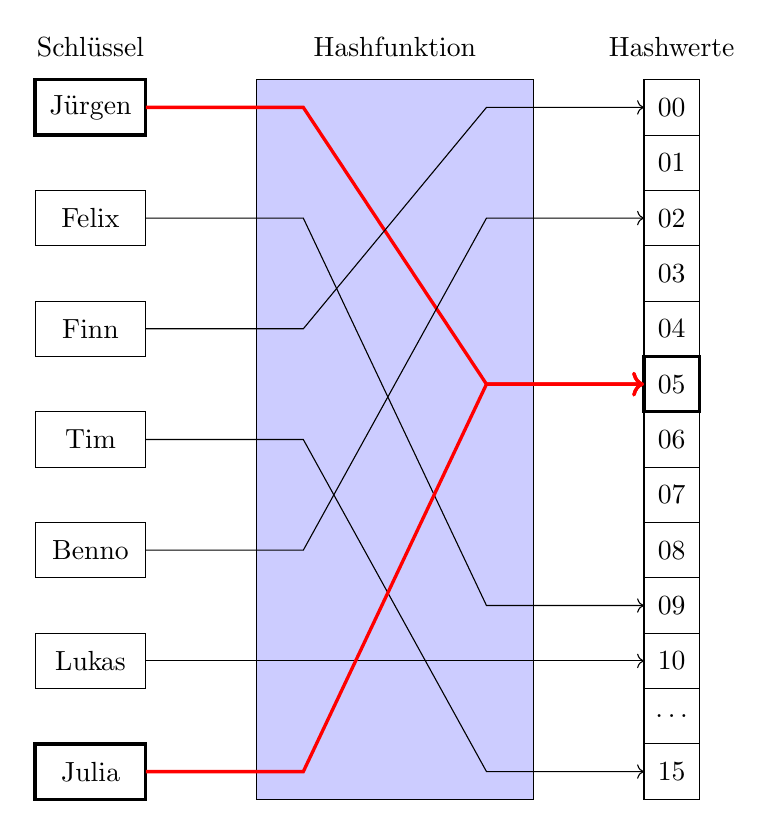
\begin{tikzpicture}[
            %  -{Stealth[length = 2.5pt]},
            start chain = going {right=of \tikzchainprevious.north east},
            KeyBlock/.style={minimum width=4em, minimum height=2em, outer sep=0pt, on chain},
            HashBlock/.style={minimum width=2em, minimum height=2em, outer sep=0pt, on chain},
            FunctionBlock/.style={minimum width=10em, minimum height=26em, outer sep=0pt, on chain,fill=blue!20},
            every node/.style={draw, label distance=0.5em},
            every on chain/.style={anchor=north west},
            node distance=4em
            ]
            {
            \node [KeyBlock, label=above:Schlüssel, very thick] (k0) {Jürgen};
            \node [FunctionBlock, label=above:Hashfunktion] (fun) {};
            \node [HashBlock, label=above:Hashwerte] (h00) {00};

            { [continue chain = going {below=of \tikzchainprevious.south west}, node distance=2em]
            \chainin (k0);
            \node [KeyBlock] (k1) {Felix};
            \node [KeyBlock] (k2) {Finn};
            \node [KeyBlock] (k3) {Tim};
            \node [KeyBlock] (k4) {Benno};
            \node [KeyBlock] (k5) {Lukas};
            \node [KeyBlock, very thick] (k6) {Julia};
            }

            { [continue chain = going {below=of \tikzchainprevious.south west}, node distance=0pt]
            \chainin (h00);
            \node [HashBlock] (h01) {01};
            \node [HashBlock] (h02) {02};
            \node [HashBlock] (h03) {03};
            \node [HashBlock] (h04) {04};
            \node [HashBlock, very thick] (h05) {05};
            \node [HashBlock] (h06) {06};
            \node [HashBlock] (h07) {07};
            \node [HashBlock] (h08) {08};
            \node [HashBlock] (h09) {09};
            \node [HashBlock] (h10) {10};
            \node [HashBlock] (hdots) {$\ldots$};
            \node [HashBlock] (h15) {15};
            }

            \draw[->, very thick, color=red] (k0.east) -- ++(2, 0) -- ($(h05.west)-(2,0)$) -- (h05.west);
            \draw[->] (k1.east) -- ++(2, 0) -- ($(h09.west)-(2,0)$) -- (h09.west);
            \draw[->] (k2.east) -- ++(2, 0) -- ($(h00.west)-(2,0)$) -- (h00.west);
            \draw[->] (k3.east) -- ++(2, 0) -- ($(h15.west)-(2,0)$) -- (h15.west);
            \draw[->] (k4.east) -- ++(2, 0) -- ($(h02.west)-(2,0)$) -- (h02.west);
            \draw[->] (k5.east) -- ++(2, 0) -- ($(h10.west)-(2,0)$) -- (h10.west);
            \draw[->, very thick, color=red] (k6.east) -- ++(2, 0) -- ($(h05.west)-(2,0)$) -- (h05.west);
            }
        \end{tikzpicture}
    \end{center}

\end{defi}

\begin{defi}{Kollisionsbehandlung}
    Um Kollisionen zu handhaben, existieren verschiedene Strategien:
    \begin{itemize}
        \item \emph{Hashing mit Verkettung}
              \begin{itemize}
                  \item Hashtabelle besteht aus $N$ linearen Listen
                  \item $h(s)$ gibt dann an, in welche Teilliste der Datensatz gehört
                  \item Daten werden innerhalb der Teillisten sequentiell gespeichert
              \end{itemize}
        \item \emph{Hashing mit offener Adressierung}
              \begin{itemize}
                  \item Suchen einer alternativen Position innerhalb des Feldes
                        \begin{enumerate}
                            \item Lineares Sondieren (Verschiebung um konstantes Intervall)
                            \item Doppeltes Hashing (Nutzen einer weiteren Hashfunktion)
                            \item Quadratisches Sondieren (Intervall wird quadriert)
                        \end{enumerate}
              \end{itemize}
    \end{itemize}
\end{defi}

\begin{defi}{Schrittzahl}
    Die \emph{Schrittzahl} $S(s)$, die nötig ist, um den Datensatz mit Schlüssel $s$ zu speichern bzw. wiederzufinden, setzt sich z.B. beim Hashing mit Verkettung zusammen aus:
    \begin{itemize}
        \item der Berechnung der Hash-Funktion und
        \item dem Aufwand für die Suche bzw. Speicherung innerhalb der Teilliste.
    \end{itemize}
\end{defi}

\begin{defi}{Füllgrad}
    Der \emph{Füllgrad} einer Hashtabelle ist der Quotient
    $$
        \alpha = \frac{n}{N}
    $$
    mit
    \begin{itemize}
        \item $N$ als Größe der Hashtabelle
        \item $n$ als Anzahl der gespeicherten Datensätze
    \end{itemize}
\end{defi}

\begin{example}{Schrittzahl beim Suchen in Teillisten}
    Bei idealer Speicherung entfallen $\alpha$ Elemente auf jede Teilliste.
    Dabei gilt:
    \begin{itemize}
        \item erfolgreiche Suche: $c_1 + c_2 \cdot \frac{\alpha}{2}$
        \item erfolglose Suche: $c_1 + c_2 \cdot \alpha$
    \end{itemize}
    Damit ist der Suchaufwand in $\bigo(\alpha) = \bigo(\frac{n}{N})$.

    Wird der Füllgrad $\alpha$ zu groß, sollte die Hashtabelle vergrößert werden.
\end{example}

\begin{defi}{Dynamisches Hashing}
    Um viele Kollisionen zu vermeiden, muss die Hashtabelle ab einem gewissen Füllgrad vergrößert werden.\footnote{nach Sedgewick sollte stets $\alpha < 0.5$ gelten}

    Als Folge muss die gesamte Hashtabelle aber auch neu aufgebaut werden.
\end{defi}

\begin{defi}{Offene Adressierung (Sondieren)}
    Beim Speichern wird bei \emph{Hashing mit offener Adressieren (Sondierung)} so lang ein neuer Hashindex berechnet, bis dort ein freier Speicherplatz vorhanden ist.

    Das Suchen funktioniert analog, allerdings ist das Löschen sehr aufwändig.

    \begin{itemize}
        \item Lineares Sondieren
              \begin{itemize}
                  \item Wird die Ersatzadresse bei jeder Kollision durch Erhöhen der alten Adresse um 1 berechnet, so spricht man von \emph{linearem Sondieren (linear probing)}.
                  \item Die $i$-te Ersatzadresse für einen Schlüssel $s$ mit Hashindex $h(s)$ wird also wie folgt berechnet:
                        $$
                            h_i(s) = (h(s) + i) \operatorname{mod} N
                        $$
              \end{itemize}
        \item Doppeltes Hashing
              \begin{itemize}
                  \item Schlüssel wird nicht um $1$ erhöht, sondern der Inkrement wird mit einer zweiten Hashfunktion berechnet.
                  \item Beseitigt praktisch die Probleme der primären und sekundären Häufung.
                  \item Nicht alle Felder werden durchprobiert. Im ungünstigsten Fall kann eine neues Element nicht eingefügt werden, auch wenn noch Felder frei sind.
              \end{itemize}
    \end{itemize}
\end{defi}

\begin{defi}{Primäre und sekundäre Häufung}
    Bei der \emph{primären Häufung (primary clustering)} ist die Wahrscheinlichkeit, dass Plätze in einem dichtbelegten Bereich eher besetzt werden, deutlich höher.
    Es kommt also zu Kettenbildung.

    Besonders häufig tritt primäre Häufung z.B. beim linearen Sondieren auf.

    \begin{center}
        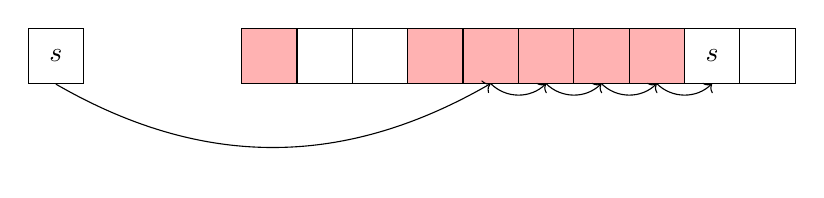
\begin{tikzpicture}
            [
                %  -{Stealth[length = 2.5pt]},
                start chain,
                node distance = 0pt,
                StackBlock/.style={draw, minimum width=2em, minimum height=2em, outer sep=0pt, on chain},
            ]

            \node [draw, minimum width=2em, minimum height=2em] (val) {$s$};

            { start chain = going right
            \node [StackBlock,right=2cm of val,fill=red!30] (0) {};
            \node [StackBlock] (1) {};
            \node [StackBlock] (2) {};
            \node [StackBlock,fill=red!30] (3) {};
            \node [StackBlock,fill=red!30] (4) {};
            \node [StackBlock,fill=red!30] (5) {};
            \node [StackBlock,fill=red!30] (6) {};
            \node [StackBlock,fill=red!30] (7) {};
            \node [StackBlock] (8) {$s$};
            \node [StackBlock] (9) {};

            \draw[->] (val.south) [out=-30, in=-150] to (4.south);
            \draw[->] (4.south) [out=-45, in=-135] to (5.south);
            \draw[->] (5.south) [out=-45, in=-135] to (6.south);
            \draw[->] (6.south) [out=-45, in=-135] to (7.south);
            \draw[->] (7.south) [out=-45, in=-135] to (8.south);
            }
        \end{tikzpicture}
    \end{center}


    Die \emph{sekundäre Häufung (secondary clustering)} hängt von der Hashfunktion ab.
    Dabei durchlaufen zwei Schlüssel $h(s)$ und $h(s')$ stets dieselbe Sondierungsfolge.
    Sie behindern sich also auf den Ausweichplätzen.

    Besonders häufig tritt sekundäre Häufung z.B. beim quadratischen Sondieren auf.


    \begin{center}
        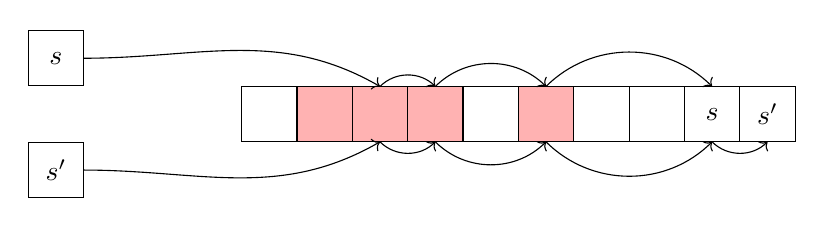
\begin{tikzpicture}
            [
                %  -{Stealth[length = 2.5pt]},
                start chain,
                node distance = 0pt,
                StackBlock/.style={draw, minimum width=2em, minimum height=2em, outer sep=0pt, on chain},
            ]

            \node [minimum width=2em, minimum height=2em] (val) {};

            { start chain = going right
            \node [StackBlock,right=2cm of val] (0) {};
            \node [StackBlock,fill=red!30] (1) {};
            \node [StackBlock,fill=red!30] (2) {};
            \node [StackBlock,fill=red!30] (3) {};
            \node [StackBlock] (4) {};
            \node [StackBlock,fill=red!30] (5) {};
            \node [StackBlock] (6) {};
            \node [StackBlock] (7) {};
            \node [StackBlock] (8) {$s$};
            \node [StackBlock] (9) {$s'$};

            { [continue chain = going above]
            \chainin (val);
            \node [StackBlock] (val1) {$s$};
            }

            { [continue chain = going below]
            \chainin (val);
            \node [StackBlock] (val2) {$s'$};
            }

            \draw[->] (val1.east) [out=0, in=150] to (2.north);
            \draw[->] (2.north) [out=45, in=135] to (3.north);
            \draw[->] (3.north) [out=45, in=135] to (5.north);
            \draw[->] (5.north) [out=45, in=135] to (8.north);

            \draw[->] (val2.east) [out=0, in=-150] to (2.south);
            \draw[->] (2.south) [out=-45, in=-135] to (3.south);
            \draw[->] (3.south) [out=-45, in=-135] to (5.south);
            \draw[->] (5.south) [out=-45, in=-135] to (8.south);
            \draw[->] (8.south) [out=-45, in=-135] to (9.south);
            }
        \end{tikzpicture}
    \end{center}
\end{defi}


\section{Bäume}

\begin{defi}{Baum}
    Ein \emph{Baum} ist eine hierarchische (rekursive) Datenstruktur.
    Es gilt:
    \begin{itemize}
        \item alle Wege gehen von einer \emph{Wurzel} aus
        \item $A$ heißt \emph{Vorgänger} von $B$ bzw. $B$ \emph{Nachfolger} von $A$, wenn $A$ auf einem Weg von der Wurzel zu $B$ liegt
        \item $A$ heißt \emph{Elterknoten} von $B$, bzw. $B$ heißt \emph{Kind} von $A$, wenn $(A, B) \in E$
        \item Knoten ohne Kinder heißen \emph{Blätter}
        \item Knoten mit Kindern heißen \emph{innere Knoten}
        \item ein Knoten $S$ mit allen Nachfolgern wird \emph{Teilbaum} eines Baumes $T$ genannt, falls $S$ nicht Wurzel von $T$ ist
        \item der \emph{Verzweigungsgrad} eines Knotens ist die Anzahl seiner Kinder
    \end{itemize}

    \vspace{1em}

    \begin{center}
        \begin{forest}
            for tree={s sep=5mm, fit=band}
            [Wurzel, name=root
            [Blatt, name=blatt1]
            [Innerer Knoten, name=inner1 [Blatt, name=blatt2]
            [Innerer Knoten, name=inner2
            [Blatt, name=blatt3]
            [Innerer Knoten, name=inner3 [Blatt, name=blatt4]
            [Blatt, name=blatt5]]]]]
            \node [draw, label=left:Level 0, dashed, fit={(root) (blatt1.west |- root.center) (inner3.east |- root.center)}] {};
            \node [draw, label=left:Level 1, dashed, fit={(blatt1) (inner3.east |- blatt1.center)}] {};
            \node [draw, label=left:Level 2, dashed, fit={(blatt2) (blatt1.west |- blatt2.center) (inner3.east |- blatt2.center)}] {};
            \node [draw, label=left:Level 3, dashed, fit={(blatt3) (blatt1.west |- blatt3.center) (inner3)}] {};
            \node [draw, label=left:Level 4, dashed, fit={(blatt4) (blatt1.west |- blatt5.center) (blatt5) (inner3.east |- blatt5.center)}] {};
            \node [draw, red, fit={(inner2) (inner3) (blatt5) (blatt3)},label=right:{\color{red}Teilbaum}] {};
        \end{forest}
    \end{center}
\end{defi}

% Binärbäume

\begin{defi}{Binärbaum}
    Die Knoten eines \emph{Binärbaums (binary tree)} haben höchstens den Verzweigungsgrad $2$.

    Bei einem \emph{geordneten Binärbaum} ist die Reihenfolge der Kinder durch die Indizes eindeutig festgelegt:
    \begin{itemize}
        \item $T_l$: linkes Kind, linker Teilbaum
        \item $T_r$: rechtes Kind, rechter Teilbaum
    \end{itemize}

    Ein Binärbaum heißt \emph{minimal} (bezogen auf die Höhe), wenn kein Binärbaum mit gleicher Knotenzahl aber kleinerer Höhe existiert.

    Ein \emph{links-vollständiger Binärbaum} ist ein minimaler Binärbaum, in dem die Knoten auf dem untersten Level so weit wie möglich links stehen.

    Alle Blätter eines \emph{vollständigen Binärbaums} haben den gleichen Level und dieser ist vollbesetzt.

    Ein vollständiger Binärbaum der Höhe $H$ hat
    $$
        n = 1 + 2 + 4 + \ldots + 2^H = \frac{2^{H+1}-1}{2-1} = 2^{H+1}-1 \ \text{Knoten}
    $$
\end{defi}

\begin{halfboxl}
    \begin{example}{Linksvollständiger Binärbaum}
        \centering
        \begin{forest}
            for tree={circle, draw,
            minimum size=1.75em, % <-- added
            inner sep=1pt}
            [
            [
                    [
                            []
                                []
                        ]
                        [
                            []
                                []
                        ]
                ]
                [
                    []
                        []
                ]
            ]
        \end{forest}
    \end{example}
\end{halfboxl}
\begin{halfboxr}
    \begin{example}{Vollständiger Binärbaum}
        \centering
        \begin{forest}
            for tree={circle, draw,
            minimum size=1.75em, % <-- added
            inner sep=1pt}
            [
            [
                    [
                            []
                                []
                        ]
                        [
                            []
                                []
                        ]
                ]
                [
                    [
                            []
                                []
                        ]
                        [
                            []
                                []
                        ]
                ]
            ]
        \end{forest}
    \end{example}
\end{halfboxr}

\subsection{Binäre Suchbäume}
% Binäre Suchbäume

\begin{defi}{Binärer Suchbaum}
    Ein \emph{binärer Suchbaum} ist ein Binärbaum, bei dem für jeden Knoten des Baumes gilt:

    Alle Schlüssel im linken Teilbaum sind kleiner, alle im rechten Teilbaum sind größer oder gleich dem Schlüssel in diesem Knoten.
\end{defi}

\begin{algo}{Suchen im binären Suchbaum}
    Suchen ist ohne Probleme durch einfaches Vergleichen ($<$ bzw. $\geq$) möglich.

    Suchen der $50$ in \textcolor{red}{rot} bzw. (erfolgloses) Suchen der $80$ in \textcolor{blue}{blau}.

    \vspace{1em}

    \centering
    \forestset{%
        empty node/.style={dashed}
    }
    \begin{forest}
        for tree={circle, draw,
        minimum size=2em, % <-- added
        inner sep=1pt}
        [60
        [
        20,edge={->,dashed,red,thick}
        [10 [,empty node][,empty node]]
        [30,edge={->,dashed,red,thick}
        [,empty node]
        [50,edge={->,dashed,red,thick}, draw=red [,empty node][,empty node]]
        ]
        ]
        [
        70,edge={->,dashed,blue,thick}
            [,empty node]
            [110,edge={->,dashed,blue,thick}
                    [90,edge={->,dashed,blue,thick}
                            [,empty node,edge={->,dashed,blue,thick},draw=blue][,empty node]
                    ]
                    [,empty node]
            ]
        ]
        ]
    \end{forest}
\end{algo}

\begin{algo}{Einfügen im binären Suchbaum}
    Ein Knoten kann ohne Probleme hinzugefügt werden, indem man solange sucht, bis man auf einen leeren Kindknoten trifft und dort einfügt.

    Einfügen der $40$ in \textcolor{red}{rot}.

    \vspace{1em}

    \centering
    \begin{forest}
        for tree={circle, draw,
        minimum size=2em, % <-- added
        inner sep=1pt}
        [60
            [
                20,edge={->,dashed,red,thick}
                    [10 [,empty node][,empty node]]
                    [30,edge={->,dashed,red,thick}
                            [,empty node]
                            [50,edge={->,dashed,red,thick} [
                                        40,edge={->,dashed,red,thick},draw=red
                                    ][,empty node]]
                    ]
            ]
            [
                70
                    [,empty node]
                    [110
                            [90
                                    [,empty node][,empty node]
                            ]
                            [,empty node]
                    ]
            ]
        ]
    \end{forest}
\end{algo}

\begin{algo}{Löschen im binären Suchbaum (Blatt)}
    Ein Blatt kann problemlos gelöscht werden.

    Löschen der $50$ in \textcolor{red}{rot}.

    \vspace{1em}

    \centering
    \begin{forest}
        baseline,anchor=north,
        for tree={circle, draw,
        minimum size=2em, % <-- added
        inner sep=1pt}
        [20,edge={->,dashed,red,thick}
        [10
            [,empty node]
            [,empty node]
        ]
        [30,edge={->,dashed,red,thick}
        [,empty node]
        [50,edge={->,dashed,red,thick}, draw=red
        [,empty node]
        [,empty node]
        ]
        ]
        ]
    \end{forest}
    \hspace{5em}
    \begin{forest}
        baseline,anchor=north,
        for tree={circle, draw,
                minimum size=2em, % <-- added
                inner sep=1pt}
            [20
                    [10
                            [,empty node]
                            [,empty node]
                    ]
                    [30
                            [,empty node]
                            [,empty node,draw=red]
                    ]
            ]
    \end{forest}
\end{algo}

\begin{algo}{Löschen im binären Suchbaum (Innerer Knoten mit einem Kind)}
    Soll ein innerer Knoten mit einem Kind gelöscht werden, rückt das Kind an die Stelle des Elterknotens.

    Löschen der $30$ in \textcolor{red}{rot}.

    \vspace{1em}

    \centering
    \begin{forest}
        baseline,anchor=north,
        for tree={circle, draw,
        minimum size=2em, % <-- added
        inner sep=1pt}
        [20,edge={->,dashed,red,thick}
        [10
            [,empty node]
            [,empty node]
        ]
        [30,edge={->,dashed,red,thick}, draw=red
        [,empty node]
        [50,draw=blue
        [,empty node]
        [,empty node]
        ]
        {\draw[->,blue] () to[bend right=45] node[midway,above right,font=\small]{Vorrücken} (!u.east);}
        ]
        ]
    \end{forest}
    \hspace{5em}
    \begin{forest}
        baseline,anchor=north,
        for tree={circle, draw,
        minimum size=2em, % <-- added
        inner sep=1pt}
        [20
        [10
            [,empty node]
            [,empty node]
        ]
        [50,draw=blue
        [,empty node]
        [,empty node]
        ]
        ]
    \end{forest}
\end{algo}

\begin{algo}{Löschen im binären Suchbaum (Innerer Knoten mit zwei Kindern)}
    Soll ein innerer Knoten mit zwei Kindern gelöscht werden, nimmt der nächstgrößere Knoten seinen Platz ein.

    Dieser wird wie folgt ermittelt (in \textcolor{purple}{lila}):
    \begin{enumerate}
        \item Gehe einen Schritt nach rechts.
        \item Gehe solange nach links, bis es kein linkes Kind mehr gibt.
    \end{enumerate}

    Löschen der $20$ in \textcolor{red}{rot}.

    \vspace{1em}

    \centering
    \begin{forest}
        baseline,anchor=north,
        for tree={circle, draw,
        minimum size=2em, % <-- added
        inner sep=1pt}
        [20,draw=red
        [10
            [,empty node]
            [,empty node]
        ]
        [30,edge={->,dashed,purple,thick},draw=purple
        [,empty node,edge={->,dashed,purple,thick}]
        [50
            [,empty node]
            [,empty node]
        ]
        ]{\draw[->,blue] () to[bend right=45] node[midway,above right,font=\small]{Platz einnehmen} (!u.east);}
        ]
    \end{forest}
    %\hspace{1em}
    \begin{forest}
        baseline,anchor=north,
        for tree={circle, draw,
        minimum size=2em, % <-- added
        inner sep=1pt}
        [30,draw=purple
        [10
            [,empty node]
            [,empty node]
        ]
        [,empty node
        %[,empty node]
        [50,draw=blue
        [,empty node]
        [,empty node]
        ]
        {\draw[->,blue] () to[bend right=45] node[midway,above right,font=\small]{Vorrücken} (!u.east);}
        ]
        ]
    \end{forest}
    %\hspace{1em}
    \begin{forest}
        baseline,anchor=north,
        for tree={circle, draw,
        minimum size=2em, % <-- added
        inner sep=1pt}
        [30,draw=purple
        [10
            [,empty node]
            [,empty node]
        ]
        [50,draw=blue
        [,empty node]
        [,empty node]
        ]
        ]
    \end{forest}
\end{algo}

\begin{bonus}{Komplexität beim Suchen, Löschen und Einfügen in Binärbäumen}
    Die Komplexität der Funktionen Suchen, Löschen und Einfügen werden durch die Komplexität des Suchens eines Elements bestimmt.

    Im schlechtesten Fall ist die Anzahl der zu durchsuchenden Elemente gleich der Höhe des Baumes $+1$.
    Dabei hängt die Höhe stark von der Reihenfolge der Einfügeoperationen ab.

    \vspace{1em}

    \centering
    \begin{forest}
        baseline,anchor=north,
        for tree={circle, draw,
                minimum size=2em, % <-- added
                inner sep=1pt}
            [10
                    [,empty node]
                    [
                        20
                            [,empty node]
                            [
                                30
                                    [,empty node]
                                    [
                                        40
                                            [,empty node]
                                            [
                                                50
                                                    [,empty node]
                                                    [
                                                        60
                                                            [,empty node]
                                                            [,empty node]
                                                    ]
                                            ]
                                    ]
                            ]
                    ]
            ]
    \end{forest}
    \hspace{5em}
    \begin{forest}
        baseline,anchor=north,
        for tree={circle, draw,
                minimum size=2em, % <-- added
                inner sep=1pt}
            [
                40
                    [
                        20
                            [
                                10
                                    [,empty node]
                                    [,empty node]
                            ]
                            [
                                30
                                    [,empty node]
                                    [,empty node]
                            ]
                    ]
                    [
                        50
                            [,empty node]
                            [
                                60
                                    [,empty node]
                                    [,empty node]
                            ]
                    ]
            ]
    \end{forest}
\end{bonus}

% Balancierte Bäume

\begin{defi}{Balanciertheit}

    Ein Binärbaum mit $n$ Knoten hat im besten Fall (\emph{optimal balanciert}) die Höhe
    $$
        H = \lceil \log_2(n+1) \rceil - 1 = \lfloor \log_2(n) \rfloor
    $$
    Dabei ist Suchen in $\bigo(\log n)$.

    Ein Binärbaum mit $n$ Knoten hat im schlechtesten Fall (\emph{entartet/degeneriert}) die Höhe
    $$
        H = n-1
    $$
    Dabei ist Suchen in $\bigo(n)$.
\end{defi}

\begin{defi}{Balance-Kriterien}
    \begin{enumerate}
        \item Abgeschwächtes Kriterium für ausgeglichene Höhe
              \begin{itemize}
                  \item lokale Umordnungsoperationen reichen aus
                  \item z.B. \emph{AVL-Bäume} und Rot-Schwarz-Bäume
              \end{itemize}
        \item Jeder neue Knoten wandert an die Wurzel des Baumes
              \begin{itemize}
                  \item Vorteil: Zuletzt eingefügte Elemente lassen sich schneller finden
                  \item durch spezielles Einfügeverfahren wird Baum zusätzlich (teilweise) ausgeglichen
                  \item z.B. Splay-Bäume
              \end{itemize}
        \item Unausgeglichener Verzweigungsgrad ermöglicht ausgeglichene Höhe
              \begin{itemize}
                  \item z.B. \emph{B-Bäume}
              \end{itemize}
    \end{enumerate}
\end{defi}

\subsection{AVL-Bäume}

% AVL-Bäume

\begin{defi}{AVL-Baum}
    Bei einem \emph{AVL-Baum} unterscheiden sich die Höhen zweier Teilbäume des gleichen Knotens maximal um $1$.

    Der sogenannte \emph{Balance-Index} (oder Balance-Faktor) $\BF$ eines Knotens $T$ ist die Differenz
    $$
        \BF(T) := H(T_r) - H(T_l)
    $$
    Dabei gilt:
    \begin{itemize}
        \item Jeder Knoten hat einen Balance-Index.
        \item Er darf nur die Werte $-1$, $0$ oder $1$ annehmen.
    \end{itemize}

    %\vspace{2em}

    \centering
    \begin{forest}
        baseline,anchor=north,
        for tree={circle, draw,
        minimum size=2em, % <-- added
        inner sep=1pt}
        [
        J, label=right:{\small\textcolor{blue}{+1}}
        [
        F, label=right:{\small\textcolor{blue}{-1}}
        [
        D, label=right:{\small\textcolor{blue}{-1}}
        [
        C, label=left:{\small\textcolor{blue}{0}}
        [,empty node]
        [,empty node]
        ]
        [,empty node]
        ]
        [
        G, label=right:{\small\textcolor{blue}{0}}
        [,empty node]
        [,empty node]
        ]
        ]
        [
        P, label=right:{\small\textcolor{blue}{+1}}
        [
        L, label=right:{\small\textcolor{blue}{+1}}
        [,empty node]
        [
        N, label=right:{\small\textcolor{blue}{0}}
        [,empty node]
        [,empty node]
        ]
        ]
        [
        V, label=right:{\small\textcolor{blue}{-1}}
        [
        S, label=right:{\small\textcolor{blue}{0}}
        [
        Q, label=right:{\small\textcolor{blue}{0}}
        [,empty node]
        [,empty node]
        ]
        [
        U, label=left:{\small\textcolor{blue}{0}}
        [,empty node]
        [,empty node]
        ]
        ]
        [
        X, label=right:{\small\textcolor{blue}{0}}
        [,empty node]
        [,empty node]
        ]
        ]
        ]
        ]
    \end{forest}
\end{defi}

\begin{algo}{Einfügen in einem AVL-Baum}
    Beim Einfügen in einen AVL-Baum wird zu Beginn analog zu einem regulären Binärbaum eingefügt.

    Anschließend wird sich der unmittelbare Elterknoten $E$ angeschaut und es gibt für den dortigen Balance-Index $\BF(E)$ drei Fälle:
    \begin{enumerate}
        \item $\BF(E)$ wird $0$:
              \begin{itemize}[-]
                  \item $\BF(E)$ war vorher $-1$
                  \item man kommt von einem Kindbaum, der vorher niedriger war
                  \item Höhe des Knotens ändert sich nicht
                  \item oberhalb bleiben alle Balance-Indizes gleich
                  \item $\implies$ AVL-Kriterium ist für den ganzen Baum erfüllt
              \end{itemize}
        \item $\BF(E)$ wird $\pm 1$:
              \begin{itemize}[-]
                  \item $\BF(E)$ war vorher $0$
                  \item Höhe des Teilbaums erhöht sich um $1$
                  \item $\implies$ Überprüfung der Balance-Indizes muss beim Elternknoten von $E$ fortgesetzt werden
              \end{itemize}
        \item $\BF(E)$ wird $\pm 2$:
              \begin{itemize}[-]
                  \item $\BF(E)$ war vorher $\pm 1$
                  \item $\implies$ Teilbaum muss \emph{rebalanciert} werden
              \end{itemize}
    \end{enumerate}
\end{algo}

\begin{algo}{Löschen in einem AVL-Baum}
    Beim Löschen in einen AVL-Baum wird zu Beginn analog zu einem regulären Binärbaum gelöscht.

    Anschließend wird sich der unmittelbare Elterknoten $E$ angeschaut und es gibt für den dortigen Balance-Index $\BF(E)$ drei Fälle:
    \begin{enumerate}
        \item $\BF(E)$ wird $\pm 1$:
              \begin{itemize}[-]
                  \item $\BF(E)$ war vorher $0$
                  \item Höhe des Knotens ändert sich nicht
                  \item oberhalb bleiben alle Balance-Indizes gleich
                  \item $\implies$ AVL-Kriterium ist für den ganzen Baum erfüllt
              \end{itemize}
        \item $\BF(E)$ wird $0$:
              \begin{itemize}[-]
                  \item $\BF(E)$ war vorher $0$
                  \item Höhe des Teilbaums verringert sich um $1$
                  \item $\implies$ Überprüfung der Balance-Indizes muss beim Elternknoten von $E$ fortgesetzt werden
              \end{itemize}
        \item $\BF(E)$ wird $\pm 2$:
              \begin{itemize}[-]
                  \item $\BF(E)$ war vorher $\pm 1$
                  \item $\implies$ Teilbaum muss \emph{rebalanciert} werden
              \end{itemize}
    \end{enumerate}
\end{algo}

\begin{algo}{Rebalancierung}
    Wenn bei einer Opeation ein Höhenunterschied von mehr als $1$ zwischen zwei Geschwister-Teilbäumen entsteht, ist beim Elterknoten das AVL-Kriterium verletzt.
    Eine entsprechende Korrektur heißt \emph{Rebalancierung}.
    Als Werkzeuge eignen sich hierfür die sogenannten \emph{Rotationen}.
\end{algo}

\begin{algo}{Einfachrotation}
    Wird ein AVL-Baum unbalanciert, wenn ein Knoten in den \emph{rechten Teilbaum des rechten Teilbaums} eingefügt wird (Rechts-Rechts-Situation), dann wird das durch eine \emph{Einfachrotation nach links} gelöst.

    Zuletzt wurde $9$ eingefügt. Linksrotation in \textcolor{purple}{lila}.

    \vspace{1em}

    \begin{center}
        \begin{forest}
            baseline,anchor=north,
            for tree={circle, draw,
            minimum size=2em, % <-- added
            inner sep=1pt}
            [3%, label=right:{\small\textcolor{red}{+2}}
            [1%, label=below right:{\small\textcolor{blue}{0}}
                [,empty node]
                [,empty node]
            ]
            [7, label=above:{\small\textcolor{red}{+2}}, draw=teal, name=7
            [,empty node]
            [8, label=right:{\small\textcolor{blue}{+1}}, draw=purple, edge={teal,thick}
            [,empty node, name=8c]
            [9, label=right:{\small\textcolor{blue}{0}}, edge={purple,thick},draw=purple
            ]
            ]
            {\draw[->,purple] () to[bend right=45] node[midway,above right,font=\small]{Linksrotation} (!u.east);}
            ]
            ]
            \draw[->,teal] (7) to[bend right=45] (8c);
        \end{forest}
        \hspace{5em}
        \begin{forest}
            baseline,anchor=north,
            for tree={circle, draw,
            minimum size=2em, % <-- added
            inner sep=1pt}
            [3, label=right:{\small\textcolor{blue}{+1}}
            [1, label=right:{\small\textcolor{blue}{0}}
            [,empty node]
            [,empty node]
            ]
            [8, label=right:{\small\textcolor{blue}{0}}, draw=purple
            [7, label=right:{\small\textcolor{blue}{0}}, draw=teal, edge={teal,thick}
                [,empty node]
                [,empty node]
            ]
            [9, label=right:{\small\textcolor{blue}{0}}, edge={purple,thick},draw=purple
            [,empty node]
            [,empty node]
            ]
            ]
            ]
        \end{forest}
    \end{center}

    \vspace{1em}

    Wird ein AVL-Baum unbalanciert, wenn ein Knoten in den \emph{linken Teilbaum des linken Teilbaums} eingefügt wird (Links-Links-Situation), dann wird das durch eine \emph{Einfachrotation nach rechts} gelöst.

    Zuletzt wurde $1$ eingefügt. Rechtsrotation in \textcolor{purple}{lila}.

    \vspace{1em}

    \begin{center}
        \begin{forest}
            baseline,anchor=north,
            for tree={circle, draw,
            minimum size=2em, % <-- added
            inner sep=1pt}
            [
            7
            [
            3, label=above:{\small\textcolor{red}{-2}}, draw=teal, name=3
            [
            2, label=left:{\small\textcolor{blue}{-1}}, draw=purple, edge={teal,thick},draw=purple
            [
            1, label=left:{\small\textcolor{blue}{0}}, draw=purple, edge={purple,thick},draw=purple
            ]
            [,empty node, name=2c]
            ]
            {\draw[->,purple] () to[bend left=45] node[midway,above left,font=\small]{Rechtsrotation} (!u.west);}
            [,empty node]
            ]
            [
            8
                [,empty node]
                [,empty node]
            ]
            ]
            \draw[->,teal] (3) to[bend left=45] (2c);
        \end{forest}
        \hspace{5em}
        \begin{forest}
            baseline,anchor=north,
            for tree={circle, draw,
            minimum size=2em, % <-- added
            inner sep=1pt}
            [
            7, label=left:{\small\textcolor{blue}{-1}}
            [
            2, label=left:{\small\textcolor{blue}{0}}, draw=purple,draw=purple
            [
            1, label=left:{\small\textcolor{blue}{0}}, draw=purple, edge={purple,thick},draw=purple
            [,empty node]
            [,empty node]
            ]
            [3, label=left:{\small\textcolor{blue}{0}}, draw=teal, name=3, edge={teal,thick}
                [,empty node]
                [,empty node]
            ]
            ]
            [
            8, label=left:{\small\textcolor{blue}{0}}
            [,empty node]
            [,empty node]
            ]
            ]
        \end{forest}
    \end{center}
\end{algo}

\begin{algo}{Doppelrotation}
    Wird ein AVL-Baum unbalanciert, wenn ein Knoten in den \emph{rechten Teilbaum des linken Teilbaums} eingefügt wird, dann wird das durch eine \emph{Doppelrotation} (Linksrotation, gefolgt von Rechtsrotation) gelöst.

    Zuletzt wurde $4$ eingefügt. Rotationen in \textcolor{purple}{lila}.

    \vspace{1em}

    \begin{center}
        \begin{forest}
            baseline,anchor=north,
            for tree={circle, draw,
            minimum size=2em, % <-- added
            inner sep=1pt}
            [
            7, label=left:{\small\textcolor{red}{-2}}
            [
            3, label=left:{\small\textcolor{blue}{+1}}, draw=teal, name=3
            [,empty node]
            [4, draw=purple, label=right:{\small\textcolor{blue}{0}}, edge={teal,thick},draw=purple
            [,empty node, draw=none, edge={draw=none}, name=4c]
            [,empty node, draw=none, edge={draw=none}]
            ]
            {\draw[->,purple] () to[bend right=45] node[midway,above right,font=\small]{Linksrotation} (!u.east);}
            ]
            [,empty node]
            ]
            \draw[->,teal] (3) to[bend right=45] (4c);
        \end{forest}
        \hspace{-2em}
        \begin{forest}
            baseline,anchor=north,
            for tree={circle, draw,
            minimum size=2em, % <-- added
            inner sep=1pt}
            [
            7, draw=teal, name=7, label=right:{\small\textcolor{red}{-2}}
            [
            4, draw=purple, edge={teal,thick}, label=left:{\small\textcolor{blue}{-1}}
            [
            3, draw=purple, edge={purple,thick}, label=left:{\small\textcolor{blue}{0}}
            [,empty node]
            [,empty node]
            ]
            [,empty node, name=4c]
            ]
            {\draw[->,purple] () to[bend left=45] node[midway,above left,font=\small]{Rechtsrotation} (!u.west);}
            [,empty node]
            ]
            \draw[->,teal] (7) to[bend left=45] (4c);
        \end{forest}
        \hspace{3em}
        \begin{forest}
            baseline,anchor=north,
            for tree={circle, draw,
            minimum size=2em, % <-- added
            inner sep=1pt}
            [
            4, draw=purple, label=right:{\small\textcolor{blue}{0}}
            [
            3, draw=purple, edge={purple,thick}, label=right:{\small\textcolor{blue}{0}}
            [,empty node]
            [,empty node]
            ]
            [
            7, draw=teal, edge={teal,thick}, label=right:{\small\textcolor{blue}{0}}
            [,empty node]
            [,empty node]
            ]
            ]
        \end{forest}
    \end{center}

    \vspace{1em}

    Wird ein AVL-Baum unbalanciert, wenn ein Knoten in den \emph{linken Teilbaum des rechten Teilbaums} eingefügt wird, dann wird das durch eine \emph{Doppelrotation} (Rechtsrotation, gefolgt von Linksrotation) gelöst.

    Zuletzt wurde $3$ eingefügt. Rotationen in \textcolor{purple}{lila}.

    \vspace{1em}

    \begin{center}
        \begin{forest}
            baseline,anchor=north,
            for tree={circle, draw,
            minimum size=2em, % <-- added
            inner sep=1pt}
            [
            2, label=right:{\small\textcolor{red}{+2}}
            [,empty node]
            [
            5, label=right:{\small\textcolor{blue}{-1}}, draw=teal, name=5
            [3, draw=purple, label=left:{\small\textcolor{blue}{0}}, edge={teal,thick},draw=purple
            [,empty node, draw=none, edge={draw=none}]
            [,empty node, draw=none, edge={draw=none}, name=3c]
            ]
            {\draw[->,purple] () to[bend left=45] node[midway,above left,font=\small]{Rechtsrotation} (!u.west);}
            [,empty node]
            ]
            ]
            \draw[->,teal] (5) to[bend left=45] (3c);
        \end{forest}
        \hspace{5em}
        \begin{forest}
            baseline,anchor=north,
            for tree={circle, draw,
            minimum size=2em, % <-- added
            inner sep=1pt}
            [
            2, label=left:{\small\textcolor{red}{+2}}, draw=teal, name=2
            [,empty node]
            [
            3, label=right:{\small\textcolor{blue}{+1}}, draw=purple, edge={teal,thick}
            [,empty node, name=3c]
            [5, draw=purple, label=right:{\small\textcolor{blue}{0}}, edge={purple,thick},draw=purple
            [,empty node]
            [,empty node]
            ]
            ]
            {\draw[->,purple] () to[bend right=45] node[midway,above right,font=\small]{Linksrotation} (!u.east);}
            ]
            \draw[->,teal] (2) to[bend right=45] (3c);
        \end{forest}
        \hspace{1em}
        \begin{forest}
            baseline,anchor=north,
            for tree={circle, draw,
            minimum size=2em, % <-- added
            inner sep=1pt}
            [
            3, label=right:{\small\textcolor{blue}{0}},draw=purple
            [
            2, label=right:{\small\textcolor{blue}{0}}, edge={teal,thick},draw=teal
            [,empty node]
            [,empty node]
            ]
            [
            5, label=right:{\small\textcolor{blue}{0}}, edge={purple,thick},draw=purple
            [,empty node]
            [,empty node]
            ]
            ]
        \end{forest}
    \end{center}
\end{algo}


\begin{defi}{Komplexität von AVL-Bäumen}
    \begin{itemize}
        \item Einfügen
              \begin{itemize}
                  \item Element muss gesucht werden: $\bigo(\log n)$
                  \item Element muss angehängt werden: $\bigo(1)$
                  \item Baum muss ausgeglichen werden: $\bigo(\log n)$
              \end{itemize}
        \item Löschen
              \begin{itemize}
                  \item Element muss gesucht werden: $\bigo(\log n)$
                  \item nächstgrößeres Element muss gesucht werden: $\bigo(\log n)$
                  \item Elemente müssen verschoben werden: $\bigo(1)$
                  \item Baum muss ausgeglichen werden: $\bigo(\log n)$\footnote{Im Worst-Case muss für jede Ebene eine Doppelrotation durchgeführt werden $\implies \bigo(\log n)$}
              \end{itemize}
        \item Prüfen/Auslesen
              \begin{itemize}
                  \item Element muss gesucht werden: $\bigo(\log n)$
              \end{itemize}
    \end{itemize}
\end{defi}

\subsection{B-Bäume}
% B-Bäume

\begin{defi}{B-Baum}
    Jeder Knoten in einem \emph{B-Baum der Ordnung d} enthält $d$ bis $2d$ Elemente.

    Die Wurzel bildet die einzige Ausnahme, sie kann $1$ bis $2d$ Elemente enthalten.

    Die Elemente in einem Knoten sind aufsteigend sortiert.

    Die Anzahl der Kinder in einem B-Baum ist entweder $0$ (Blatt) oder um eins größer als die Anzahl der Elemente, die der Knoten enthält.

    Alle Blätter liegen auf demselben Level.
    \begin{itemize}[-]
        \item garantierte Zugriffszeiten
        \item bei realistischen Parametern (z.B. Ordnung $1000$) sind sehr wenige ($<5$) Zugriffe auf das externe Medium nötig
    \end{itemize}

    B-Bäume besitzen ausgeglichene Höhe, lassen aber unausgeglichenen Verzweigungsgrad und Knotenfüllgrad zu.

    Der längste Weg in einem B-Baum der Ordnung $d$ ist in $\bigo(\log_{d+1} n)$.

    B-Baum der Ordnung $2$:
    \vspace{1em}

    \centering
    \begin{forest}
        for tree = {
        draw,
        rectangle split, rectangle split horizontal,
        rectangle split parts=4,
        %on chain=A,
        parent anchor=south,
        child anchor=north,
        text width=1em,
        text centered,
        %edge = {->},
        l sep=12mm,
        s sep=2em,
        }
        [{\mpnc{\textcolor{red}{30}}{\textcolor{violet}{38}}{\textcolor{blue}{42}}{\times}}
            [{\mpnc{10}{20}{25}{\times}}, name=c1, edge path={
                        \noexpand\path [draw, \forestoption{edge}] ([xshift=-3.4em]!u.parent anchor) -- (.child anchor)\forestoption{edge label};
                    }]
            [{\mpnc{32}{34}{35}{\times}}, name=c2, edge path={
                        \noexpand\path [draw, \forestoption{edge}] ([xshift=-1.7em]!u.parent anchor) -- (.child anchor)\forestoption{edge label};
                    }]
            [{\mpnc{40}{41}{\times}{\times}}, name=c3, edge path={
                        \noexpand\path [draw, \forestoption{edge}] (!u.parent anchor) -- (.child anchor)\forestoption{edge label};
                    }]
            [{\mpnc{44}{50}{56}{58}}, name=c4, edge path={
                        \noexpand\path [draw, \forestoption{edge}] ([xshift=1.7em]!u.parent anchor) -- (.child anchor)\forestoption{edge label};
                    }]
        ]
        \node[fit=(c1), label=below:{$\in [-\infty, \text{\textcolor{red}{30}}]$}] {};
        \node[fit=(c2), label=below:{$\in [\text{\textcolor{red}{30}}, \text{\textcolor{purple}{38}}]$}] {};
        \node[fit=(c3), label=below:{$\in [\text{\textcolor{purple}{38}}, \text{\textcolor{blue}{42}}]$}] {};
        \node[fit=(c4), label=below:{$\in [\text{\textcolor{blue}{42}}, \infty]$}] {};
    \end{forest}
\end{defi}

\begin{algo}{Suchen in einem B-Baum}
    Ausgehend von der Wurzel:
    \begin{enumerate}
        \item Prüfe, ob der gerade betrachtete Knoten den gesuchten Schlüssel $m$ enthält.
              \subitem (Suche innerhalb eines Knotens entweder linear oder binär.)
        \item Falls nicht, bestimme den kleinsten Schlüssel $k_i$, der größer als $m$ ist.
              \begin{itemize}
                  \item $k_i$ gefunden: Weiter bei Schritt 1 mit linkem Kind von $k_i$ ($p_{i-1}$)
                  \item $k_i$ nicht gefunden: Weiter mit letztem Kind ($p_{n}$)
              \end{itemize}
    \end{enumerate}
\end{algo}

\begin{algo}{Einfügen in einem B-Baum der Ordnung $d$}
    \begin{enumerate}
        \item Suche nach Schlüssel endet in einem Blatt \texttt{node} (in \textcolor{purple}{lila})
        \item Schlüssel wird in Sortierreihenfolge eingefügt (und neuer leerer Verweis eingefügt)
        \item Falls \texttt{node} überfüllt ist: \texttt{node} aufteilen
              \subitem $k$ sei mittlerer Eintrag von \texttt{node}
              \begin{enumerate}
                  \item Neuen Knoten \texttt{current} anlegen und mit den $d$ größeren Schlüsseln (rechts von $k$) belegen.
                  \item Die $d$ kleineren Schlüssel (links von $k$) bleiben in \texttt{node}.
                  \item $k$ in Elterknoten \texttt{parent} von \texttt{node} verschieben.
                  \item Verweis rechts von $k$ in \texttt{parent} mit \texttt{current} verbinden.
              \end{enumerate}
        \item Falls \texttt{parent} nun überfüllt ist: \texttt{parent} aufteilen (Siehe Schritt 3)
    \end{enumerate}

    Einfügen der 60 in \textcolor{red}{rot}.

    \vspace{1em}

    \centering
    \begin{forest}
        for tree = {
        draw,
        rectangle split, rectangle split horizontal,
        rectangle split parts=4,
        %on chain=A,
        parent anchor=south,
        child anchor=north,
        text width=1em,
        text centered,
        %edge = {->},
        l sep=12mm,
        s sep=1em,
        }
        [{\mpnc{30}{38}{42}{\times}}
            [{\mpnc{10}{20}{25}{\times}}, name=c1, edge path={
                        \noexpand\path [draw, \forestoption{edge}] ([xshift=-3.4em]!u.parent anchor) -- (.child anchor)\forestoption{edge label};
                    }]
            [{\mpnc{32}{34}{35}{\times}}, name=c2, edge path={
                        \noexpand\path [draw, \forestoption{edge}] ([xshift=-1.7em]!u.parent anchor) -- (.child anchor)\forestoption{edge label};
                    }]
            [{\mpnc{40}{41}{\times}{\times}}, name=c3, edge path={
                        \noexpand\path [draw, \forestoption{edge}] (!u.parent anchor) -- (.child anchor)\forestoption{edge label};
                    }]
            [{\mpnc{44}{50}{56}{58}}, name=c4, edge={dashed,purple,thick}, draw=purple, edge path={
                        \noexpand\path [draw, \forestoption{edge}] ([xshift=1.7em]!u.parent anchor) -- (.child anchor)\forestoption{edge label};
                    }]
        ]
        \node[draw, above of=c4, rectangle, red, node distance=5em] (60) {60};
        \draw[->, red] (60) to (c4);
    \end{forest}

    \vspace{1em}

    \begin{forest}
        for tree = {
        draw,
        rectangle split, rectangle split horizontal,
        rectangle split parts=4,
        %on chain=A,
        parent anchor=south,
        child anchor=north,
        text width=1em,
        text centered,
        %edge = {->},
        l sep=12mm,
        s sep=1em,
        }
        [{\mpnc{30}{38}{42}{\times}}, name=r
        [{\mpnc{10}{20}{25}{\times}}, name=c1, edge path={
                \noexpand\path [draw, \forestoption{edge}] ([xshift=-3.4em]!u.parent anchor) -- (.child anchor)\forestoption{edge label};
            }]
        [{\mpnc{32}{34}{35}{\times}}, name=c2, edge path={
                \noexpand\path [draw, \forestoption{edge}] ([xshift=-1.7em]!u.parent anchor) -- (.child anchor)\forestoption{edge label};
            }]
        [{\mpnc{40}{41}{\times}{\times}}, name=c3]
        [{\mpnc{44}{50}{\times}{\times}}, name=c4, draw=red, edge={draw=none}]
        [{\mpnc{58}{\textcolor{red}{60}}{\times}{\times}}, name=c5, draw=red, edge={draw=none}]
        ]
        \node[draw, above right of=c4, rectangle, blue, node distance=sqrt(2)*4em] (56) {56};
        \draw[->, blue, bend right=15] (56) to (r);
    \end{forest}

    \vspace{1em}

    \begin{forest}
        for tree = {
        draw,
        rectangle split, rectangle split horizontal,
        rectangle split parts=4,
        %on chain=A,
        parent anchor=south,
        child anchor=north,
        text width=1em,
        text centered,
        %edge = {->},
        l sep=12mm,
        s sep=1em,
        }
        [{\mpnc{30}{38}{42}{\textcolor{blue}{56}}}, name=r
        [{\mpnc{10}{20}{25}{\times}}, name=c1, edge path={
                \noexpand\path [draw, \forestoption{edge}] ([xshift=-3.4em]!u.parent anchor) -- (.child anchor)\forestoption{edge label};
            }]
        [{\mpnc{32}{34}{35}{\times}}, name=c2, edge path={
                \noexpand\path [draw, \forestoption{edge}] ([xshift=-1.7em]!u.parent anchor) -- (.child anchor)\forestoption{edge label};
            }]
        [{\mpnc{40}{41}{\times}{\times}}, name=c3]
        [{\mpnc{44}{50}{\times}{\times}}, name=c4, draw=red, edge={red}, edge path={
                \noexpand\path [draw, \forestoption{edge}] ([xshift=1.7em]!u.parent anchor) -- (.child anchor)\forestoption{edge label};
            }]
        [{\mpnc{58}{\textcolor{red}{60}}{\times}{\times}}, name=c5, draw=red, edge={red}, edge path={
                \noexpand\path [draw, \forestoption{edge}] ([xshift=3.4em]!u.parent anchor) -- (.child anchor)\forestoption{edge label};
            }]
        ]
    \end{forest}
\end{algo}

\begin{algo}{Löschen in einem B-Baum der Ordnung $d$ (Blatt)}
    In einem Blatt mit Struktur
    \begin{center}
        \texttt{(null, $k_1$, null, $\ldots$, $k_i$, null, $\ldots$, $k_n$, null)}
    \end{center}
    (\texttt{null} sind hier die Kinder an der jeweiligen Stelle)
    wird der Wert $x = k_i$ zusammen mit der darauf folgenden \texttt{null}-Referenz gelöscht.

    Ein \emph{Underflow} tritt auf, falls $n=d$ war.
\end{algo}

\begin{algo}{Löschen in einem B-Baum der Ordnung $d$ (Innerer Knoten)}
    In einem inneren Knoten mit Struktur

    \begin{center}
        \texttt{($p_0$, $k_1$, $p_1$, $\ldots$, $k_i$, $p_i$, $\ldots$, $k_n$, $p_n$)}
    \end{center}

    ($p_j$ sind hier die Kinder an der jeweiligen Stelle)
    haben alle Referenzen einen Wert ungleich \texttt{null}.

    Das Löschen eines Wertes $x = k_i$ funktioniert analog zum Löschen aus einem binären Suchbaum:
    \begin{enumerate}
        \item Finde kleinsten Schlüssel $s$ im durch $p_i$ referenzierten Teilbaum (in einem Blatt)
        \item Ersetze $k_i$ durch $s$ und lösche $s$ aus dem Blatt
    \end{enumerate}

    Löschen der 38 in \textcolor{red}{rot}.

    \centering
    \vspace{1em}

    \begin{forest}
        for tree = {
        draw,
        rectangle split, rectangle split horizontal,
        rectangle split parts=4,
        %on chain=A,
        parent anchor=south,
        child anchor=north,
        text width=1em,
        text centered,
        %edge = {->},
        l sep=12mm,
        s sep=1em,
        }
        [{\mpnc{30}{\textcolor{red}{38}}{42}{56}}, name=r
        [{\mpnc{10}{20}{25}{\times}}, name=c1, edge path={
                \noexpand\path [draw, \forestoption{edge}] ([xshift=-3.4em]!u.parent anchor) -- (.child anchor)\forestoption{edge label};
            }]
        [{\mpnc{32}{34}{35}{\times}}, name=c2, edge path={
                \noexpand\path [draw, \forestoption{edge}] ([xshift=-1.7em]!u.parent anchor) -- (.child anchor)\forestoption{edge label};
            }]
        [{\mpnc{40}{41}{\times}{\times}}, name=c3]
        [{\mpnc{44}{50}{\times}{\times}}, name=c4, edge path={
                \noexpand\path [draw, \forestoption{edge}] ([xshift=1.7em]!u.parent anchor) -- (.child anchor)\forestoption{edge label};
            }]
        [{\mpnc{58}{60}{\times}{\times}}, name=c5, edge path={
                \noexpand\path [draw, \forestoption{edge}] ([xshift=3.4em]!u.parent anchor) -- (.child anchor)\forestoption{edge label};
            }]
        ]
    \end{forest}

    \vspace{1em}

    \begin{forest}
        for tree = {
        draw,
        rectangle split, rectangle split horizontal,
        rectangle split parts=4,
        %on chain=A,
        parent anchor=south,
        child anchor=north,
        text width=1em,
        text centered,
        %edge = {->},
        l sep=12mm,
        s sep=1em,
        }
        [{\mpnc{30}{\phantom{38}}{42}{56}}, name=r
        [{\mpnc{10}{20}{25}{\times}}, name=c1, edge path={
                \noexpand\path [draw, \forestoption{edge}] ([xshift=-3.4em]!u.parent anchor) -- (.child anchor)\forestoption{edge label};
            }]
        [{\mpnc{32}{34}{35}{\times}}, name=c2, edge path={
                \noexpand\path [draw, \forestoption{edge}] ([xshift=-1.7em]!u.parent anchor) -- (.child anchor)\forestoption{edge label};
            }]
        [{\mpnc{\textcolor{blue}{40}}{41}{\times}{\times}}, name=c3]
        [{\mpnc{44}{50}{\times}{\times}}, name=c4, edge path={
                \noexpand\path [draw, \forestoption{edge}] ([xshift=1.7em]!u.parent anchor) -- (.child anchor)\forestoption{edge label};
            }]
        [{\mpnc{58}{60}{\times}{\times}}, name=c5, edge path={
                \noexpand\path [draw, \forestoption{edge}] ([xshift=3.4em]!u.parent anchor) -- (.child anchor)\forestoption{edge label};
            }]
        ]
        \draw[->, blue] ([xshift=-2.55em] c3.north) to[bend left=15] ([xshift=-0.75em]r.south);
    \end{forest}

    \vspace{1em}

    \begin{forest}
        for tree = {
        draw,
        rectangle split, rectangle split horizontal,
        rectangle split parts=4,
        %on chain=A,
        parent anchor=south,
        child anchor=north,
        text width=1em,
        text centered,
        %edge = {->},
        l sep=12mm,
        s sep=1em,
        }
        [{\mpnc{30}{\textcolor{blue}{40}}{42}{56}}, name=r
        [{\mpnc{10}{20}{25}{\times}}, name=c1, edge path={
                \noexpand\path [draw, \forestoption{edge}] ([xshift=-3.4em]!u.parent anchor) -- (.child anchor)\forestoption{edge label};
            }]
        [{\mpnc{32}{34}{35}{\times}}, name=c2, edge path={
                \noexpand\path [draw, \forestoption{edge}] ([xshift=-1.7em]!u.parent anchor) -- (.child anchor)\forestoption{edge label};
            }]
        [{\mpnc{41}{\times}{\times}{\times}}, name=c3, draw=purple, label=below:\textcolor{purple}{Underflow!}]
        [{\mpnc{44}{50}{\times}{\times}}, name=c4, edge path={
                \noexpand\path [draw, \forestoption{edge}] ([xshift=1.7em]!u.parent anchor) -- (.child anchor)\forestoption{edge label};
            }]
        [{\mpnc{58}{60}{\times}{\times}}, name=c5, edge path={
                \noexpand\path [draw, \forestoption{edge}] ([xshift=3.4em]!u.parent anchor) -- (.child anchor)\forestoption{edge label};
            }]
        ]
    \end{forest}
\end{algo}

\begin{defi}{Underflow}
    Ein \emph{Underflow} tritt in einem B-Baum genau dann auf, wenn zu wenig ($<d$) Schlüssel im Knoten sind.
\end{defi}

\begin{algo}{Ausgleich zwischen Geschwisterknoten}
    Voraussetzung:
    Knoten $q$ mit Underflow hat \emph{benachbarten} Geschwisterknoten $p$ mit $>d$ Schlüsseln.

    Annahme:
    \begin{itemize}
        \item $p$ ist linker Geschwisterknoten von $q$ (analog mit rechtem Geschwisterknoten)
        \item im Elterknoten \texttt{parent} (von $p$ und $q$) trennt der Schlüssel $t$ die Verweise auf $p$ und $q$
    \end{itemize}

    Idee: $p$ schenkt $q$ ein Element (\glqq Umweg\grqq über Elterknoten)

    \begin{forest}
        for tree = {
        draw,
        rectangle split, rectangle split horizontal,
        rectangle split parts=4,
        %on chain=A,
        parent anchor=south,
        child anchor=north,
        text width=1em,
        text centered,
        %edge = {->},
        l sep=12mm,
        s sep=1em,
        }
        [{\mpnc{30}{\textcolor{blue}{40}}{42}{56}}, name=r
        [{\mpnc{10}{20}{25}{\times}}, name=c1, edge path={
                \noexpand\path [draw, \forestoption{edge}] ([xshift=-3.4em]!u.parent anchor) -- (.child anchor)\forestoption{edge label};
            }]
        [{\mpnc{32}{34}{\textcolor{blue}{35}}{\times}}, name=c2, edge path={
                \noexpand\path [draw, \forestoption{edge}] ([xshift=-1.7em]!u.parent anchor) -- (.child anchor)\forestoption{edge label};
            }]
        [{\mpnc{41}{\times}{\times}{\times}}, name=c3, draw=purple]
        [{\mpnc{44}{50}{\times}{\times}}, name=c4, edge path={
                \noexpand\path [draw, \forestoption{edge}] ([xshift=1.7em]!u.parent anchor) -- (.child anchor)\forestoption{edge label};
            }]
        [{\mpnc{58}{60}{\times}{\times}}, name=c5, edge path={
                \noexpand\path [draw, \forestoption{edge}] ([xshift=3.4em]!u.parent anchor) -- (.child anchor)\forestoption{edge label};
            }]
        ]
        \draw[->, blue] ([xshift=0.75em] c2.north) to[bend left=90] ([xshift=2.25em] r.north west);
        \draw[<-, blue] ([xshift=-3.4em] c3.north) to[bend right=10] ([xshift=-0.75em] r.south);
    \end{forest}

    \vspace{1em}

    \begin{forest}
        for tree = {
        draw,
        rectangle split, rectangle split horizontal,
        rectangle split parts=4,
        %on chain=A,
        parent anchor=south,
        child anchor=north,
        text width=1em,
        text centered,
        %edge = {->},
        l sep=12mm,
        s sep=1em,
        }
        [{\mpnc{30}{\textcolor{blue}{35}}{42}{56}}, name=r
        [{\mpnc{10}{20}{25}{\times}}, name=c1, edge path={
                \noexpand\path [draw, \forestoption{edge}] ([xshift=-3.4em]!u.parent anchor) -- (.child anchor)\forestoption{edge label};
            }]
        [{\mpnc{32}{34}{\times}{\times}}, name=c2, edge path={
                \noexpand\path [draw, \forestoption{edge}] ([xshift=-1.7em]!u.parent anchor) -- (.child anchor)\forestoption{edge label};
            }]
        [{\mpnc{\textcolor{blue}{40}}{41}{\times}{\times}}, name=c3]
        [{\mpnc{44}{50}{\times}{\times}}, name=c4, edge path={
                \noexpand\path [draw, \forestoption{edge}] ([xshift=1.7em]!u.parent anchor) -- (.child anchor)\forestoption{edge label};
            }]
        [{\mpnc{58}{60}{\times}{\times}}, name=c5, edge path={
                \noexpand\path [draw, \forestoption{edge}] ([xshift=3.4em]!u.parent anchor) -- (.child anchor)\forestoption{edge label};
            }]
        ]
    \end{forest}
\end{algo}

\begin{algo}{Verschmelzen von Geschwisterknoten}
    Voraussetzung:
    Knoten $q$ hat \emph{benachbarten} Geschwisterknoten mit $d$ Schlüsseln.

    Annahme:
    \begin{itemize}
        \item $p$ ist linker Geschwisterknoten von $q$ (analog mit rechtem Geschwisterknoten)
        \item im Elterknoten \texttt{parent} (von $p$ und $q$) trennt der Schlüssel $t$ die Verweise auf $p$ und $q$
    \end{itemize}

    Idee: $p$ und $q$ mit dem trennenden Element aus \texttt{parent} verschmelzen.

    Beachte:
    \begin{itemize}
        \item Eventueller Underflow in \texttt{parent} muss behandelt werden (rekursiv)
        \item Falls letzter Schlüssel der Wurzel gelöscht wird, wird der einzige Nachfolger der Wurzel die neue Wurzel (Höhe des B-Baums wird um 1 verringert).
    \end{itemize}

    \vspace{1em}

    \centering
    \begin{forest}
        for tree = {
        draw,
        rectangle split, rectangle split horizontal,
        rectangle split parts=4,
        %on chain=A,
        parent anchor=south,
        child anchor=north,
        text width=1em,
        text centered,
        %edge = {->},
        l sep=12mm,
        s sep=1em,
        }
        [{\mpnc{30}{40}{\textcolor{blue}{42}}{56}}, name=r
        [{\mpnc{10}{20}{25}{\times}}, name=c1, edge path={
                \noexpand\path [draw, \forestoption{edge}] ([xshift=-3.4em]!u.parent anchor) -- (.child anchor)\forestoption{edge label};
            }]
        [{\mpnc{32}{34}{35}{\times}}, name=c2, edge path={
                \noexpand\path [draw, \forestoption{edge}] ([xshift=-1.7em]!u.parent anchor) -- (.child anchor)\forestoption{edge label};
            }]
        [{\mpnc{41}{\times}{\times}{\times}}, name=c3, draw=purple]
        [{\mpnc{44}{50}{\times}{\times}}, name=c4, draw=blue, edge={blue}, edge path={
                \noexpand\path [draw, \forestoption{edge}] ([xshift=1.7em]!u.parent anchor) -- (.child anchor)\forestoption{edge label};
            }]
        [{\mpnc{58}{60}{\times}{\times}}, name=c5, edge path={
                \noexpand\path [draw, \forestoption{edge}] ([xshift=3.4em]!u.parent anchor) -- (.child anchor)\forestoption{edge label};
            }]
        ]
        \draw[<-, blue] ([xshift=-0.75em] c3.north) to[bend left=10] ([xshift=0.75em] r.south);
        \draw[<-, blue] ([xshift=0.75em] c3.north) to[bend left=45] ([xshift=-3.4em] c4.north);
    \end{forest}

    \vspace{1em}

    \begin{forest}
        for tree = {
        draw,
        rectangle split, rectangle split horizontal,
        rectangle split parts=4,
        %on chain=A,
        parent anchor=south,
        child anchor=north,
        text width=1em,
        text centered,
        %edge = {->},
        l sep=12mm,
        s sep=1em,
        }
        [{\mpnc{30}{40}{56}{\times}}, name=r
        [{\mpnc{10}{20}{25}{\times}}, name=c1, edge path={
                \noexpand\path [draw, \forestoption{edge}] ([xshift=-3.4em]!u.parent anchor) -- (.child anchor)\forestoption{edge label};
            }]
        [{\mpnc{32}{34}{35}{\times}}, name=c2, edge path={
                \noexpand\path [draw, \forestoption{edge}] ([xshift=-1.7em]!u.parent anchor) -- (.child anchor)\forestoption{edge label};
            }]
        [{\mpnc{41}{\textcolor{blue}{42}}{\textcolor{blue}{44}}{\textcolor{blue}{50}}}, name=c3]
        [{\mpnc{58}{60}{\times}{\times}}, name=c5, edge path={
                \noexpand\path [draw, \forestoption{edge}] ([xshift=1.7em]!u.parent anchor) -- (.child anchor)\forestoption{edge label};
            }]
        ]
    \end{forest}
\end{algo}

\begin{defi}{B+-Baum}
    Im Unterschied zu B-Bäumen speichern \emph{B+-Bäume} ihre Datensätze ausschließlich in den Blättern.

    Dies ist bei der Anwendung für Datenbanken naheliegend und sinnvoll.
\end{defi}

\subsection{Rot-Schwarz-Bäume}

\begin{defi}{Rot-Schwarz-Baum}
    Ein \emph{Rot-Schwarz-Baum} ist ein balancierter binärer Suchbaum, in dem jeder innere Knoten zwei Kinder hat.

    Jeder innere Knoten hat eine Farbe, so dass gilt:
    \begin{itemize}
        \item Die Wurzel ist schwarz.
        \item Alle Blätter (\text{null}-Knoten) sind schwarz.
        \item Für jeden Knoten gilt, dass jeder Pfad zu den Blättern die gleiche Anzahl an schwarzen Knoten hat. (Schwarz-Tiefe)
        \item Beide Kinder eines roten Knotens sind schwarz.
    \end{itemize}

    Rot-Schwarz-Bäume sind eine gängige Alternative zu AVL-Bäumen.
\end{defi}

\begin{algo}{Einfügen in einen Rot-Schwarz-Baum}
    Zuerst wird wie in einem normalen Binärbaum eingefügt, danach werden die Rot-Schwarz-Bedingungen repariert.

    Annahmen:
    \begin{itemize}
        \item eingefügter Knoten $v$ ist rot
        \item Elterknoten $u$ von $v$ ist rot (sonst fertig)
        \item $v$ ist linkes Kind von $u$ (anderer Fall symmetrisch)
        \item Geschwisterknoten $w$ (rechtes Kind von $u$) ist schwarz
        \item Alle roten Knoten außer $u$ haben 2 schwarze Kinder
    \end{itemize}


    \begin{center}

        \begin{forest}
            baseline,anchor=north,
            for tree={circle, draw,
                    minimum size=2em, % <-- added
                    inner sep=1pt}
                [
                    p, b
                        [
                            u, r
                                [
                                    v, r
                                ]
                                [
                                    w, b, name=w
                                ]
                        ]
                        [
                            q, rbn
                        ]
                ]
        \end{forest}
        \hspace{7em}
        \begin{forest}
            baseline,anchor=north,
            for tree={circle, draw,
                    minimum size=2em, % <-- added
                    inner sep=1pt}
                [
                    p, b
                        [
                            q, rbn
                        ]
                        [
                            u, r
                                [
                                    v, r
                                ]
                                [
                                    w, b, name=w
                                ]
                        ]
                ]
        \end{forest}
    \end{center}
\end{algo}

\begin{algo}{Einfügen in einen Rot-Schwarz-Baum (Fall 1)}

    \textbf{Fall 1: Onkelknoten $q$ von $v$ ist schwarz}\\
    Fall 1a: $u$ ist linkes Kind von $p$ ($v$-$u$-$p$ bilden eine Linie)
    \vspace{1em}

    \begin{center}
        \begin{forest}
            baseline,anchor=north,
            for tree={circle, draw,
                    minimum size=2em, % <-- added
                    inner sep=1pt}
                [
                    p, b
                        [
                            u, r
                                [
                                    v, r
                                ]
                                [
                                    w, b, name=w
                                ]
                            %{\draw[->,blue, dashed] () to[bend left=30] (!u.south);}
                        ]
                        {\draw[->,blue] () to[bend left=45] node[midway,above left,font=\small]{Rechtsrotation} (!u.west);}
                        [
                            q, b
                        ]
                ]
            %{\draw[->,blue, dashed] () to[bend left=45] (w.north east);}
        \end{forest}
        \hspace{3em}
        \begin{forest}
            baseline,anchor=north,
            for tree={circle, draw,
                    minimum size=2em, % <-- added
                    inner sep=1pt}
                [
                    u, r
                        [
                            v, r
                        ]
                        [
                            p, b
                                [
                                    w, b
                                ]
                                [
                                    q, b
                                ]
                        ]
                        {\draw[<->,blue] () to[bend right=45] node[midway,above right,font=\small]{Umfärben} (!u.east);}
                ]
            %{\draw[->,blue, dashed] () to[bend left=45] (w.north east);}
        \end{forest}
        \hspace{1em}
        \begin{forest}
            baseline,anchor=north,
            for tree={circle, draw,
                    minimum size=2em, % <-- added
                    inner sep=1pt}
                [
                    u, b
                        [
                            v, r
                        ]
                        [
                            p, r
                                [
                                    w, b
                                ]
                                [
                                    q, b
                                ]
                        ]
                    %{\draw[<->,blue] () to[bend right=45] node[midway,above right,font=\small]{Umfärben} (!u.east);}
                ]
            %{\draw[->,blue, dashed] () to[bend left=45] (w.north east);}
        \end{forest}
    \end{center}

    \vspace{1em}
    Fall 1b: $u$ ist rechtes Kind von $p$ ($v$-$u$-$p$ bilden ein Dreieck)

    \begin{center}
        \begin{forest}
            baseline,anchor=north,
            for tree={circle, draw,
                    minimum size=2em, % <-- added
                    inner sep=1pt}
                [
                    p, b
                        [
                            q, b
                        ]
                        [
                            u, r
                                [
                                    v, r
                                ]
                                {\draw[->,blue] () to[bend left=45] node[midway,below left=1em,font=\small]{Rechtsrotation} (!u.west);}
                                [
                                    w, b, name=w
                                ]
                            %{\draw[->,blue, dashed] () to[bend left=30] (!u.south);}
                        ]
                ]
            %{\draw[->,blue, dashed] () to[bend left=45] (w.north east);}
        \end{forest}
        \hspace{5em}
        \begin{forest}
            baseline,anchor=north,
            for tree={circle, draw,
                    minimum size=2em, % <-- added
                    inner sep=1pt}
                [
                    p, b
                        [
                            q, b
                        ]
                        [
                            v, r
                                [,nil]
                                [
                                    u, r
                                        [,nil]
                                        [
                                            w, b
                                        ]
                                ]
                        ]
                        {\draw[->,blue] () to[bend right=45] node[midway,above right,font=\small]{Linksrotation} (!u.east);}
                ]
        \end{forest}

        \vspace{1em}

        \begin{forest}
            baseline,anchor=north,
            for tree={circle, draw,
                    minimum size=2em, % <-- added
                    inner sep=1pt}
                [
                    v, r
                        [
                            p, b
                                [
                                    q, b
                                ]
                                [, nil]
                        ]
                        {\draw[<->,blue] () to[bend left=45] node[midway,above left,font=\small]{Umfärben} (!u.west);}
                        [
                            u, r
                                [, nil]
                                [
                                    w, b
                                ]
                        ]
                ]
        \end{forest}
        \hspace{2em}
        \begin{forest}
            baseline,anchor=north,
            for tree={circle, draw,
                    minimum size=2em, % <-- added
                    inner sep=1pt}
                [
                    v, b
                        [
                            p, r
                                [
                                    q, b
                                ]
                                [, nil]
                        ]
                        [
                            u, r
                                [, nil]
                                [
                                    w, b
                                ]
                        ]
                ]
        \end{forest}
    \end{center}
\end{algo}

\begin{algo}{Einfügen in einen Rot-Schwarz-Baum (Fall 2)}
    \textbf{Fall 2: Geschwisterknoten $q$ von $u$ ist rot}

    \begin{center}
        \begin{forest}
            baseline,anchor=north,
            for tree={circle, draw,
            minimum size=2em, % <-- added
            inner sep=1pt}
            [
            p, b, name=p
            [
            u, r, name=u
            [
            v, r
            ]
            [
            w, b, name=w
            ]
            ]
            [
            q, r, name=q
            ]
            ]
            \node [draw, fit={(p)(u)(q)}, blue, label=above:\textcolor{blue}{Umfärben}] () {};
        \end{forest}
        \hspace{7em}
        \begin{forest}
            baseline,anchor=north,
            for tree={circle, draw,
                    minimum size=2em, % <-- added
                    inner sep=1pt}
                [
                    p, r
                        [
                            u, b
                                [
                                    v, r
                                ]
                                [
                                    w, b, name=w
                                ]
                        ]
                        [
                            q, b
                        ]
                ]
        \end{forest}
    \end{center}

    \vspace{1em}

    beziehungsweise

    \vspace{1em}

    \begin{center}
        \begin{forest}
            baseline,anchor=north,
            for tree={circle, draw,
            minimum size=2em, % <-- added
            inner sep=1pt}
            [
            p, b, name=p
            [
            q, r, name=q
            ]
            [
            u, r, name=u
            [
            v, r
            ]
            [
            w, b, name=w
            ]
            ]
            ]
            \node [draw, fit={(p)(u)(q)}, blue, label=above:\textcolor{blue}{Umfärben}] () {};
        \end{forest}
        \hspace{7em}
        \begin{forest}
            baseline,anchor=north,
            for tree={circle, draw,
                    minimum size=2em, % <-- added
                    inner sep=1pt}
                [
                    p, r
                        [
                            q, b
                        ]
                        [
                            u, b
                                [
                                    v, r
                                ]
                                [
                                    w, b, name=w
                                ]
                        ]
                ]
        \end{forest}
    \end{center}

    \vspace{1em}

    \begin{itemize}
        \item Falls der Elterknoten von $p$ schwarz ist, sind wir fertig
        \item Falls $p$ die Wurzel ist, färbe $p$ schwarz
        \item Sonst behandle $p$ wie $v$ und wiederhole
    \end{itemize}
\end{algo}

\begin{algo}{Löschen in einem Rot-Schwarz-Baum}
    Das Löschen in einem Rot-Schwarz-Baum kann schnell sehr schwierig zu visualisieren werden.

    Ich will hier gern einmal folgende Videos empfehlen:
    \begin{itemize}
        \item \url{https://youtu.be/eO3GzpCCUSg} (ausführliche Beispiele, englisch)
        \item \url{https://youtu.be/bDT1woMULVw} (ausführliche Erklärung, Pseudocode, deutsch)
    \end{itemize}
\end{algo}

\subsection{Heaps}

\begin{bonus}{Heap (Wortbedeutungen)}
    Das Wort \emph{Heap} hat zwei Bedeutungen:
    \begin{itemize}
        \item Besonderer Speicherbereich, in dem Objekte und Klassen gespeichert werden.
        \item Datenstruktur zur effizienten Implementierung einer Prioritätswarteschlange.
    \end{itemize}
\end{bonus}

\begin{defi}{Heap}
    Ein \emph{Heap} ist ein Binärbaum mit folgenden Eigenschaften:
    \begin{itemize}
        \item linksvollständig
        \item Kinder eines Knotens höchstens so groß wie der Knoten selbst (Max-Heap)
        \item größtes Element befindet sich an der Wurzel (Max-Heap)
        \item entlang jedes Pfades von einem Knoten zur Wurzel sind Knoteninhalte aufsteigend sortiert
    \end{itemize}

    Ein Heap lässt sich insbesondere als Array sehr leicht speichern.
    Dabei gilt:
    \begin{itemize}
        \item \texttt{heap[0]} ist die Wurzel
        \item \texttt{heap[(i-1)/2]} ist der Elterknoten des Knoten $i$
        \item \texttt{heap[(2*i)+1]} ist das linke Kind des Knoten $i$
        \item \texttt{heap[(2*i)+2]} ist das rechte Kind des Knoten $i$
    \end{itemize}

    Das enstpricht einem Level-Order-Baumdurchlauf.
\end{defi}

\begin{example}{Heap als Array}
    \begin{center}
        \begin{forest}
            baseline,anchor=north,
            for tree={circle, draw,
                    minimum size=2em, % <-- added
                    inner sep=1pt}
                [
                    90
                        [
                            45
                                [
                                    27
                                        [
                                            2
                                        ]
                                        [
                                            3
                                        ]
                                ]
                                [
                                    36
                                        [
                                            19
                                        ]
                                        [26]
                                ]
                        ]
                        [
                            17
                                [
                                    7
                                        [,empty node]
                                        [,empty node]
                                ]
                                [
                                    1
                                        [,empty node]
                                        [,empty node]
                                ]
                        ]
                ]
        \end{forest}
    \end{center}

    \vspace{1em}

    Für den Heap oben gilt die Array-Darstellung:
    \begin{center}
        \texttt{[90,45,17,27,36,7,1,2,3,19,26]}
    \end{center}
\end{example}

\begin{algo}{Einfügen in einem Heap}
    Das Einfügen eines Elements in den Heap erfolgt, indem das neue Element an das Ende des Heaps gesetzt wird.

    Weil das neu eingesetzte Element  die Eigenschaften des Heaps verzerren kann, wird die Operation \emph{Up-Heapify} durchgeführt, um die Eigenschaften des Heaps in einem Bottom-up-Ansatz zu erhalten.
\end{algo}

\begin{algo}{Löschen in einem Heap}
    Das Entfernen eines Elements erfolgt, indem das gelöscht Element durch das letzte Element im Heap ersetzt wird. Dann wird das letzte Element aus dem Heap gelöscht. Nun wird das letzte Element an einer Stelle im Heap platziert.

    Es kann die Heap-Bedingung nicht erfüllen, sodass die Operation \emph{Down-Heapify} durchgeführt wird, um die Eigenschaften des Heaps aufrechtzuerhalten.
\end{algo}

\begin{defi}{Heapify}
    Heapify ist eine Operation, um die Elemente des Heaps neu anzuordnen, um die Heap-Bedingung aufrechtzuerhalten.

    Die Heapify kann in zwei Methoden erfolgen:
    \begin{itemize}
        \item Up-Heapify (erfolgt beim Einfügen)
        \item Down-Heapify (erfolgt beim Löschen)
    \end{itemize}
\end{defi}

\begin{algo}{Up-Heapify (Einfügen)}
    Einfügen der $45$ in \textcolor{red}{rot}.

    \vspace{1em}
    \begin{center}
        \scalebox{0.9}{
            \begin{forest}
                baseline,anchor=north,
                for tree={circle, draw,
                minimum size=2em, % <-- added
                inner sep=1pt}
                [
                90
                [
                36
                [
                27
                    [
                        2
                        %[,empty node]
                        %[,empty node]
                    ]
                    [
                        3
                        %[,empty node]
                        %[,empty node]
                    ]
                ]
                [
                26,draw=blue
                [
                19
                %[,empty node]
                %[,empty node]
                ]
                [45 ,edge={red,thick}, draw=red]
                {\draw[<->,blue] () to[bend right=45] node[midway,below right,font=\small]{Vertauschen} (!u.east);}
                ]
                ]
                [
                17
                    [
                        7
                            [,empty node]
                            [,empty node]
                    ]
                    [
                        1
                            [,empty node]
                            [,empty node]
                    ]
                ]
                ]
            \end{forest}
        }
        \hspace{1em}
        \scalebox{0.9}{
            \begin{forest}
                baseline,anchor=north,
                for tree={circle, draw,
                minimum size=2em, % <-- added
                inner sep=1pt}
                [
                90
                [
                36,draw=blue
                [
                27
                    [
                        2
                        %[,empty node]
                        %[,empty node]
                    ]
                    [
                        3
                        %[,empty node]
                        %[,empty node]
                    ]
                ]
                [
                45,edge={red,thick}, draw=red
                [
                19
                %[,empty node]
                %[,empty node]
                ]
                [26,edge={teal,thick}, draw=teal]
                ]
                {\draw[<->,blue] () to[bend right=45] node[midway,above right,font=\small]{Vertauschen} (!u.east);}
                ]
                [
                17
                    [
                        7
                            [,empty node]
                            [,empty node]
                    ]
                    [
                        1
                            [,empty node]
                            [,empty node]
                    ]
                ]
                ]
            \end{forest}
        }

        \vspace{1em}

        \scalebox{0.9}{
            \begin{forest}
                baseline,anchor=north,
                for tree={circle, draw,
                minimum size=2em, % <-- added
                inner sep=1pt}
                [
                90,draw=teal
                [
                45,edge={teal,thick}, draw=teal
                [
                27
                    [
                        2
                        %[,empty node]
                        %[,empty node]
                    ]
                    [
                        3
                        %[,empty node]
                        %[,empty node]
                    ]
                ]
                [
                36,edge={teal,thick}, draw=teal
                [
                19
                %[,empty node]
                %[,empty node]
                ]
                [26,edge={teal,thick}, draw=teal]
                ]
                ]
                [
                17
                    [
                        7
                            [,empty node]
                            [,empty node]
                    ]
                    [
                        1
                            [,empty node]
                            [,empty node]
                    ]
                ]
                ]
            \end{forest}
        }
    \end{center}
\end{algo}

\begin{algo}{Down-Heapify (Löschen)}
    Löschen der $90$ in \textcolor{red}{rot}.

    \vspace{1em}
    \begin{center}

        \scalebox{0.9}{
            \begin{forest}
                baseline,anchor=north,
                for tree={circle, draw,
                minimum size=2em, % <-- added
                inner sep=1pt}
                [
                90,draw=red
                [
                45
                    [
                        27
                            [
                                2
                                %[,empty node]
                                %[,empty node]
                            ]
                            [
                                3
                                %[,empty node]
                                %[,empty node]
                            ]
                    ]
                    [
                        36
                            [
                                19
                                %[,empty node]
                                %[,empty node]
                            ]
                            [26
                            ]
                    ]
                ]
                [
                17
                    [
                        7
                            [,empty node]
                            [,empty node]
                    ]
                    [
                        1
                            [,empty node]
                            [,empty node]
                    ]
                ]
                ]
            \end{forest}
        }
        \hspace{1em}
        \scalebox{0.9}{
            \begin{forest}
                baseline,anchor=north,
                for tree={circle, draw,
                        minimum size=2em, % <-- added
                        inner sep=1pt}
                    [
                        ,empty node, name=90
                            [
                                45
                                    [
                                        27
                                            [
                                                2
                                                %[,empty node]
                                                %[,empty node]
                                            ]
                                            [
                                                3
                                                %[,empty node]
                                                %[,empty node]
                                            ]
                                    ]
                                    [
                                        36
                                            [
                                                19
                                                %[,empty node]
                                                %[,empty node]
                                            ]
                                            [26, draw=blue, name=26
                                            ]
                                    ]
                            ]
                            [
                                17
                                    [
                                        7
                                            [,empty node]
                                            [,empty node]
                                    ]
                                    [
                                        1
                                            [,empty node]
                                            [,empty node]
                                    ]
                            ]
                    ]
                \draw[->, blue] (26) to[bend right=45] node[midway,above left,font=\small]{Nachrücken} (90);
            \end{forest}
        }

        \vspace{1em}

        \scalebox{0.9}{
            \begin{forest}
                baseline,anchor=north,
                for tree={circle, draw,
                minimum size=2em, % <-- added
                inner sep=1pt}
                [
                26, draw=red
                [
                45, edge={draw=red},draw=blue
                [
                27
                    [
                        2
                        %[,empty node]
                        %[,empty node]
                    ]
                    [
                        3
                        %[,empty node]
                        %[,empty node]
                    ]
                ]
                [
                36
                    [
                        19
                        %[,empty node]
                        %[,empty node]
                    ]
                    [,empty node]
                ]
                ]
                {\draw[<->,blue] () to[bend left=45] node[midway,above left,font=\small]{Vertauschen} (!u.west);}
                [
                17
                    [
                        7
                            [,empty node]
                            [,empty node]
                    ]
                    [
                        1
                            [,empty node]
                            [,empty node]
                    ]
                ]
                ]
            \end{forest}
        }
        \hspace{1em}
        \scalebox{0.9}{
            \begin{forest}
                baseline,anchor=north,
                for tree={circle, draw,
                minimum size=2em, % <-- added
                inner sep=1pt}
                [
                45,draw=teal
                [
                26, draw=red, edge={draw=teal}
                [
                27
                    [
                        2
                        %[,empty node]
                        %[,empty node]
                    ]
                    [
                        3
                        %[,empty node]
                        %[,empty node]
                    ]
                ]
                [
                36, edge={draw=red},draw=blue
                [
                19
                %[,empty node]
                %[,empty node]
                ]
                [,empty node]
                ]
                {\draw[<->,blue] () to[bend right=45] node[midway,above right,font=\small]{Vertauschen} (!u.east);}
                ]
                [
                17
                    [
                        7
                            [,empty node]
                            [,empty node]
                    ]
                    [
                        1
                            [,empty node]
                            [,empty node]
                    ]
                ]
                ]
            \end{forest}
        }

        \vspace{1em}

        \scalebox{0.9}{
            \begin{forest}
                baseline,anchor=north,
                for tree={circle, draw,
                minimum size=2em, % <-- added
                inner sep=1pt}
                [
                45,draw=teal
                [
                36, draw=teal, edge={draw=teal}
                [
                27
                    [
                        2
                        %[,empty node]
                        %[,empty node]
                    ]
                    [
                        3
                        %[,empty node]
                        %[,empty node]
                    ]
                ]
                [
                26, edge={draw=teal},draw=teal
                [
                19, edge={draw=teal},draw=teal
                %[,empty node]
                %[,empty node]
                ]
                [,empty node]
                ]
                ]
                [
                17
                    [
                        7
                            [,empty node]
                            [,empty node]
                    ]
                    [
                        1
                            [,empty node]
                            [,empty node]
                    ]
                ]
                ]
            \end{forest}
        }
    \end{center}
\end{algo}

% Baumdurchlauf


\section{Graphen}

\begin{defi}{Gerichteter Graph}
    Ein \emph{gerichteter Graph} $G = (V, E)$ besteht aus
    \begin{itemize}
        \item einer endlichen, nicht leeren Menge $V = \{v_1, \ldots, v_n\}$ von \emph{Knoten (vertices)} und
        \item einer Relation $E \subseteq V \times V$ von geordneten Paaren $e = (u, v)$ den \emph{Kanten (edges)}.
    \end{itemize}

    Jede Kante $(u,v) \in E$ hat einen Anfangsknoten $u$ und einen Enknoten $v$ und damit eine Richtung von $u$ nach $v$ ($u=v$ ist möglich).

    \begin{center}
        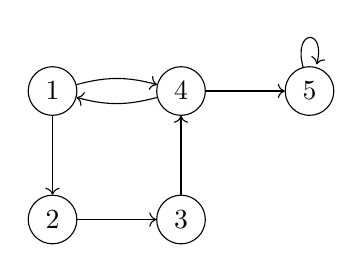
\begin{tikzpicture}[->]
            \node[draw, circle] (1) {1};
            \node[draw, circle, below=of 1] (2) {2};
            \node[draw, circle, right=of 2] (3) {3};
            \node[draw, circle, above=of 3] (4) {4};
            \node[draw, circle, right=of 4] (5) {5};

            %\draw[->] (1) to[bend left=15] (4);
            %\draw[->] (4) to[bend left=15] (1);
            %\draw[->] (1) to (2);
            %\draw[->] (2) to (3);
            %\draw[->] (3) to (4);
            %\draw[->] (4) to (5);

            \path (1) edge[bend left=15] (4);
            \path (4) edge[bend left=15] (1);
            \path (1) edge (2);
            \path (2) edge (3);
            \path (3) edge (4);
            \path (4) edge (5);
            \path (5) edge[loop above] (5);
        \end{tikzpicture}
    \end{center}
\end{defi}

\begin{defi}{Ungerichteter Graph}
    Ein \emph{ungerichteter Graph} $G = (V, E)$ besteht aus
    \begin{itemize}
        \item einer endlichen, nicht leeren Menge $V = \{v_1, \ldots, v_n\}$ von \emph{Knoten (vertices)} und
        \item einer symmetrischen Relation $E \subseteq V \times V$ von geordneten Paaren $e = (u, v) \iff (v, u)$ den \emph{Kanten (edges)}.
    \end{itemize}

    Jede Kante $(u,v) \in E$ hat einen Anfangsknoten $u$ und einen Enknoten $v$ und damit eine Richtung von $u$ nach $v$ ($u=v$ ist möglich).

    \vspace{1em}
    \begin{center}
        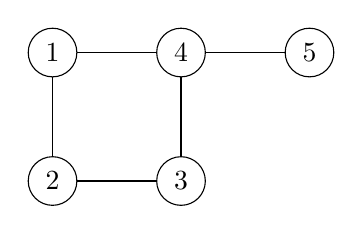
\begin{tikzpicture}
            \node[draw, circle] (1) {1};
            \node[draw, circle, below=of 1] (2) {2};
            \node[draw, circle, right=of 2] (3) {3};
            \node[draw, circle, above=of 3] (4) {4};
            \node[draw, circle, right=of 4] (5) {5};

            %\draw[->] (1) to[bend left=15] (4);
            %\draw[->] (4) to[bend left=15] (1);
            %\draw[->] (1) to (2);
            %\draw[->] (2) to (3);
            %\draw[->] (3) to (4);
            %\draw[->] (4) to (5);

            \path (1) edge (4);
            \path (1) edge (2);
            \path (2) edge (3);
            \path (3) edge (4);
            \path (4) edge (5);
        \end{tikzpicture}
    \end{center}
\end{defi}

\begin{defi}{Gewichteter Graph}
    Ein Graph heißt \emph{gewichtet}, wenn jeder Kante ein Wert als \emph{Gewicht} zugeordnet ist (z.B. Transportkosten, Entfernung).

    \begin{center}
        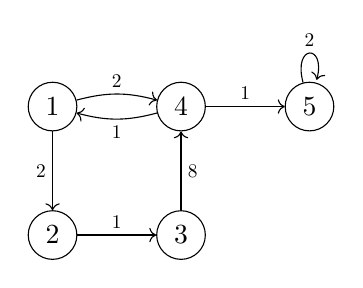
\begin{tikzpicture}[->]
            \node[draw, circle] (1) {1};
            \node[draw, circle, below=of 1] (2) {2};
            \node[draw, circle, right=of 2] (3) {3};
            \node[draw, circle, above=of 3] (4) {4};
            \node[draw, circle, right=of 4] (5) {5};

            %\draw[->] (1) to[bend left=15] (4);
            %\draw[->] (4) to[bend left=15] (1);
            %\draw[->] (1) to (2);
            %\draw[->] (2) to (3);
            %\draw[->] (3) to (4);
            %\draw[->] (4) to (5);

            \path (1) edge[bend left=15] node[above,scale=0.7] {2} (4);
            \path (4) edge[bend left=15] node[below,scale=0.7] {1} (1);
            \path (1) edge node[left,scale=0.7] {2} (2);
            \path (2) edge node[above,scale=0.7] {1} (3);
            \path (3) edge node[right,scale=0.7] {8} (4);
            \path (4) edge node[above,scale=0.7] {1} (5);
            \path (5) edge[loop above] node[above,scale=0.7] {2} (5);
        \end{tikzpicture}
    \end{center}
\end{defi}

\begin{defi}{Teilgraph}
    $G' = (V', E')$ heißt \emph{Teilgraph} von $G=(V, E)$, wenn gilt:
    $$
        V' \subseteq V \quad \text{und} \quad E' \subseteq E
    $$
\end{defi}

\begin{defi}{Weg}
    Sei $G = (V, E)$ ein Graph.

    Eine Folge von Knoten
    $$
        W := (v_1, v_2, \ldots, v_n)
    $$
    heißt \emph{Weg} oder \emph{Pfad} in $G$, falls gilt:
    $$
        \forall 1 \leq i \leq n-1 : (v_i, v_{i+1}) \in E
    $$
    (also eine Folge von zusammenhängenden Kanten)

    $\alpha(W) := v_1$ heißt \emph{Anfangsknoten} des Weges $W$.

    $\omega(W) := v_n$ heißt \emph{Endknoten} des Weges $W$.

    $\forall v_i \in V : (v_i)$ heißt \emph{trivialer Weg} und ist stets ein Weg in $G$.

    Die \emph{Länge eines Weges} ist $l(W) := n-1$, falls $n$ Knoten auf diesem Weg besucht werden.

    Ein Weg heißt \emph{einfacher Weg}, wenn kein Knoten (ausgenommen Start- und Endknoten) mehr als einmal vorkommt.

    Ein \emph{Zykel} oder \emph{Kreis} ist ein nicht-trivialer einfacher Weg mit der Bedingung $\alpha(W) = \omega(W)$.
\end{defi}

\begin{defi}{Adjazenz}
    Zwei Knoten heißen \emph{adjazent (benachbart)}, wenn sie eine Kante verbindet.
\end{defi}

\begin{defi}{Speicherung von Graphen}
    \begin{itemize}
        \item Kantenorientiert
              \begin{itemize}
                  \item Index für Kanten
                  \item für jede Kante speichern: Vorgänger-, Nachfolgerknoten (Markierung, Gewicht)
                  \item meist statische Darstellung, z.B. Kantenliste
              \end{itemize}
        \item Knotenorientiert
              \begin{itemize}
                  \item gebräuchlicher als kantenorientiert
                  \item in vielen Ausprägungen, z.B. Knotenliste, Adjazenzmatrix, Adjazenzliste
                  \item für Adjazenzmatrix gilt:
                        $$
                            A_{ij} = \begin{cases}
                                1 & \text{, falls} \ (i, j) \in E \\
                                0 & \text{, sonst}
                            \end{cases}
                        $$
              \end{itemize}
    \end{itemize}
\end{defi}

\begin{example}{Kantenliste}
    \begin{center}
        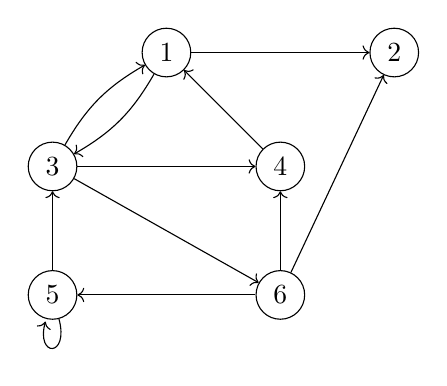
\begin{tikzpicture}[->]
            \node[draw, circle] (1) {1};
            \node[draw, circle, below left=of 1] (3) {3};
            \node[draw, circle, below right=of 1] (4) {4};
            \node[draw, circle, above right=of 4] (2) {2};
            \node[draw, circle, below=of 3] (5) {5};
            \node[draw, circle, below=of 4] (6) {6};

            \path (5) edge[loop below] (5);
            \path (1) edge[bend left=15] (3);
            \path (3) edge[bend left=15] (1);
            \path (4) edge (1);
            \path (1) edge (2);
            \path (3) edge (4);
            \path (5) edge (3);
            \path (3) edge (6);
            \path (6) edge (4);
            \path (6) edge (5);
            \path (6) edge (2);
        \end{tikzpicture}
    \end{center}

    Für eine Kantenliste gilt:
    \begin{itemize}
        \item Position \texttt{0}: Anzahl der Knoten
        \item Position \texttt{1}: Anzahl der Kanten
        \item Danach für jede Kante \texttt{c = (i, j)}:
              \begin{itemize}
                  \item Startknoten \texttt{i}
                  \item Endknoten \texttt{j}
              \end{itemize}
    \end{itemize}

    Für den Graphen $G$ oben gilt die Kantenliste:

    \centering

    \texttt{[6,11,1,2,1,3,3,1,4,1,3,4,3,6,5,3,5,5,6,5,6,2,6,4]}

\end{example}

\begin{example}{Knotenliste}
    \begin{center}
        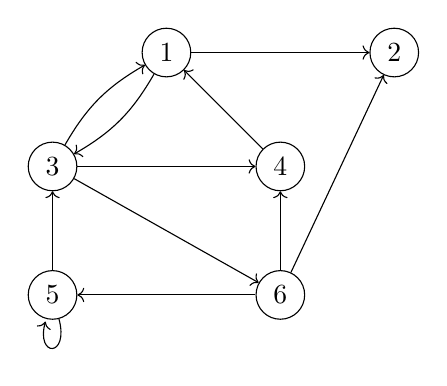
\begin{tikzpicture}[->]
            \node[draw, circle] (1) {1};
            \node[draw, circle, below left=of 1] (3) {3};
            \node[draw, circle, below right=of 1] (4) {4};
            \node[draw, circle, above right=of 4] (2) {2};
            \node[draw, circle, below=of 3] (5) {5};
            \node[draw, circle, below=of 4] (6) {6};

            \path (5) edge[loop below] (5);
            \path (1) edge[bend left=15] (3);
            \path (3) edge[bend left=15] (1);
            \path (4) edge (1);
            \path (1) edge (2);
            \path (3) edge (4);
            \path (5) edge (3);
            \path (3) edge (6);
            \path (6) edge (4);
            \path (6) edge (5);
            \path (6) edge (2);
        \end{tikzpicture}
    \end{center}

    Für eine Knoten gilt:
    \begin{itemize}
        \item Position \texttt{0}: Anzahl der Knoten
        \item Position \texttt{1}: Anzahl der Kanten
        \item Danach für jeden Knoten \texttt{i}:
              \begin{itemize}
                  \item Ausgangsgrad des Knotens \texttt{i} (Anzahl der ausgehenden Kanten)
                  \item Alle Knoten \texttt{j} für die gilt $(i, j) \in E$
              \end{itemize}
    \end{itemize}

    Für den Graphen $G$ oben gilt die Knotenliste:

    \centering

    \texttt{[6,11,2,2,3,0,3,1,4,6,1,1,2,3,5,3,2,4,5]}

\end{example}

\begin{example}{Adjazenzmatrix}
    \begin{center}
        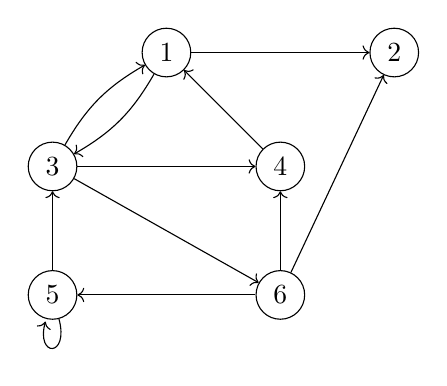
\begin{tikzpicture}[->]
            \node[draw, circle] (1) {1};
            \node[draw, circle, below left=of 1] (3) {3};
            \node[draw, circle, below right=of 1] (4) {4};
            \node[draw, circle, above right=of 4] (2) {2};
            \node[draw, circle, below=of 3] (5) {5};
            \node[draw, circle, below=of 4] (6) {6};

            \path (5) edge[loop below] (5);
            \path (1) edge[bend left=15] (3);
            \path (3) edge[bend left=15] (1);
            \path (4) edge (1);
            \path (1) edge (2);
            \path (3) edge (4);
            \path (5) edge (3);
            \path (3) edge (6);
            \path (6) edge (4);
            \path (6) edge (5);
            \path (6) edge (2);
        \end{tikzpicture}
    \end{center}

    Für den Graphen $G$ oben gilt die Adjazenzmatrix:
    $$
        A(G) = \vektor{
            0 & 1 & 1 & 0 & 0 & 0 \\
            0 & 0 & 0 & 0 & 0 & 0 \\
            1 & 0 & 0 & 1 & 0 & 1 \\
            1 & 0 & 0 & 0 & 0 & 0 \\
            0 & 0 & 1 & 0 & 1 & 0 \\
            0 & 1 & 0 & 1 & 1 & 0
        }
    $$
\end{example}

\begin{example}{Adjazenzliste}
    \begin{center}
        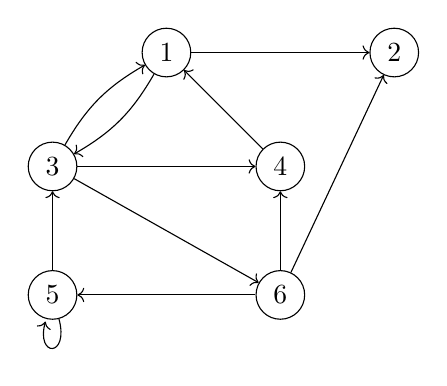
\begin{tikzpicture}[->]
            \node[draw, circle] (1) {1};
            \node[draw, circle, below left=of 1] (3) {3};
            \node[draw, circle, below right=of 1] (4) {4};
            \node[draw, circle, above right=of 4] (2) {2};
            \node[draw, circle, below=of 3] (5) {5};
            \node[draw, circle, below=of 4] (6) {6};

            \path (5) edge[loop below] (5);
            \path (1) edge[bend left=15] (3);
            \path (3) edge[bend left=15] (1);
            \path (4) edge (1);
            \path (1) edge (2);
            \path (3) edge (4);
            \path (5) edge (3);
            \path (3) edge (6);
            \path (6) edge (4);
            \path (6) edge (5);
            \path (6) edge (2);
        \end{tikzpicture}
    \end{center}

    Für den Graphen $G$ oben gilt die Adjazenzliste:

    \vspace{1em}

    \begin{center}
        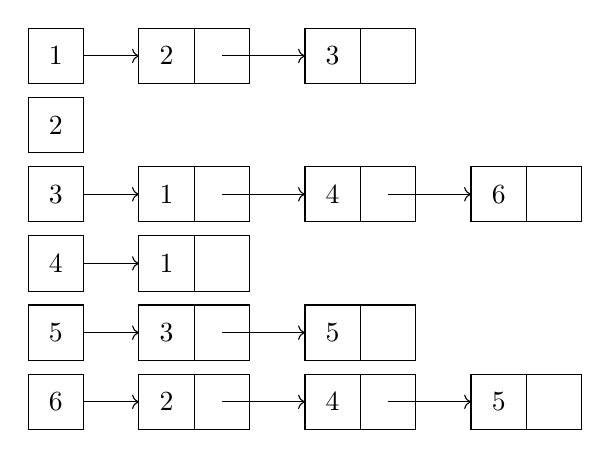
\begin{tikzpicture}[
            start chain = going below,
            StackBlock/.style={minimum width=2em, minimum height=2em, outer sep=0pt, on chain},
            every node/.style={draw, label distance=0.5em},
            node distance=0em
            ]
            {
            \node [StackBlock] (k1) {$1$};
            \node [StackBlock,yshift=-0.5em] (k2) {$2$};
            \node [StackBlock,yshift=-0.5em] (k3) {$3$};
            \node [StackBlock,yshift=-0.5em] (k4) {$4$};
            \node [StackBlock,yshift=-0.5em] (k5) {$5$};
            \node [StackBlock,yshift=-0.5em] (k6) {$6$};

            % Chain 1
            { [continue chain = going right]
            \chainin (k1);

            \node [StackBlock, xshift=2em] (12) {$2$};
            \node [StackBlock] (12p) {};
            \node [StackBlock, xshift=2em] (13) {$3$};
            \node [StackBlock] (13p) {};
            }

            % Chain 3
            { [continue chain = going right]
            \chainin (k3);

            \node [StackBlock, xshift=2em] (31) {$1$};
            \node [StackBlock] (31p) {};
            \node [StackBlock, xshift=2em] (34) {$4$};
            \node [StackBlock] (34p) {};
            \node [StackBlock, xshift=2em] (36) {$6$};
            \node [StackBlock] (36p) {};
            }

            % Chain 4
            { [continue chain = going right]
            \chainin (k4);

            \node [StackBlock, xshift=2em] (41) {$1$};
            \node [StackBlock] (41p) {};
            }

            % Chain 5
            { [continue chain = going right]
            \chainin (k5);

            \node [StackBlock, xshift=2em] (53) {$3$};
            \node [StackBlock] (53p) {};
            \node [StackBlock, xshift=2em] (55) {$5$};
            \node [StackBlock] (55p) {};
            }

            % Chain 6
            { [continue chain = going right]
            \chainin (k6);

            \node [StackBlock, xshift=2em] (62) {$2$};
            \node [StackBlock] (62p) {};
            \node [StackBlock, xshift=2em] (64) {$4$};
            \node [StackBlock] (64p) {};
            \node [StackBlock, xshift=2em] (65) {$5$};
            \node [StackBlock] (65p) {};
            }

            \draw[->] (k1.east) [out=0, in=180] to (12.west);
            \draw[->] (k3.east) [out=0, in=180] to (31.west);
            \draw[->] (k4.east) [out=0, in=180] to (41.west);
            \draw[->] (k5.east) [out=0, in=180] to (53.west);
            \draw[->] (k6.east) [out=0, in=180] to (62.west);

            \draw[->] (12p.center) [out=0, in=180] to (13.west);

            \draw[->] (31p.center) [out=0, in=180] to (34.west);
            \draw[->] (34p.center) [out=0, in=180] to (36.west);

            \draw[->] (53p.center) [out=0, in=180] to (55.west);

            \draw[->] (62p.center) [out=0, in=180] to (64.west);
            \draw[->] (64p.center) [out=0, in=180] to (65.west);
            }
        \end{tikzpicture}
    \end{center}
\end{example}

\subsection{Suche}

\begin{algo}{Breitensuche}
    \begin{enumerate}
        \item Zunächst werden alle Knoten als \glqq noch nicht besucht\grqq markiert.
        \item Startpunkt $v$ wählen und als \glqq besucht\grqq markieren.
        \item Jetzt:
              \begin{enumerate}
                  \item alle von $v$ aus direkt erreichbaren (nicht besuchten) Knoten \glqq besuchen\grqq
                  \item alle von $v$ über zwei Kanten erreichbaren (nicht besuchten) Knoten \glqq besuchen\grqq
                  \item $\ldots$
              \end{enumerate}
        \item Wenn noch nicht alle Knoten besucht worden sind, wähle einen neuen unbesuchten Startpunkt $v$ und beginne bei Schritt 3
    \end{enumerate}

    Start bei Knoten 1.

    \begin{center}
        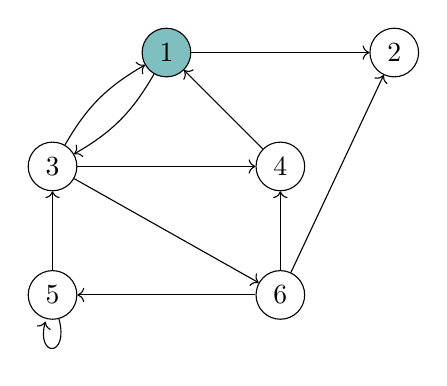
\begin{tikzpicture}[->]
            \node[draw, circle, current] (1) {1};
            \node[draw, circle, below left=of 1] (3) {3};
            \node[draw, circle, below right=of 1] (4) {4};
            \node[draw, circle, above right=of 4] (2) {2};
            \node[draw, circle, below=of 3] (5) {5};
            \node[draw, circle, below=of 4] (6) {6};

            \path (5) edge[loop below] (5);
            \path (1) edge[bend left=15] (3);
            \path (3) edge[bend left=15] (1);
            \path (4) edge (1);
            \path (1) edge (2);
            \path (3) edge (4);
            \path (5) edge (3);
            \path (3) edge (6);
            \path (6) edge (4);
            \path (6) edge (5);
            \path (6) edge (2);
        \end{tikzpicture}
        %
        \hspace{5em}
        %
        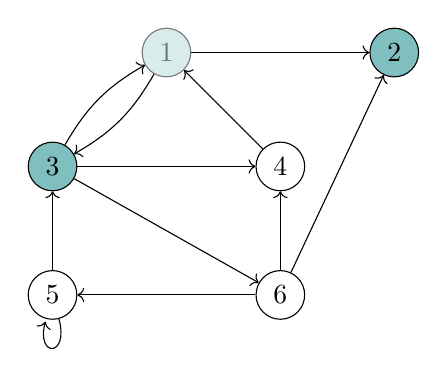
\begin{tikzpicture}[->]
            \node[draw, circle, visited] (1) {1};
            \node[draw, circle, below left=of 1, current] (3) {3};
            \node[draw, circle, below right=of 1] (4) {4};
            \node[draw, circle, above right=of 4, current] (2) {2};
            \node[draw, circle, below=of 3] (5) {5};
            \node[draw, circle, below=of 4] (6) {6};

            \path (5) edge[loop below] (5);
            \path (1) edge[bend left=15] (3);
            \path (3) edge[bend left=15] (1);
            \path (4) edge (1);
            \path (1) edge (2);
            \path (3) edge (4);
            \path (5) edge (3);
            \path (3) edge (6);
            \path (6) edge (4);
            \path (6) edge (5);
            \path (6) edge (2);
        \end{tikzpicture}
        %
        %\hspace{5em}
        %
        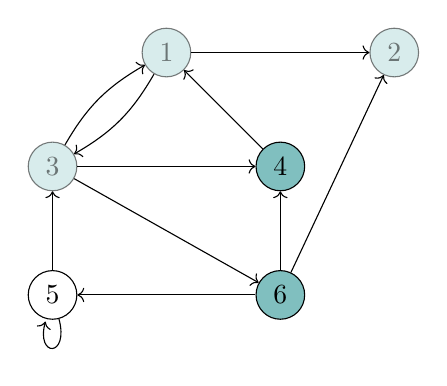
\begin{tikzpicture}[->]
            \node[draw, circle, visited] (1) {1};
            \node[draw, circle, below left=of 1, visited] (3) {3};
            \node[draw, circle, below right=of 1, current] (4) {4};
            \node[draw, circle, above right=of 4, visited] (2) {2};
            \node[draw, circle, below=of 3] (5) {5};
            \node[draw, circle, below=of 4, current] (6) {6};

            \path (5) edge[loop below] (5);
            \path (1) edge[bend left=15] (3);
            \path (3) edge[bend left=15] (1);
            \path (4) edge (1);
            \path (1) edge (2);
            \path (3) edge (4);
            \path (5) edge (3);
            \path (3) edge (6);
            \path (6) edge (4);
            \path (6) edge (5);
            \path (6) edge (2);
        \end{tikzpicture}
        %
        \hspace{5em}
        %
        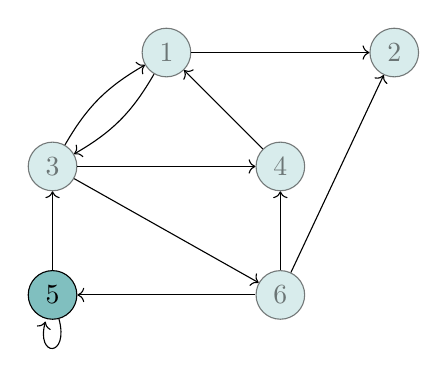
\begin{tikzpicture}[->]
            \node[draw, circle, visited] (1) {1};
            \node[draw, circle, below left=of 1, visited] (3) {3};
            \node[draw, circle, below right=of 1, visited] (4) {4};
            \node[draw, circle, above right=of 4, visited] (2) {2};
            \node[draw, circle, below=of 3, current] (5) {5};
            \node[draw, circle, below=of 4, visited] (6) {6};

            \path (5) edge[loop below] (5);
            \path (1) edge[bend left=15] (3);
            \path (3) edge[bend left=15] (1);
            \path (4) edge (1);
            \path (1) edge (2);
            \path (3) edge (4);
            \path (5) edge (3);
            \path (3) edge (6);
            \path (6) edge (4);
            \path (6) edge (5);
            \path (6) edge (2);
        \end{tikzpicture}
        %
        %\hspace{5em}
        %
        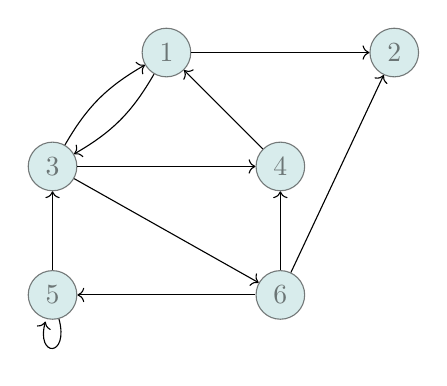
\begin{tikzpicture}[->]
            \node[draw, circle, visited] (1) {1};
            \node[draw, circle, below left=of 1, visited] (3) {3};
            \node[draw, circle, below right=of 1, visited] (4) {4};
            \node[draw, circle, above right=of 4, visited] (2) {2};
            \node[draw, circle, below=of 3, visited] (5) {5};
            \node[draw, circle, below=of 4, visited] (6) {6};

            \path (5) edge[loop below] (5);
            \path (1) edge[bend left=15] (3);
            \path (3) edge[bend left=15] (1);
            \path (4) edge (1);
            \path (1) edge (2);
            \path (3) edge (4);
            \path (5) edge (3);
            \path (3) edge (6);
            \path (6) edge (4);
            \path (6) edge (5);
            \path (6) edge (2);
        \end{tikzpicture}
    \end{center}
\end{algo}

\begin{algo}{Tiefensuche}
    \begin{enumerate}
        \item Zunächst alle Knoten als \glqq noch nicht besucht\grqq markieren.
        \item Startpunkt $v$ wählen und als \glqq besucht\grqq markieren.
        \item Von dort aus möglichst langen Pfad entlang gehen; dabei nur bisher nicht besuchte Knoten \glqq besuchen\grqq
        \item Wenn dann noch nicht alle Knoten besucht worden sind, wähle einen neuen unbesuchten Startpunkt $v$ und beginne bei Schritt 3
    \end{enumerate}

    Start bei Knoten 1.

    \begin{center}
        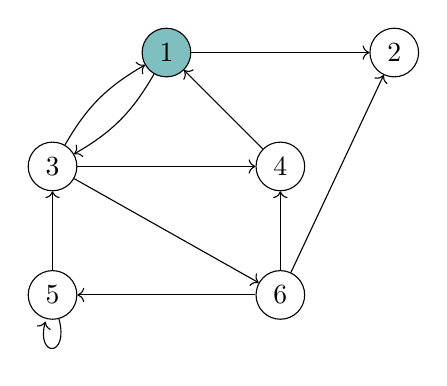
\begin{tikzpicture}[->]
            \node[draw, circle, current] (1) {1};
            \node[draw, circle, below left=of 1] (3) {3};
            \node[draw, circle, below right=of 1] (4) {4};
            \node[draw, circle, above right=of 4] (2) {2};
            \node[draw, circle, below=of 3] (5) {5};
            \node[draw, circle, below=of 4] (6) {6};

            \path (5) edge[loop below] (5);
            \path (1) edge[bend left=15] (3);
            \path (3) edge[bend left=15] (1);
            \path (4) edge (1);
            \path (1) edge (2);
            \path (3) edge (4);
            \path (5) edge (3);
            \path (3) edge (6);
            \path (6) edge (4);
            \path (6) edge (5);
            \path (6) edge (2);
        \end{tikzpicture}
        %
        \hspace{5em}
        %
        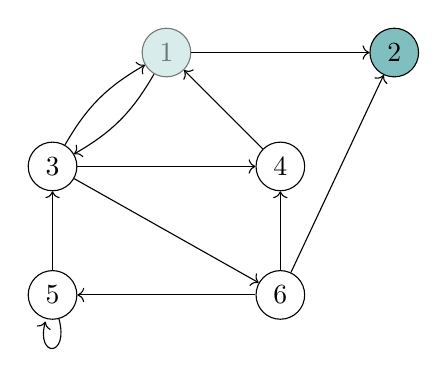
\begin{tikzpicture}[->]
            \node[draw, circle, visited] (1) {1};
            \node[draw, circle, below left=of 1] (3) {3};
            \node[draw, circle, below right=of 1] (4) {4};
            \node[draw, circle, above right=of 4, current] (2) {2};
            \node[draw, circle, below=of 3] (5) {5};
            \node[draw, circle, below=of 4] (6) {6};

            \path (5) edge[loop below] (5);
            \path (1) edge[bend left=15] (3);
            \path (3) edge[bend left=15] (1);
            \path (4) edge (1);
            \path (1) edge (2);
            \path (3) edge (4);
            \path (5) edge (3);
            \path (3) edge (6);
            \path (6) edge (4);
            \path (6) edge (5);
            \path (6) edge (2);
        \end{tikzpicture}
        %
        %\hspace{5em}
        %
        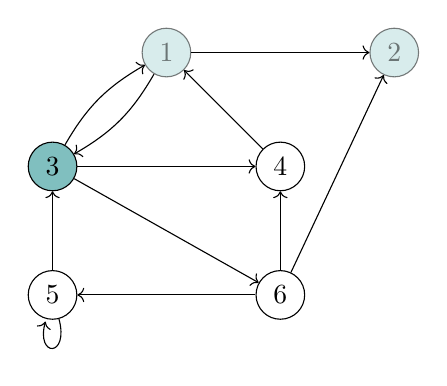
\begin{tikzpicture}[->]
            \node[draw, circle, visited] (1) {1};
            \node[draw, circle, below left=of 1, current] (3) {3};
            \node[draw, circle, below right=of 1] (4) {4};
            \node[draw, circle, above right=of 4, visited] (2) {2};
            \node[draw, circle, below=of 3] (5) {5};
            \node[draw, circle, below=of 4] (6) {6};

            \path (5) edge[loop below] (5);
            \path (1) edge[bend left=15] (3);
            \path (3) edge[bend left=15] (1);
            \path (4) edge (1);
            \path (1) edge (2);
            \path (3) edge (4);
            \path (5) edge (3);
            \path (3) edge (6);
            \path (6) edge (4);
            \path (6) edge (5);
            \path (6) edge (2);
        \end{tikzpicture}
        %
        \hspace{5em}
        %
        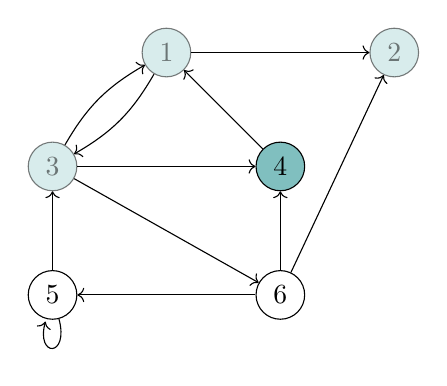
\begin{tikzpicture}[->]
            \node[draw, circle, visited] (1) {1};
            \node[draw, circle, below left=of 1, visited] (3) {3};
            \node[draw, circle, below right=of 1, current] (4) {4};
            \node[draw, circle, above right=of 4, visited] (2) {2};
            \node[draw, circle, below=of 3] (5) {5};
            \node[draw, circle, below=of 4] (6) {6};

            \path (5) edge[loop below] (5);
            \path (1) edge[bend left=15] (3);
            \path (3) edge[bend left=15] (1);
            \path (4) edge (1);
            \path (1) edge (2);
            \path (3) edge (4);
            \path (5) edge (3);
            \path (3) edge (6);
            \path (6) edge (4);
            \path (6) edge (5);
            \path (6) edge (2);
        \end{tikzpicture}
        %
        %\hspace{5em}
        %
        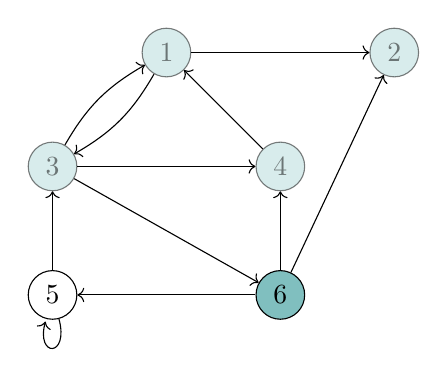
\begin{tikzpicture}[->]
            \node[draw, circle, visited] (1) {1};
            \node[draw, circle, below left=of 1, visited] (3) {3};
            \node[draw, circle, below right=of 1, visited] (4) {4};
            \node[draw, circle, above right=of 4, visited] (2) {2};
            \node[draw, circle, below=of 3] (5) {5};
            \node[draw, circle, below=of 4, current] (6) {6};

            \path (5) edge[loop below] (5);
            \path (1) edge[bend left=15] (3);
            \path (3) edge[bend left=15] (1);
            \path (4) edge (1);
            \path (1) edge (2);
            \path (3) edge (4);
            \path (5) edge (3);
            \path (3) edge (6);
            \path (6) edge (4);
            \path (6) edge (5);
            \path (6) edge (2);
        \end{tikzpicture}
        %
        \hspace{5em}
        %
        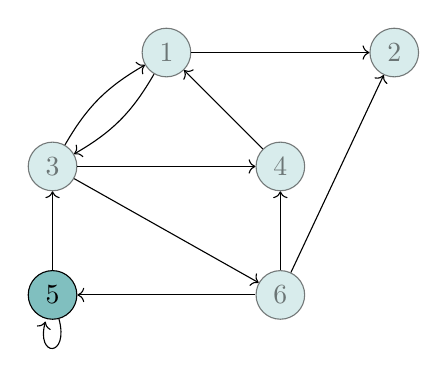
\begin{tikzpicture}[->]
            \node[draw, circle, visited] (1) {1};
            \node[draw, circle, below left=of 1, visited] (3) {3};
            \node[draw, circle, below right=of 1, visited] (4) {4};
            \node[draw, circle, above right=of 4, visited] (2) {2};
            \node[draw, circle, below=of 3, current] (5) {5};
            \node[draw, circle, below=of 4, visited] (6) {6};

            \path (5) edge[loop below] (5);
            \path (1) edge[bend left=15] (3);
            \path (3) edge[bend left=15] (1);
            \path (4) edge (1);
            \path (1) edge (2);
            \path (3) edge (4);
            \path (5) edge (3);
            \path (3) edge (6);
            \path (6) edge (4);
            \path (6) edge (5);
            \path (6) edge (2);
        \end{tikzpicture}
        %
        %\hspace{5em}
        %
        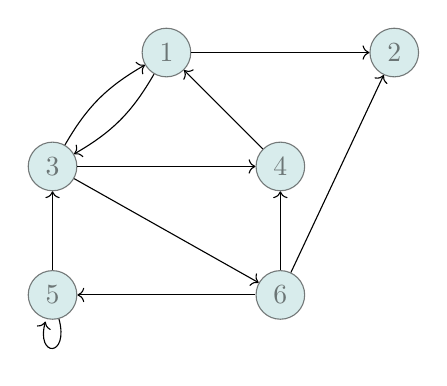
\begin{tikzpicture}[->]
            \node[draw, circle, visited] (1) {1};
            \node[draw, circle, below left=of 1, visited] (3) {3};
            \node[draw, circle, below right=of 1, visited] (4) {4};
            \node[draw, circle, above right=of 4, visited] (2) {2};
            \node[draw, circle, below=of 3, visited] (5) {5};
            \node[draw, circle, below=of 4, visited] (6) {6};

            \path (5) edge[loop below] (5);
            \path (1) edge[bend left=15] (3);
            \path (3) edge[bend left=15] (1);
            \path (4) edge (1);
            \path (1) edge (2);
            \path (3) edge (4);
            \path (5) edge (3);
            \path (3) edge (6);
            \path (6) edge (4);
            \path (6) edge (5);
            \path (6) edge (2);
        \end{tikzpicture}
    \end{center}
\end{algo}

\begin{defi}{Level-Order-Baumdurchlauf}
    Führt man eine Breitensuche bei Bäumen aus, stellt man fest:
    \begin{itemize}
        \item Es ist nicht nötig, die Knoten zu markieren.
        \item Der Baum wird Ebene für Ebene durchlaufen,
    \end{itemize}

    Diesen Durchlauf nennt man \emph{Level-Order-Durchlauf}.
\end{defi}

\begin{defi}{Pre-Order-Baumdurchlauf}
    Führt man eine Tiefensuche bei Bäumen aus, nennt man diesen Durchlauf \emph{Pre-Order-Durchlauf}.

    Dabei wird stets der linke Teilbaum zuerst durchlaufen.
\end{defi}

\begin{defi}{Post-Order-Baumdurchlauf}
    \begin{enumerate}
        \item Durchlaufe linken Teilbaum
        \item Durchlaufe rechten Teilbaum
        \item Betrachte die Wurzel
    \end{enumerate}
\end{defi}

\begin{defi}{In-Order-Baumdurchlauf}
    \begin{enumerate}
        \item Durchlaufe linken Teilbaum
        \item Betrachte die Wurzel
        \item Durchlaufe rechten Teilbaum
    \end{enumerate}
\end{defi}

\begin{example}{Baumdurchläufe}
    \begin{center}
        \begin{forest}
            baseline,anchor=north,
            for tree={circle, draw,
                    minimum size=2em, % <-- added
                    inner sep=1pt}
                [
                    45
                        [
                            36
                                [
                                    25
                                        [
                                            2
                                        ]
                                        [
                                            3
                                        ]
                                ]
                                [
                                    26
                                        [
                                            19
                                        ]
                                        [, draw=none, edge={draw=none}]
                                ]
                        ]
                        [
                            17
                                [
                                    7
                                ]
                                [
                                    1
                                ]
                        ]
                ]
        \end{forest}
    \end{center}

    Für den gegebenen Baum gelten folgende Baumdurchläufe:

    \centering
    \begin{tabular}{|l|cccccccccc|}
        \hline
        Pre-Order   & 45 & 36 & 25 & 2  & 3  & 26 & 19 & 17 & 7  & 1  \\
        \hline
        In-Order    & 2  & 25 & 3  & 19 & 26 & 36 & 45 & 7  & 17 & 1  \\
        \hline
        Post-Order  & 2  & 3  & 25 & 19 & 26 & 36 & 7  & 1  & 17 & 45 \\
        \hline
        Level-Order & 45 & 36 & 17 & 25 & 26 & 7  & 1  & 2  & 3  & 19 \\
        \hline
    \end{tabular}
\end{example}


\subsection{Entwurfsprinzipien}

\begin{defi}{Traveling-Salesman-Problem}
    Das \emph{Traveling-Salesman-Problem} ist ein Optimierungsproblem.
    Die Aufgabe besteht darin, eine Reihenfolge für den Besuch mehrerer Orte so zu wählen, dass:
    \begin{itemize}
        \item kein Ort doppelt besucht wird und
        \item die Reisestrecke minimal ist.
    \end{itemize}
\end{defi}

\begin{defi}{Greedy}
    Wähle immer den Schritt, desse unmittelbarer Folgezustand das beste Ergebnis liefert.
    Denke nicht an die weiteren Schritte (greedy = gierig).

    Ob ein Greedy-Algorithmus die optimale Lösung liefert oder nicht, ist vom konkreten Problem abhängig.

    Für das Traveling-Salesman-Problem ist eine Greedy-Lösung z.B. die \emph{Nearest-Neighbour-Lösung}:
    \begin{itemize}
        \item Gehe in jedem Schritt zur nächstliegenden Stadt, die noch nicht besucht ist.
        \item $\bigo(n^2)$
        \item liefert nicht die optimale Lösung (kann sogar beliebig schlecht werden)
        \item arbeitet meistens einigermaßen gut
    \end{itemize}
\end{defi}

\begin{bonus}{Random Insertion}
    Wähle immer einen zufälligen Knoten.

    \begin{itemize}
        \item $\bigo(n^2)$
        \item keine Garantie, dass die Lösung irgendeinem Gütekriterium genügt
        \item im Allgmeinen ist Lösung ziemlich gut
        \item Vorteil: Durch den Zufallsfaktor kann man das Verfahren beliebig oft wiederholen und sich die beste Lösung heraussuchen.
    \end{itemize}
\end{bonus}

\begin{bonus}{Lösung mit minimalem Spannbaum}
    \begin{enumerate}
        \item Konstruktion eines minimalen Spannbaums nach Prim
        \item Durchlaufen mit Tiefensuche
        \item jede Kante wird zweimal durchlaufen
        \item summierte Gewichte des minimalen Spannbaums müssen kleiner sein als das optimale TSP-Ergebnis
        \item Optimierung:
              \begin{itemize}
                  \item Knoten schon einmal besucht: beim nächsten Mal überspringen
                  \item bei einem Schritt mehrere Möglichkeiten: zuerst kürzeren Weg wählen (greedy)
              \end{itemize}
    \end{enumerate}
\end{bonus}

\begin{defi}{Backtracking}
    Durchlauf eines Lösungsbaum in Pre-Order-Reihenfolge.

    Situation: Mehrere Alternativen sind in bestimmten Schritten des Algorithmus möglich.

    Lösung mit \emph{Backtracking}:
    \begin{enumerate}
        \item Wähle eine Alternative und verfolge dieses Weg weiter.
        \item Falls man so eine Lösung des Problems findet, ist man fertig.
        \item Ansonsten gehe einen Schritt zurück und verfolge rekursiv eine andere (nicht versuchte) Alternative in diesem Schritt.
        \item Falls alle Alternativen erfolglos probiert wurden, einen Schritt zurückgehen $\ldots$
    \end{enumerate}

    Backtracking-Algorithmen können exponentiellen Aufwand haben.

    Tipps:
    \begin{itemize}
        \item Durch Einführung von Zusatzbedingungen möglichst viele Sackgassen ausschließen.
        \item Symmetriebedingungen ausnutzen.
    \end{itemize}
\end{defi}

\begin{defi}{Branch and Bound}
    \begin{enumerate}
        \item Ermitteln einer oberen Schranke (greedy)
        \item Falls dieser Wert überschritten wird, kann man die Suche auf diesem Pfad abbrechen.
        \item Bessere Lösungen nutzen, um die Schranke zu verbessern.
    \end{enumerate}
\end{defi}


\subsection{Graphalgorithmen}

\begin{defi}{Bipartiter Graph}
    Ein Graph $G=(V, E)$ heißt \emph{bipartit}, wenn man $V$ in disjunkte Mengen $U$ und $W$ zerlegen kann, so dass alle Kanten zwischen $U$ und $W$ verlaufen.

    Die Knoten eines bipartiten Graphen lassen sich mit zwei Farben so einfärben, dass zwei Nachbarknoten immer unterschiedlich eingefärbt sind.
\end{defi}

\begin{algo}{Prüfung ob ein Graph bipartit ist}
    \begin{enumerate}
        \item Einfärben des 1. Knotens
        \item Durchlauf mit Breitensuche
        \item Abwechselndes Färben
    \end{enumerate}

    Start bei Knoten 1.

    \vspace{1em}

    \begin{center}
        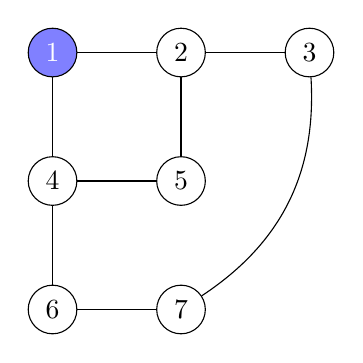
\begin{tikzpicture}
            \node[draw, circle, text=white, fill = blue!50] (1) {1};
            \node[draw, circle, right=of 1] (2) {2};
            \node[draw, circle, right=of 2] (3) {3};
            \node[draw, circle, below=of 1] (4) {4};
            \node[draw, circle, right=of 4] (5) {5};
            \node[draw, circle, below=of 4] (6) {6};
            \node[draw, circle, right=of 6] (7) {7};

            \path (1) edge (2);
            \path (2) edge (3);
            \path (1) edge (4);
            \path (4) edge (5);
            \path (2) edge (5);
            \path (4) edge (6);
            \path (6) edge (7);
            \path (3) edge[bend left=30] (7);
        \end{tikzpicture}
        %
        \hspace{5em}
        %
        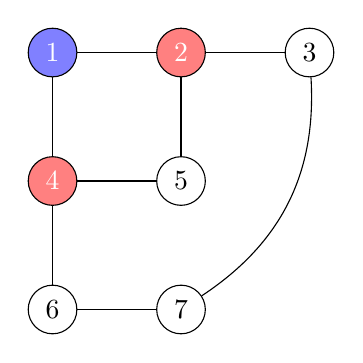
\begin{tikzpicture}
            \node[draw, circle, text=white, fill = blue!50] (1) {1};
            \node[draw, circle, text=white, right=of 1, fill = red!50] (2) {2};
            \node[draw, circle, right=of 2] (3) {3};
            \node[draw, circle, text=white, below=of 1, fill = red!50] (4) {4};
            \node[draw, circle, right=of 4] (5) {5};
            \node[draw, circle, below=of 4] (6) {6};
            \node[draw, circle, right=of 6] (7) {7};

            \path (1) edge (2);
            \path (2) edge (3);
            \path (1) edge (4);
            \path (4) edge (5);
            \path (2) edge (5);
            \path (4) edge (6);
            \path (6) edge (7);
            \path (3) edge[bend left=30] (7);
        \end{tikzpicture}

        \vspace{1em}

        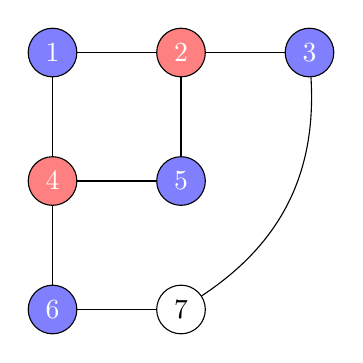
\begin{tikzpicture}
            \node[draw, circle, text=white, fill = blue!50] (1) {1};
            \node[draw, circle, text=white, right=of 1, fill = red!50] (2) {2};
            \node[draw, circle, text=white, right=of 2, fill = blue!50] (3) {3};
            \node[draw, circle, text=white, below=of 1, fill = red!50] (4) {4};
            \node[draw, circle, text=white, right=of 4, fill = blue!50] (5) {5};
            \node[draw, circle, text=white, below=of 4, fill = blue!50] (6) {6};
            \node[draw, circle, right=of 6] (7) {7};

            \path (1) edge (2);
            \path (2) edge (3);
            \path (1) edge (4);
            \path (4) edge (5);
            \path (2) edge (5);
            \path (4) edge (6);
            \path (6) edge (7);
            \path (3) edge[bend left=30] (7);
        \end{tikzpicture}
        %
        \hspace{5em}
        %
        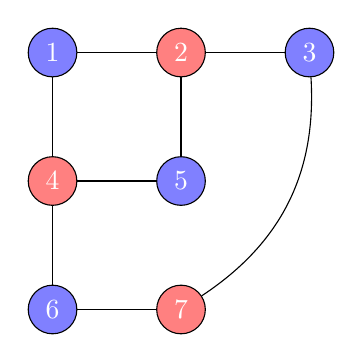
\begin{tikzpicture}
            \node[draw, circle, text=white, fill = blue!50] (1) {1};
            \node[draw, circle, text=white, right=of 1, fill = red!50] (2) {2};
            \node[draw, circle, text=white, right=of 2, fill = blue!50] (3) {3};
            \node[draw, circle, text=white, below=of 1, fill = red!50] (4) {4};
            \node[draw, circle, text=white, right=of 4, fill = blue!50] (5) {5};
            \node[draw, circle, text=white, below=of 4, fill = blue!50] (6) {6};
            \node[draw, circle, text=white, right=of 6, fill = red!50] (7) {7};

            \path (1) edge (2);
            \path (2) edge (3);
            \path (1) edge (4);
            \path (4) edge (5);
            \path (2) edge (5);
            \path (4) edge (6);
            \path (6) edge (7);
            \path (3) edge[bend left=30] (7);
        \end{tikzpicture}
    \end{center}
\end{algo}

\begin{defi}{Spannbaum}
    Ein \emph{Spannbaum} verbindet alle Knoten eines ungerichteten Graphen miteinander, hat jedoch keine Kreise.

    Der \emph{minimale Spannbaum} ist der Spannbaum, dessen Kanten das kleinste summierte Gewicht haben.
\end{defi}

\begin{algo}{Prim-Algorithmus}
    \begin{enumerate}
        \item Wähle einen beliebigen Startknoten für den minimalen Spannbaum $T$
        \item Solange $T$ noch nicht alle Knoten enthält:
              \begin{itemize}
                  \item Wähle eine Kante $e$ mit minimalem Gewicht aus, die einen noch nicht in $T$ enthaltenen Knoten $v$ mit $T$ verbindet.
                  \item Füge $e$ und $v$ dem Graphen $T$ hinzu.
              \end{itemize}
    \end{enumerate}

    Start bei Knoten $A$.

    \vspace{1em}
    \begin{center}
        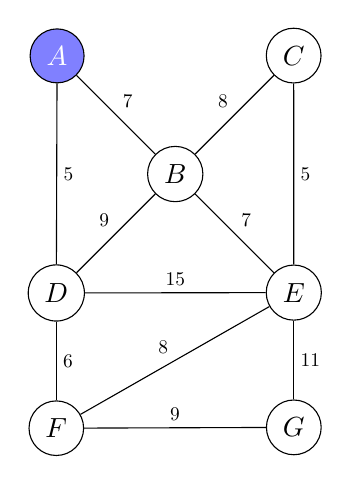
\begin{tikzpicture}
            \node[draw, circle, prim node] (A) {$A$};
            \node[draw, circle, below right=of A] (B) {$B$};
            \node[draw, circle, above right=of B] (C) {$C$};
            \node[draw, circle, below left=of B] (D) {$D$};
            \node[draw, circle, below right=of B] (E) {$E$};
            \node[draw, circle, below=of D] (F) {$F$};
            \node[draw, circle, below=of E] (G) {$G$};

            \path (A) edge node[weight,above right] {7} (B);
            \path (B) edge node[weight,above left] {8} (C);
            \path (D) edge node[weight,right] {5} (A);
            \path (D) edge node[weight,above left] {9} (B);
            \path (E) edge node[weight,above right] {7} (B);
            \path (C) edge node[weight,right] {5} (E);
            \path (D) edge node[weight,above] {15} (E);
            \path (D) edge node[weight,right] {6} (F);
            \path (E) edge node[weight,above left] {8} (F);
            \path (E) edge node[weight,right] {11} (G);
            \path (F) edge node[weight,above] {9} (G);
        \end{tikzpicture}
        %
        \hspace{3em}
        %
        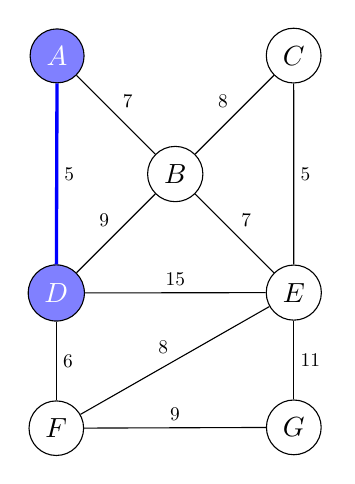
\begin{tikzpicture}
            \node[draw, circle, prim node] (A) {$A$};
            \node[draw, circle, below right=of A] (B) {$B$};
            \node[draw, circle, above right=of B] (C) {$C$};
            \node[draw, circle, below left=of B, prim node] (D) {$D$};
            \node[draw, circle, below right=of B] (E) {$E$};
            \node[draw, circle, below=of D] (F) {$F$};
            \node[draw, circle, below=of E] (G) {$G$};

            \path (A) edge node[weight,above right] {7} (B);
            \path (B) edge node[weight,above left] {8} (C);
            \path (D) edge[prim edge] node[weight,right] {5} (A);
            \path (D) edge node[weight,above left] {9} (B);
            \path (E) edge node[weight,above right] {7} (B);
            \path (C) edge node[weight,right] {5} (E);
            \path (D) edge node[weight,above] {15} (E);
            \path (D) edge node[weight,right] {6} (F);
            \path (E) edge node[weight,above left] {8} (F);
            \path (E) edge node[weight,right] {11} (G);
            \path (F) edge node[weight,above] {9} (G);
        \end{tikzpicture}
        %
        \hspace{3em}
        %
        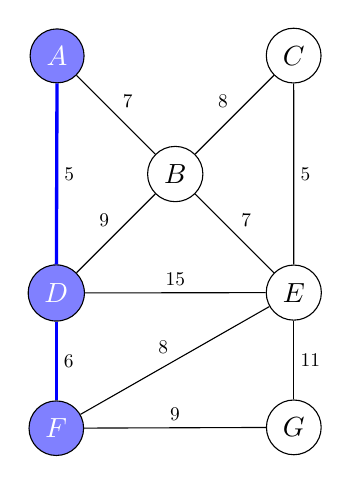
\begin{tikzpicture}
            \node[draw, circle, prim node] (A) {$A$};
            \node[draw, circle, below right=of A] (B) {$B$};
            \node[draw, circle, above right=of B] (C) {$C$};
            \node[draw, circle, below left=of B, prim node] (D) {$D$};
            \node[draw, circle, below right=of B] (E) {$E$};
            \node[draw, circle, below=of D, prim node] (F) {$F$};
            \node[draw, circle, below=of E] (G) {$G$};

            \path (A) edge node[weight,above right] {7} (B);
            \path (B) edge node[weight,above left] {8} (C);
            \path (D) edge[prim edge] node[weight,right] {5} (A);
            \path (D) edge node[weight,above left] {9} (B);
            \path (E) edge node[weight,above right] {7} (B);
            \path (C) edge node[weight,right] {5} (E);
            \path (D) edge node[weight,above] {15} (E);
            \path (D) edge[prim edge] node[weight,right] {6} (F);
            \path (E) edge node[weight,above left] {8} (F);
            \path (E) edge node[weight,right] {11} (G);
            \path (F) edge node[weight,above] {9} (G);
        \end{tikzpicture}
        %
        \vspace{1em}
        %

        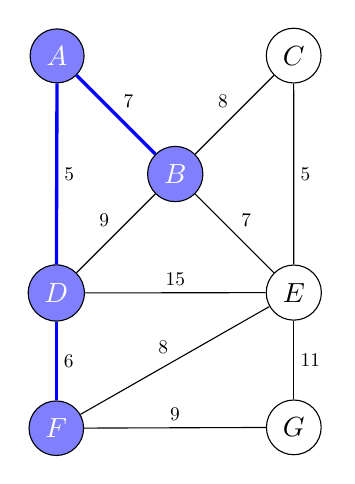
\begin{tikzpicture}
            \node[draw, circle, prim node] (A) {$A$};
            \node[draw, circle, below right=of A, prim node] (B) {$B$};
            \node[draw, circle, above right=of B] (C) {$C$};
            \node[draw, circle, below left=of B, prim node] (D) {$D$};
            \node[draw, circle, below right=of B] (E) {$E$};
            \node[draw, circle, below=of D, prim node] (F) {$F$};
            \node[draw, circle, below=of E] (G) {$G$};

            \path (A) edge[prim edge] node[weight,above right] {7} (B);
            \path (B) edge node[weight,above left] {8} (C);
            \path (D) edge[prim edge] node[weight,right] {5} (A);
            \path (D) edge node[weight,above left] {9} (B);
            \path (E) edge node[weight,above right] {7} (B);
            \path (C) edge node[weight,right] {5} (E);
            \path (D) edge node[weight,above] {15} (E);
            \path (D) edge[prim edge] node[weight,right] {6} (F);
            \path (E) edge node[weight,above left] {8} (F);
            \path (E) edge node[weight,right] {11} (G);
            \path (F) edge node[weight,above] {9} (G);
        \end{tikzpicture}
        %
        \hspace{3em}
        %
        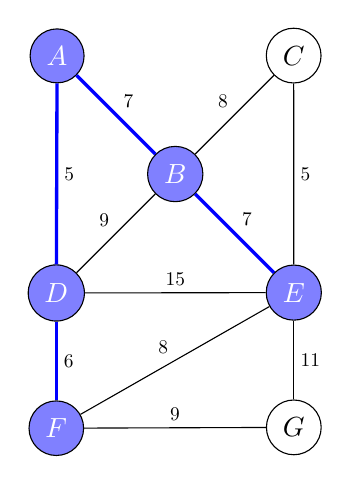
\begin{tikzpicture}
            \node[draw, circle, prim node] (A) {$A$};
            \node[draw, circle, below right=of A, prim node] (B) {$B$};
            \node[draw, circle, above right=of B] (C) {$C$};
            \node[draw, circle, below left=of B, prim node] (D) {$D$};
            \node[draw, circle, below right=of B, prim node] (E) {$E$};
            \node[draw, circle, below=of D, prim node] (F) {$F$};
            \node[draw, circle, below=of E] (G) {$G$};

            \path (A) edge[prim edge] node[weight,above right] {7} (B);
            \path (B) edge node[weight,above left] {8} (C);
            \path (D) edge[prim edge] node[weight,right] {5} (A);
            \path (D) edge node[weight,above left] {9} (B);
            \path (E) edge[prim edge] node[weight,above right] {7} (B);
            \path (C) edge node[weight,right] {5} (E);
            \path (D) edge node[weight,above] {15} (E);
            \path (D) edge[prim edge] node[weight,right] {6} (F);
            \path (E) edge node[weight,above left] {8} (F);
            \path (E) edge node[weight,right] {11} (G);
            \path (F) edge node[weight,above] {9} (G);
        \end{tikzpicture}
        %
        \hspace{3em}
        %
        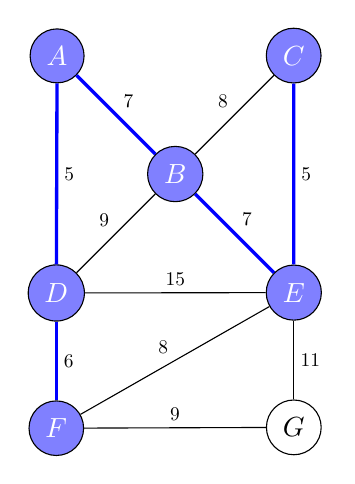
\begin{tikzpicture}
            \node[draw, circle, prim node] (A) {$A$};
            \node[draw, circle, below right=of A, prim node] (B) {$B$};
            \node[draw, circle, above right=of B, prim node] (C) {$C$};
            \node[draw, circle, below left=of B, prim node] (D) {$D$};
            \node[draw, circle, below right=of B, prim node] (E) {$E$};
            \node[draw, circle, below=of D, prim node] (F) {$F$};
            \node[draw, circle, below=of E] (G) {$G$};

            \path (A) edge[prim edge] node[weight,above right] {7} (B);
            \path (B) edge node[weight,above left] {8} (C);
            \path (D) edge[prim edge] node[weight,right] {5} (A);
            \path (D) edge node[weight,above left] {9} (B);
            \path (E) edge[prim edge] node[weight,above right] {7} (B);
            \path (C) edge[prim edge] node[weight,right] {5} (E);
            \path (D) edge node[weight,above] {15} (E);
            \path (D) edge[prim edge] node[weight,right] {6} (F);
            \path (E) edge node[weight,above left] {8} (F);
            \path (E) edge node[weight,right] {11} (G);
            \path (F) edge node[weight,above] {9} (G);
        \end{tikzpicture}
        %
        \vspace{1em}
        %

        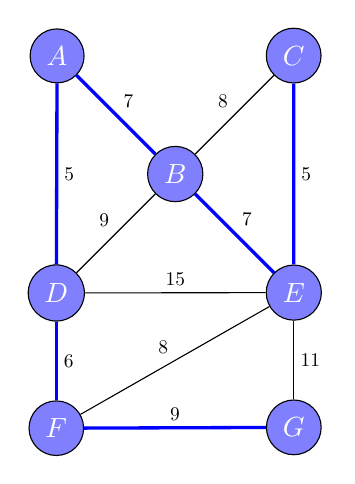
\begin{tikzpicture}
            \node[draw, circle, prim node] (A) {$A$};
            \node[draw, circle, below right=of A, prim node] (B) {$B$};
            \node[draw, circle, above right=of B, prim node] (C) {$C$};
            \node[draw, circle, below left=of B, prim node] (D) {$D$};
            \node[draw, circle, below right=of B, prim node] (E) {$E$};
            \node[draw, circle, below=of D, prim node] (F) {$F$};
            \node[draw, circle, below=of E, prim node] (G) {$G$};

            \path (A) edge[prim edge] node[weight,above right] {7} (B);
            \path (B) edge node[weight,above left] {8} (C);
            \path (D) edge[prim edge] node[weight,right] {5} (A);
            \path (D) edge node[weight,above left] {9} (B);
            \path (E) edge[prim edge] node[weight,above right] {7} (B);
            \path (C) edge[prim edge] node[weight,right] {5} (E);
            \path (D) edge node[weight,above] {15} (E);
            \path (D) edge[prim edge] node[weight,right] {6} (F);
            \path (E) edge node[weight,above left] {8} (F);
            \path (E) edge node[weight,right] {11} (G);
            \path (F) edge[prim edge] node[weight,above] {9} (G);
        \end{tikzpicture}
    \end{center}
\end{algo}

\begin{defi}{Shortest-Path-Probleme}
    Eigentlich: Suche nach \emph{günstigsten Wegen} in gewichteten Graphen: Gewichte $\simeq$ Kosten

    Bei Anwendung auf ungewichtete Graphen ergibt sich: \emph{kürzeste Wege}.

    Beispiele:
    \begin{itemize}
        \item Single-Source-Shortest-Path
              \begin{itemize}
                  \item Dijkstra-Algorithmus (nicht-negative Kantengewichte)
                  \item Bellman-Ford-Algorithmus (keine negativen Zykel)
              \end{itemize}
        \item All-Pairs-Shortest-Path
              \begin{itemize}
                  \item Floyd-Warshall-Algorithmus
              \end{itemize}
        \item One-Pair
              \begin{itemize}
                  \item A*-Algorithmus
              \end{itemize}
    \end{itemize}
\end{defi}

\begin{algo}{Dijkstra-Algorithmus}
    Gegeben: Graph $G = (V, E)$, dessen Bewertungsfunktion die Eigenschaften hat:
    \begin{itemize}
        \item Jede Kante von $v_i$ nach $v_j$ hat nicht-negative Kosten: $C(i, j) \geq 0$
        \item Falls keine Kante zwischen $v_i$ und $v_j$: $C(i, j) = \infty$
        \item Diagonalelemente: $C(i, i) = 0$
    \end{itemize}

    Menge $S$: die Knoten, deren günstigste Wegekosten von der vorgegebenen Quelle (Startknoten) bereits bekannt sind.

    \begin{enumerate}
        \item Initialisierung: $S = \{ \text{Startknoten} \}$
        \item Beginnend mit Quelle alle ausgehenden Kanten betrachten (analog Breitensuche). Nachfolgerknoten $v$ mit günstigster Kante zu $S$ hinzunehmen.
        \item Jetzt: Berechnen, ob die Knoten in $V \setminus S$ günstiger über $v$ als Zwischenweg erreichbar sind, als ohne Umweg über $v$.
        \item Danach: Denjenigen Knoten $v'$ zu $S$ hinzunehmen, der nun am günstigsten zu erreichen ist. Bei zwei gleich günstigen Knoten wird ein beliebiger davon ausgewählt.
        \item Ab Schritt 3 wiederholen, bis alle Knoten in $S$ sind.
    \end{enumerate}

    Zeitkomplexität (bei Speicherung des Graphen mit Adjazenzmatrix): $\bigo(\abs{V}^2)$
\end{algo}

\begin{example}{Dijkstra-Algorithmus}
    \begin{center}
        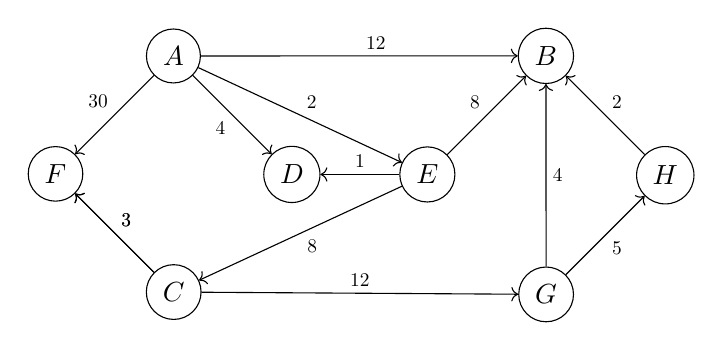
\begin{tikzpicture}[->]
            \node[draw, circle] (A) {$A$};
            \node[draw, circle, below right=of A] (D) {$D$};
            \node[draw, circle, right=of D] (E) {$E$};
            \node[draw, circle, above right=of E] (B) {$B$};
            \node[draw, circle, below right=of B] (H) {$H$};
            \node[draw, circle, below left=of H] (G) {$G$};
            \node[draw, circle, below left=of A] (F) {$F$};
            \node[draw, circle, below right=of F] (C) {$C$};

            \path (A) edge node[weight, below left] {4} (D);
            \path (A) edge node[weight, above right] {2} (E);
            \path (A) edge node[weight, above right] {12} (B);
            \path (A) edge node[weight, above left] {30} (F);
            \path (E) edge node[weight, above] {1} (D);
            \path (E) edge node[weight, below right] {8} (C);
            \path (E) edge node[weight, above left] {8} (B);
            \path (C) edge node[weight, above right] {3} (F);
            \path (C) edge node[weight, above right] {3} (F);
            \path (C) edge node[weight, above] {12} (G);
            \path (G) edge node[weight, right] {4} (B);
            \path (G) edge node[weight, below right] {5} (H);
            \path (H) edge node[weight, above right] {2} (B);
        \end{tikzpicture}

        \vspace{1em}

        \begin{tabular}{|c|ccccccc|ccccccc|}
            \hline
            \multirow{2}{*}{$v_i$} & $d[2]$      & $d[3]$      & $d[4]$     & $d[5]$     & $d[6]$      & $d[7]$      & $d[8]$      & $p[2]$ & $p[3]$ & $p[4]$ & $p[5]$ & $p[6]$ & $p[7]$ & $p[8]$ \\ \cline{2-15}
                                   & B           & C           & D          & E          & F           & G           & H           & B      & C      & D      & E      & F      & G      & H      \\
            \hline
            A                      & 12          &             & 4          & \textbf{2} & 30          &             &             & A      &        & A      & A      & A      &        &        \\
            E                      & 10          & 10          & \textbf{3} & \textbf{2} & 30          &             &             & E      & E      & E      & A      & A      &        &        \\
            D                      & \textbf{10} & 10          & \textbf{3} & \textbf{2} & 30          &             &             & E      & E      & E      & A      & A      &        &        \\
            B                      & \textbf{10} & \textbf{10} & \textbf{3} & \textbf{2} & 30          &             &             & E      & E      & E      & A      & A      &        &        \\
            C                      & \textbf{10} & \textbf{10} & \textbf{3} & \textbf{2} & \textbf{13} & 22          &             & E      & E      & E      & A      & C      & C      &        \\
            F                      & \textbf{10} & \textbf{10} & \textbf{3} & \textbf{2} & \textbf{13} & \textbf{22} &             & E      & E      & E      & A      & C      & C      &        \\
            G                      & \textbf{10} & \textbf{10} & \textbf{3} & \textbf{2} & \textbf{13} & \textbf{22} & \textbf{27} & E      & E      & E      & A      & C      & C      & G      \\
            H                      & \textbf{10} & \textbf{10} & \textbf{3} & \textbf{2} & \textbf{13} & \textbf{22} & \textbf{27} & E      & E      & E      & A      & C      & C      & G      \\
            \hline
        \end{tabular}
    \end{center}

    \vspace{1em}

    \url{https://youtu.be/4pBP2hbnGso} (Herleitung und Erklärung)
\end{example}

\begin{algo}{Bellman-Ford-Algorithmus}
    Gegeben: Graph $G = (V, E)$, dessen Bewertungsfunktion die Eigenschaften hat:
    \begin{itemize}
        \item Falls keine Kante zwischen $v_i$ und $v_j$: $C(i, j) = \infty$
        \item Diagonalelemente: $C(i, i) = 0$
    \end{itemize}

    \begin{enumerate}
        \item Initialisierung: Startknoten $s$, Distanz zu $V \setminus \{s\}$ auf $\infty$ setzen
        \item Für jede Kante $(i, j)$:
              \begin{itemize}
                  \item Falls Distanz zu $v_i$ bekannt:
                        \subitem Falls $d(v_i) + C(i, j) < d(v_j)$, setze $d(v_j)$ auf $d(v_i) + C(i, j)$
              \end{itemize}
    \end{enumerate}

    Zeitkomplexität: $\bigo(\abs{V} \cdot \abs{E})$
\end{algo}

\begin{example}{Bellman-Ford-Algorithmus}
    \begin{center}
        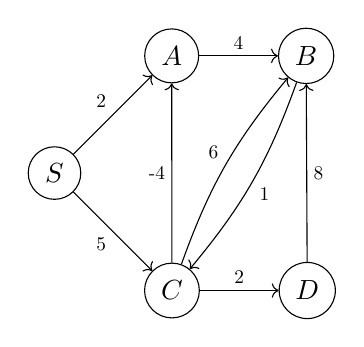
\begin{tikzpicture}[->,baseline,anchor=north]
            \node[draw, circle] (S) {$S$};
            \node[draw, circle, above right=of S] (A) {$A$};
            \node[draw, circle, right=of A] (B) {$B$};
            \node[draw, circle, below right=of S] (C) {$C$};
            \node[draw, circle, right=of C] (D) {$D$};

            \path (S) edge node[weight, above left] {2} (A);
            \path (S) edge node[weight, below left] {5} (C);
            \path (A) edge node[weight, above] {4} (B);
            \path (C) edge node[weight, above] {2} (D);
            \path (C) edge node[weight, left] {-4} (A);
            \path (D) edge node[weight, right] {8} (B);
            \path (B) edge[bend left=10] node[weight, below right] {1} (C);
            \path (C) edge[bend left=10] node[weight, above left] {6} (B);
        \end{tikzpicture}
        %
        \hspace{5em}
        %
        \begin{tabular}{|c||c|c|c|c|c|}
            \hline
              & S & A        & B        & C        & D        \\
            \hline
            0 & 0 & $\infty$ & $\infty$ & $\infty$ & $\infty$ \\
            1 & 0 & 2        & $\infty$ & 5        & $\infty$ \\
            2 & 0 & 1        & 6        & 5        & 7        \\
            3 & 0 & 1        & 5        & 5        & 7        \\
            4 & 0 & 1        & 5        & 5        & 7        \\
            \hline
        \end{tabular}

        Keine Änderungen nach Schritt 3 $\implies$ Fertig!
    \end{center}
\end{example}

\begin{algo}{Floyd-Algorithmus}
    Gegeben: Graph $G = (V, E)$, dessen Bewertungsfunktion die Eigenschaften hat:
    \begin{itemize}
        \item Jede Kante von $v_i$ nach $v_j$ hat nicht-negative Kosten: $C(i, j) \geq 0$
        \item Falls keine Kante zwischen $v_i$ und $v_j$: $C(i, j) = \infty$
        \item Diagonalelemente: $C(i, i) = 0$
    \end{itemize}

    Im Kontrast zum Dijkstra-Algorithmus bestimmt der \emph{Floyd-Algorithmus} für alle geordneten Paare $(v, w)$ den kürzesten Weg von $v$ nach $w$.

    $\abs{V}$ Iterationen:
    \begin{enumerate}
        \item Vergleiche Kosten von
              \begin{itemize}
                  \item direkter Verbindung von Knoten $i$ zu Knoten $j$
                  \item Umweg über Knoten $1$ (also: von $i$ nach $1$ + von $1$ nach $j$)
                  \item Falls Umweg günstiger: alten Weg durch Umweg ersetzen
              \end{itemize}
        \item Umwege über Knoten $2$ betrachten.
        \item[$k$.] Umwege über Knoten $k$ betrachten.
    \end{enumerate}

    Der Floyd-Algorithmus nutzt eine $\abs{V} \times \abs{V}$-Matrix, um die Kosten der günstigsten Wege zu speichern:
    \begin{center}
        $A_k[i][j] :=$ minimale Kosten, um in Schritt $k$ über irgendwelche der Knoten in $V$ vom Knoten $i$ zum Knoten $j$ zu gelangen
    \end{center}

    \begin{itemize}
        \item Initialisierung: $A_0[i][j]= C(i, j)$
        \item $\abs{V}$ Iterationen mit \glqq dynamischer Programmierung\grqq:
              \subitem Iterationsformel zur Aktualisierung von $A[i][j]$:
              $$
                  A_k[i][j] = \min \{ A_{k-1}[i][j] , A_{k-1}[i][k] + A_{k-1}[k][j] \}
              $$
    \end{itemize}

    Der Floyd-Algorithmus ist ein wichtiges Beispiel für dynamische Programmierung.
\end{algo}

\begin{code}{Floyd-Algorithmus}
    \lstinputlisting{floyd.java}
\end{code}

\begin{example}{Floyd-Algorithmus}
    \newcolumntype{g}{>{\columncolor{gray!25}}c}

    $A_0$ (direkter Weg):
    \begin{center}
        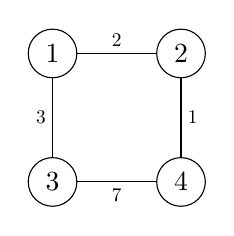
\begin{tikzpicture}[baseline,anchor=north]
            \node[draw, circle] (1) {$1$};
            \node[draw, circle, right=of 1] (2) {$2$};
            \node[draw, circle, below=of 1] (3) {$3$};
            \node[draw, circle, right=of 3] (4) {$4$};

            \path (1) edge node[weight, above] {2} (2);
            \path (1) edge node[weight, left] {3} (3);
            \path (3) edge node[weight, below] {7} (4);
            \path (2) edge node[weight, right] {1} (4);
        \end{tikzpicture}
        %
        \hspace{5em}
        %
        \begin{tabular}[t]{|c|cccc|}
            \hline
              & 1                   & 2                   & 3                   & 4                   \\
            \hline
            1 & \textcolor{gray}{0} & 2                   & 3                   & $\infty$            \\
            2 & 2                   & \textcolor{gray}{0} & $\infty$            & 1                   \\
            3 & 3                   & $\infty$            & \textcolor{gray}{0} & 7                   \\
            4 & $\infty$            & 1                   & 7                   & \textcolor{gray}{0} \\
            \hline
        \end{tabular}
        %
        \hspace{5em}
        %
        \begin{tabular}[t]{|c|cccc|}
            \hline
              & 1                   & 2                   & 3                   & 4 \\
            \hline
            1 & \textcolor{gray}{-} & -                   & -                   & - \\
            2 & -                   & \textcolor{gray}{-} & -                   & - \\
            3 & -                   & -                   & \textcolor{gray}{-} & - \\
            4 & -                   & -                   & -                   & - \\
            \hline
        \end{tabular}
    \end{center}

    $A_1$ (Umweg über 1):
    \begin{center}
        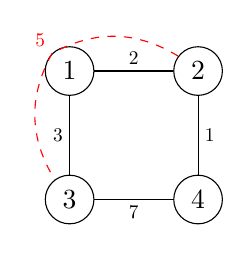
\begin{tikzpicture}[baseline,anchor=north]
            \node[draw, circle] (1) {$1$};
            \node[draw, circle, right=of 1] (2) {$2$};
            \node[draw, circle, below=of 1] (3) {$3$};
            \node[draw, circle, right=of 3] (4) {$4$};

            \path (1) edge node[weight, above] {2} (2);
            \path (1) edge node[weight, left] {3} (3);
            \path (3) edge node[weight, below] {7} (4);
            \path (2) edge node[weight, right] {1} (4);
            %\path (1) edge[blue, bend left=45] node[weight, above, blue] {2} (2);
            %\path (1) edge[blue, bend right=45] node[weight, left, blue] {3} (3);
            \path (2) edge[dashed, red, bend right] node[weight, above left, pos=1] {5} (1.north west);
            \path (1.north west) edge[dashed, red, bend right] (3);
        \end{tikzpicture}
        %
        \hspace{5em}
        %
        \begin{tabular}[t]{|c|gccc|}
            \hline
              & 1                   & 2                   & 3                   & 4                   \\
            \hline
            \rowcolor{gray!25}
            1 & \textcolor{gray}{0} & 2                   & 3                   & $\infty$            \\
            2 & 2                   & \textcolor{gray}{0} & \textcolor{red}{5}  & 1                   \\
            3 & 3                   & \textcolor{red}{5}  & \textcolor{gray}{0} & 7                   \\
            4 & $\infty$            & 1                   & 7                   & \textcolor{gray}{0} \\
            \hline
        \end{tabular}
        %
        \hspace{5em}
        %
        \begin{tabular}[t]{|c|cccc|}
            \hline
              & 1                   & 2                   & 3                   & 4 \\
            \hline
            1 & \textcolor{gray}{-} & -                   & -                   & - \\
            2 & -                   & \textcolor{gray}{-} & 1                   & - \\
            3 & -                   & 1                   & \textcolor{gray}{-} & - \\
            4 & -                   & -                   & -                   & - \\
            \hline
        \end{tabular}
    \end{center}

    $$A_0[2][3] > A_0[3][1] + A_0[1][2] \implies A_1[2][3] = A_0[3][1] + A_0[1][2] = 3 + 2 = 5$$
    $$A_0[3][2] > A_0[2][1] + A_0[1][3] \implies A_1[3][2] = A_0[2][1] + A_0[1][3] = 2 + 3 = 5$$


    $A_2$ (Umweg über 2):
    \begin{center}
        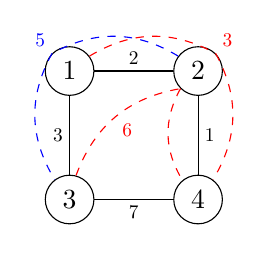
\begin{tikzpicture}[baseline,anchor=north]
            \node[draw, circle] (1) {$1$};
            \node[draw, circle, right=of 1] (2) {$2$};
            \node[draw, circle, below=of 1] (3) {$3$};
            \node[draw, circle, right=of 3] (4) {$4$};

            \path (1) edge node[weight, above] {2} (2);
            \path (1) edge node[weight, left] {3} (3);
            \path (3) edge node[weight, below] {7} (4);
            \path (2) edge node[weight, right] {1} (4);

            % old edge 2-1-3
            \path (2) edge[dashed, blue, bend right] node[weight, above left, pos=1] {5} (1.north west);
            \path (1.north west) edge[dashed, blue, bend right] (3);
            % new edge 1-2-4
            \path (1) edge[dashed, red, bend left] node[weight, above right, pos=1] {3} (2.north east);
            \path (2.north east) edge[dashed, red, bend left] (4);
            % old edge 3-2-4
            \path (3) edge[dashed, red, bend left] node[weight, below right, pos=0.5] {6} (2.south west);
            \path (2.south west) edge[dashed, red, bend right] (4);
        \end{tikzpicture}
        %
        \hspace{5em}
        %
        \begin{tabular}[t]{|c|cgcc|}
            \hline
              & 1                   & 2                   & 3                   & 4                   \\
            \hline
            1 & \textcolor{gray}{0} & 2                   & 3                   & \textcolor{red}{3}  \\
            \rowcolor{gray!25}
            2 & 2                   & \textcolor{gray}{0} & 5                   & 1                   \\
            3 & 3                   & 5                   & \textcolor{gray}{0} & \textcolor{red}{6}  \\
            4 & \textcolor{red}{3}  & 1                   & \textcolor{red}{6}  & \textcolor{gray}{0} \\
            \hline
        \end{tabular}
        %
        \hspace{5em}
        %
        \begin{tabular}[t]{|c|cccc|}
            \hline
              & 1                   & 2                   & 3                   & 4 \\
            \hline
            1 & \textcolor{gray}{-} & -                   & -                   & 2 \\
            2 & -                   & \textcolor{gray}{-} & 1                   & - \\
            3 & -                   & 1                   & \textcolor{gray}{-} & 2 \\
            4 & 2                   & -                   & 2                   & - \\
            \hline
        \end{tabular}
    \end{center}

    $$A_1[1][4] > A_1[1][2] + A_1[2][4] \implies A_2[2][3] = A_1[1][2] + A_1[2][4] = 2 + 1 = 3$$
    $$A_1[4][1] > A_1[4][2] + A_1[2][1] \implies A_2[3][2] = A_1[4][2] + A_1[2][1] = 1 + 2 = 3$$
    $$A_1[3][4] > A_1[3][2] + A_1[2][4] \implies A_2[3][4] = A_1[3][2] + A_1[2][4] = 5 + 1 = 6$$
    $$A_1[4][3] > A_1[4][2] + A_1[2][3] \implies A_2[4][3] = A_1[4][2] + A_1[2][3] = 1 + 5 = 6$$

    $A_3$ (Umweg über 3):
    \begin{center}
        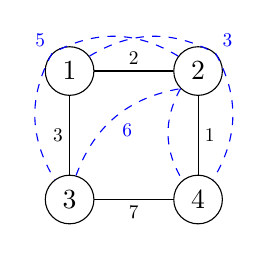
\begin{tikzpicture}[baseline,anchor=north]
            \node[draw, circle] (1) {$1$};
            \node[draw, circle, right=of 1] (2) {$2$};
            \node[draw, circle, below=of 1] (3) {$3$};
            \node[draw, circle, right=of 3] (4) {$4$};

            \path (1) edge node[weight, above] {2} (2);
            \path (1) edge node[weight, left] {3} (3);
            \path (3) edge node[weight, below] {7} (4);
            \path (2) edge node[weight, right] {1} (4);

            % old edge 2-1-3
            \path (2) edge[dashed, blue, bend right] node[weight, above left, pos=1] {5} (1.north west);
            \path (1.north west) edge[dashed, blue, bend right] (3);
            % old edge 1-2-4
            \path (1) edge[dashed, blue, bend left] node[weight, above right, pos=1] {3} (2.north east);
            \path (2.north east) edge[dashed, blue, bend left] (4);
            % old edge 3-2-4
            \path (3) edge[dashed, blue, bend left] node[weight, below right, pos=0.5] {6} (2.south west);
            \path (2.south west) edge[dashed, blue, bend right] (4);
        \end{tikzpicture}
        %
        \hspace{5em}
        %
        \begin{tabular}[t]{|c|ccgc|}
            \hline
              & 1                   & 2                   & 3                   & 4                   \\
            \hline
            1 & \textcolor{gray}{0} & 2                   & 3                   & 3                   \\
            2 & 2                   & \textcolor{gray}{0} & 5                   & 1                   \\
            \rowcolor{gray!25}
            3 & 3                   & 5                   & \textcolor{gray}{0} & 6                   \\
            4 & 3                   & 1                   & 6                   & \textcolor{gray}{0} \\
            \hline
        \end{tabular}
        %
        \hspace{5em}
        %
        \begin{tabular}[t]{|c|cccc|}
            \hline
              & 1                   & 2                   & 3                   & 4 \\
            \hline
            1 & \textcolor{gray}{-} & -                   & -                   & 2 \\
            2 & -                   & \textcolor{gray}{-} & 1                   & - \\
            3 & -                   & 1                   & \textcolor{gray}{-} & 2 \\
            4 & 2                   & -                   & 2                   & - \\
            \hline
        \end{tabular}
    \end{center}

    $A_4$ (Umweg über 4):
    \begin{center}
        \begin{tikzpicture}[baseline,anchor=north]
            \node[draw, circle] (1) {$1$};
            \node[draw, circle, right=of 1] (2) {$2$};
            \node[draw, circle, below=of 1] (3) {$3$};
            \node[draw, circle, right=of 3] (4) {$4$};

            \path (1) edge node[weight, above] {2} (2);
            \path (1) edge node[weight, left] {3} (3);
            \path (3) edge node[weight, below] {7} (4);
            \path (2) edge node[weight, right] {1} (4);

            % old edge 2-1-3
            \path (2) edge[dashed, blue, bend right] node[weight, above left, pos=1] {5} (1.north west);
            \path (1.north west) edge[dashed, blue, bend right] (3);
            % old edge 1-2-4
            \path (1) edge[dashed, blue, bend left] node[weight, above right, pos=1] {3} (2.north east);
            \path (2.north east) edge[dashed, blue, bend left] (4);
            % old edge 3-2-4
            \path (3) edge[dashed, blue, bend left] node[weight, below right, pos=0.5] {6} (2.south west);
            \path (2.south west) edge[dashed, blue, bend right] (4);
        \end{tikzpicture}
        %
        \hspace{5em}
        %
        \begin{tabular}[t]{|c|cccg|}
            \hline
              & 1                   & 2                   & 3                   & 4                   \\
            \hline
            1 & \textcolor{gray}{0} & 2                   & 3                   & 3                   \\
            2 & 2                   & \textcolor{gray}{0} & 5                   & 1                   \\
            3 & 3                   & 5                   & \textcolor{gray}{0} & 6                   \\
            \rowcolor{gray!25}
            4 & 3                   & 1                   & 6                   & \textcolor{gray}{0} \\
            \hline
        \end{tabular}
        %
        \hspace{5em}
        %
        \begin{tabular}[t]{|c|cccc|}
            \hline
              & 1                   & 2                   & 3                   & 4 \\
            \hline
            1 & \textcolor{gray}{-} & -                   & -                   & 2 \\
            2 & -                   & \textcolor{gray}{-} & 1                   & - \\
            3 & -                   & 1                   & \textcolor{gray}{-} & 2 \\
            4 & 2                   & -                   & 2                   & - \\
            \hline
        \end{tabular}
    \end{center}
\end{example}

\begin{algo}{Warshall-Algorithmus}
    Gegeben: Graph $G = (V, E)$, egal ob gerichtet oder nicht.

    Aufgabenstellung: Prüfe für alle geordneten Paare $(v_i, v_j)$, ob ein Weg von $v_i$ nach $v_j$ existiert.

    Ziel: Berechne Adjazenzmatrix $A$ zu \emph{transitivem Abschluss} von $G$:
    \begin{center}
        $A[i][j] = $ \texttt{true} $\iff$ es existiert ein nicht-trivialer Weg (Länge $>0$) von $v_i$ nach $v_j$
    \end{center}

    Iterationsformel zur Aktualisierung von $A[i][j]$:
    $$
        A_k[i][j] = A_{k-1}[i][j] \lor (A_{k-1}[i][k] \land A_{k-1}[k][j])
    $$

    Der Algorithmus funktioniert also analog zum Floyd-Algorithmus.
\end{algo}

\begin{code}{Warshall-Algorithmus}
    \lstinputlisting{warshall.java}
\end{code}

\section{Formale Sprachen}
% Textsuche
\subsection{Textsuche}

\begin{bonus}{Textsucheverfahren}
    \begin{itemize}
        \item Naiver, grober, oder brute-force-Algorithmus $\in \bigo(n \cdot m)$
              \begin{itemize}
                  \item für kleine Texte am schnellsten
              \end{itemize}
        \item Knuth-Morris-Pratt, Rabin-Karp $\in \Theta(n + m)$
        \item Boyer-Moore, (Boyer-Moore)-Sunday, (Boyer-Moore)-Horsepool $\in \bigo(n + m)$
              \begin{itemize}
                  \item für große Texte am schnellsten
              \end{itemize}
    \end{itemize}
\end{bonus}

\begin{algo}{Naive Textsuche}
    Bei der \emph{naiven Textsuche} wird an allen Positionen $i$ des Textes nach dem Muster geprüft.

    Die möglichen Positionen reichen von $i=0$ (Muster linksbündig mit dem Text) bis $i = n-m$ (Muster rechtsbündig mit dem Text).

    Das Muster wird an der jeweiligen Position zeichenweise von links nach rechts mit dem Text verglichen.

    Bei einem \emph{Mismatch} oder bei vollständiger Übereinstimmung (\emph{Match}) wird das Muster um eine Position weitergeschoben und an dieser Position verglichen.
\end{algo}

\begin{example}{Naive Textsuche}
    \textbf{Aufgabe:} Finde das Muster \texttt{SINN} im Text \texttt{DASISTSINNLOSERTEXT} mithilfe naiver Textsuche.

    \centering

    \vspace{1em}

    \begin{tikzpicture}[
        start chain,
        node distance = 0pt,
        TextBlock/.style={draw, minimum width=2em, minimum height=2em, outer sep=0pt, on chain},
        ]
        { start chain = going right
        %\node [TextBlock, fill=red!50, label=$0$] (0) {};
        \node [TextBlock] (00) {D};
        \node [TextBlock] (01) {A};
        \node [TextBlock] (02) {S};
        \node [TextBlock] (03) {I};
        \node [TextBlock] (04) {S};
        \node [TextBlock] (05) {T};
        \node [TextBlock] (06) {S};
        \node [TextBlock] (07) {I};
        \node [TextBlock] (08) {N};
        \node [TextBlock] (09) {N};
        \node [TextBlock] (10) {L};
        \node [TextBlock] (11) {O};
        \node [TextBlock] (12) {S};
        \node [TextBlock] (13) {E};
        \node [TextBlock] (14) {R};
        \node [TextBlock] (15) {T};
        \node [TextBlock] (16) {E};
        \node [TextBlock] (17) {X};
        \node [TextBlock] (18) {T};


        { [continue chain = going right]
        \chainin (00);

        \node[TextBlock, xshift=-2em, yshift=2em, index] () {\tiny 0};
        \node [TextBlock, index] () {\tiny 1};
        \node [TextBlock, index] () {\tiny 2};
        \node [TextBlock, index] () {\tiny 3};
        \node [TextBlock, index] () {\tiny 4};
        \node [TextBlock, index] () {\tiny 5};
        \node [TextBlock, index] () {\tiny 6};
        \node [TextBlock, index] () {\tiny 7};
        \node [TextBlock, index] () {\tiny 8};
        \node [TextBlock, index] () {\tiny 9};
        \node [TextBlock, index] () {\tiny 10};
        \node [TextBlock, index] () {\tiny 11};
        \node [TextBlock, index] () {\tiny 12};
        \node [TextBlock, index] () {\tiny 13};
        \node [TextBlock, index] () {\tiny 14};
        \node [TextBlock, index] () {\tiny 15};
        \node [TextBlock, index] () {\tiny 16};
        \node [TextBlock, index] () {\tiny 17};
        \node [TextBlock, index] () {\tiny 18};
        }

        { [continue chain = going right]
        \chainin (00);
        \node[TextBlock, xshift=-2em, yshift=-2em, fill=red!50] (1_0) {S};
        \node[TextBlock] (1_1) {I};
        \node[TextBlock] (1_2) {N};
        \node[TextBlock] (1_3) {N};
        %
        \node[on chain, xshift=2em] (1_info) {\texttt{i=0; j=0} $\implies$ Mismatch!};
        }

        { [continue chain = going right]
        \chainin (01);
        \node[TextBlock, xshift=-2em, yshift=-4em, fill=red!50] (1_0) {S};
        \node[TextBlock] (2_1) {I};
        \node[TextBlock] (2_2) {N};
        \node[TextBlock] (2_3) {N};
        %
        \node[on chain, xshift=2em] (1_info) {\texttt{i=1; j=0} $\implies$ Mismatch!};
        }

        { [continue chain = going right]
        \chainin (02);
        \node[TextBlock, xshift=-2em, yshift=-6em, fill=teal!50] (1_0) {S};
        \node[TextBlock, fill=teal!50] (3_1) {I};
        \node[TextBlock, fill=red!50] (3_2) {N};
        \node[TextBlock] (3_3) {N};
        %
        \node[on chain, xshift=2em] (1_info) {\texttt{i=2; j=2} $\implies$ Mismatch!};
        }

        { [continue chain = going right]
        \chainin (03);
        \node[TextBlock, xshift=-2em, yshift=-8em, fill=red!50] (1_0) {S};
        \node[TextBlock] (4_1) {I};
        \node[TextBlock] (4_2) {N};
        \node[TextBlock] (4_3) {N};
        %
        \node[on chain, xshift=2em] (1_info) {\texttt{i=3; j=0} $\implies$ Mismatch!};
        }

        { [continue chain = going right]
        \chainin (04);
        \node[TextBlock, xshift=-2em, yshift=-10em, fill=teal!50] (1_0) {S};
        \node[TextBlock, fill=red!50] (5_1) {I};
        \node[TextBlock] (5_2) {N};
        \node[TextBlock] (5_3) {N};
        %
        \node[on chain, xshift=2em] (1_info) {\texttt{i=4; j=1} $\implies$ Mismatch!};
        }

        { [continue chain = going right]
        \chainin (05);
        \node[TextBlock, xshift=-2em, yshift=-12em, fill=red!50] (1_0) {S};
        \node[TextBlock] (5_1) {I};
        \node[TextBlock] (5_2) {N};
        \node[TextBlock] (5_3) {N};
        %
        \node[on chain, xshift=2em] (1_info) {\texttt{i=5; j=0} $\implies$ Mismatch!};
        }

        { [continue chain = going right]
        \chainin (06);
        \node[TextBlock, xshift=-2em, yshift=-14em, fill=teal!50] (1_0) {S};
        \node[TextBlock, fill=teal!50] (5_1) {I};
        \node[TextBlock, fill=teal!50] (5_2) {N};
        \node[TextBlock, fill=teal!50] (5_3) {N};
        %
        \node[on chain, xshift=2em] (1_info) {\textcolor{teal}{\texttt{i=6; j=4} $\implies$ Match!}};
        }
        }
    \end{tikzpicture}
\end{example}

\begin{algo}{Knuth-Morris-Pratt-Algorithmus}
    Der \emph{Knuth-Morris-Pratt-Algorithmus} baut auf der naiven Textsuche auf.

    Der Unterschied liegt darin, dass bei einem Mismatch das Muster nicht nur um eine Position verschoben werden kann, sondern um mehrere gleichzeitig.
    Dabei gilt:
    \begin{itemize}
        \item \textbf{Fall 1:} Wenn die letzten überprüften Buchstaben gleich dem Anfang des Patterns sind, verschiebt man das Muster entsprechend und macht beim anschließenden Zeichen weiter.
        \item \textbf{Fall 2:} Wenn die letzten überprüften Buchstaben nicht gleich dem Anfang des Musters sind, verschiebt man das Muster so, dass das erste Zeichen auf dem Mismatch zu liegen kommt.
    \end{itemize}
\end{algo}

\begin{example}{Knuth-Morris-Pratt-Algorithmus}
    \textbf{Aufgabe:} Finde das Muster \texttt{UNGLEICHUNGEN} im Text \texttt{UNGLEICHUNGSTEIL...} mithilfe des Knuth-Morris-Pratt-Algorithmus.

    \vspace{1em}

    \begin{center}
        \begin{tikzpicture}[
            start chain,
            node distance = 0pt,
            TextBlock/.style={draw, minimum width=2em, minimum height=2em, outer sep=0pt, on chain},
            ]
            { start chain = going right
            \node [TextBlock] (00) {U};
            \node [TextBlock] (01) {N};
            \node [TextBlock] (02) {G};
            \node [TextBlock] (03) {L};
            \node [TextBlock] (04) {E};
            \node [TextBlock] (05) {I};
            \node [TextBlock] (06) {C};
            \node [TextBlock] (07) {H};
            \node [TextBlock] (08) {U};
            \node [TextBlock] (09) {N};
            \node [TextBlock] (10) {G};
            \node [TextBlock] (11) {S};
            \node [TextBlock] (12) {T};
            \node [TextBlock] (13) {E};
            \node [TextBlock] (14) {I};
            \node [TextBlock] (15) {L};
            \node [TextBlock] (16) {$\ldots$};

            { [continue chain = going right]
            \chainin (00);

            \node[TextBlock, xshift=-2em, yshift=2em, index] () {\tiny 0};
            \node [TextBlock, index] () {\tiny 1};
            \node [TextBlock, index] () {\tiny 2};
            \node [TextBlock, index] () {\tiny 3};
            \node [TextBlock, index] () {\tiny 4};
            \node [TextBlock, index] () {\tiny 5};
            \node [TextBlock, index] () {\tiny 6};
            \node [TextBlock, index] () {\tiny 7};
            \node [TextBlock, index] () {\tiny 8};
            \node [TextBlock, index] () {\tiny 9};
            \node [TextBlock, index] () {\tiny 10};
            \node [TextBlock, index] () {\tiny 11};
            \node [TextBlock, index] () {\tiny 12};
            \node [TextBlock, index] () {\tiny 13};
            \node [TextBlock, index] () {\tiny 14};
            \node [TextBlock, index] () {\tiny 15};
            \node [TextBlock, index] () {\tiny 16};
            }


            { [continue chain = going right]
            \chainin (00);
            \node[TextBlock, xshift=-2em, yshift=-2em, fill=teal!50] (1_00)  {U};
            \node [TextBlock, fill=teal!50] (1_01) {N};
            \node [TextBlock, fill=teal!50] (1_02) {G};
            \node [TextBlock, fill=teal!50] (1_03) {L};
            \node [TextBlock, fill=teal!50] (1_04) {E};
            \node [TextBlock, fill=teal!50] (1_05) {I};
            \node [TextBlock, fill=teal!50] (1_06) {C};
            \node [TextBlock, fill=teal!50] (1_07) {H};
            \node [TextBlock, fill=teal!50] (1_08) {U};
            \node [TextBlock, fill=teal!50] (1_09) {N};
            \node [TextBlock, fill=teal!50] (1_10) {G};
            \node [TextBlock, fill=red!50] (1_11) {E};
            \node [TextBlock] (1_12) {N};
            %
            \node[on chain, xshift=2em] (1_info) {$\implies$ Fall 1};
            }

            { [continue chain = going right]
            \chainin (08);
            \node[TextBlock, xshift=-2em, yshift=-4em, fill=teal!50] (2_00)  {U};
            \node [TextBlock, fill=teal!50] (2_01) {N};
            \node [TextBlock, fill=teal!50] (2_02) {G};
            \node [TextBlock, fill=red!50] (2_03) {L};
            \node [TextBlock] (2_04) {E};
            \node [TextBlock] (2_05) {I};
            \node [TextBlock] (2_06) {C};
            \node [TextBlock] (2_07) {H};
            \node [TextBlock] (2_08) {$\ldots$};
            }

            { [continue chain = going below]
            \chainin (2_00);
            \node [on chain, minimum width=2em, minimum height=2em] (usw) {usw.};
            }
            }
            \node [draw, dashed, fit={(00) (01) (02) (1_00) (1_01) (1_02)}] {};
            \node [draw, dashed, fit={(08) (09) (10) (1_08) (1_09) (1_10)}] {};
        \end{tikzpicture}
    \end{center}

    \textbf{Aufgabe:} Finde das Muster \texttt{UNGLEICHER} im Text \texttt{UNGLEICHUNGSTEIL...} mithilfe des Knuth-Morris-Pratt-Algorithmus.

    \vspace{1em}

    \begin{center}
        \begin{tikzpicture}[
            start chain,
            node distance = 0pt,
            TextBlock/.style={draw, minimum width=2em, minimum height=2em, outer sep=0pt, on chain},
            ]
            { start chain = going right
            \node [TextBlock] (00) {U};
            \node [TextBlock] (01) {N};
            \node [TextBlock] (02) {G};
            \node [TextBlock] (03) {L};
            \node [TextBlock] (04) {E};
            \node [TextBlock] (05) {I};
            \node [TextBlock] (06) {C};
            \node [TextBlock] (07) {H};
            \node [TextBlock] (08) {U};
            \node [TextBlock] (09) {N};
            \node [TextBlock] (10) {G};
            \node [TextBlock] (11) {S};
            \node [TextBlock] (12) {T};
            \node [TextBlock] (13) {E};
            \node [TextBlock] (14) {I};
            \node [TextBlock] (15) {L};
            \node [TextBlock] (16) {$\ldots$};

            { [continue chain = going right]
            \chainin (00);

            \node[TextBlock, xshift=-2em, yshift=2em, index] () {\tiny 0};
            \node [TextBlock, index] () {\tiny 1};
            \node [TextBlock, index] () {\tiny 2};
            \node [TextBlock, index] () {\tiny 3};
            \node [TextBlock, index] () {\tiny 4};
            \node [TextBlock, index] () {\tiny 5};
            \node [TextBlock, index] () {\tiny 6};
            \node [TextBlock, index] () {\tiny 7};
            \node [TextBlock, index] () {\tiny 8};
            \node [TextBlock, index] () {\tiny 9};
            \node [TextBlock, index] () {\tiny 10};
            \node [TextBlock, index] () {\tiny 11};
            \node [TextBlock, index] () {\tiny 12};
            \node [TextBlock, index] () {\tiny 13};
            \node [TextBlock, index] () {\tiny 14};
            \node [TextBlock, index] () {\tiny 15};
            \node [TextBlock, index] () {\tiny 16};
            }

            { [continue chain = going right]
            \chainin (00);
            \node[TextBlock, xshift=-2em, yshift=-2em, fill=teal!50] (1_00)  {U};
            \node [TextBlock, fill=teal!50] (1_01) {N};
            \node [TextBlock, fill=teal!50] (1_02) {G};
            \node [TextBlock, fill=teal!50] (1_03) {L};
            \node [TextBlock, fill=teal!50] (1_04) {E};
            \node [TextBlock, fill=teal!50] (1_05) {I};
            \node [TextBlock, fill=teal!50] (1_06) {C};
            \node [TextBlock, fill=teal!50] (1_07) {H};
            \node [TextBlock, fill=red!50] (1_08) {E};
            \node [TextBlock] (1_09) {R};
            %
            \node[on chain, xshift=2em] (1_info) {$\implies$ Fall 2};
            }

            { [continue chain = going right]
            \chainin (08);
            \node[TextBlock, xshift=-2em, yshift=-4em, fill=teal!50] (2_00)  {U};
            \node [TextBlock, fill=teal!50] (2_01) {N};
            \node [TextBlock, fill=teal!50] (2_02) {G};
            \node [TextBlock, fill=red!50] (2_03) {L};
            \node [TextBlock] (2_04) {E};
            \node [TextBlock] (2_05) {I};
            \node [TextBlock] (2_06) {C};
            \node [TextBlock] (2_07) {H};
            \node [TextBlock] (2_08) {$\ldots$};
            }

            { [continue chain = going below]
            \chainin (2_00);
            \node [on chain, minimum width=2em, minimum height=2em] (usw) {usw.};
            }
            }
        \end{tikzpicture}
    \end{center}
\end{example}

\begin{algo}{Boyer-Moore-Sunday-Algorithmus}
    Beim \emph{Boyer-Moore-Sunday-Algorithmus} wird nach einem Mismatch das Zeichen betrachtet, das hinter dem Muster liegt.

    Dabei kann das Muster so weit nach vorne geschoben werden, bis ein Buchstabe des Musters mit diesem Buchstaben übereinstimmt.\footnote{Taucht der Buchstabe mehrfach im Wort auf, wird um die geringste Distanz nach vorne geschoben - also an den Buchstaben, der im Muster am weitesten hinten liegt.}

    Kommt der folgende Buchstabe im Muster nicht vor, wird das Muster über den Buchstaben hinweggeschoben, da alle Positionen vorher sowieso zwecklos sind.
\end{algo}

\begin{example}{Boyer-Moore-Sunday-Algorithmus}
    \textbf{Aufgabe:} Finde das Muster \texttt{ACBABCBA} im Text \texttt{AABBACCBACDACBABCBA} mithilfe des Boyer-Moore-Sunday-Algorithmus.

    \centering

    \vspace{1em}

    \begin{tikzpicture}[
        start chain,
        node distance = 0pt,
        TextBlock/.style={draw, minimum width=2em, minimum height=2em, outer sep=0pt, on chain},
        hit/.style={fill=teal!50},
        miss/.style={fill=red!50},
        next/.style={fill=blue!25},
        ]
        { start chain = going right
        %\node [TextBlock, fill=red!50, label=$0$] (0) {};
        \node [TextBlock] (00) {A};
        \node [TextBlock] (01) {A};
        \node [TextBlock] (02) {B};
        \node [TextBlock] (03) {B};
        \node [TextBlock] (04) {A};
        \node [TextBlock] (05) {C};
        \node [TextBlock] (06) {C};
        \node [TextBlock] (07) {B};
        \node [TextBlock] (08) {A};
        \node [TextBlock] (09) {C};
        \node [TextBlock] (10) {D};
        \node [TextBlock] (11) {A};
        \node [TextBlock] (12) {C};
        \node [TextBlock] (13) {B};
        \node [TextBlock] (14) {A};
        \node [TextBlock] (15) {B};
        \node [TextBlock] (16) {C};
        \node [TextBlock] (17) {B};
        \node [TextBlock] (18) {A};

        { [continue chain = going right]
        \chainin (00);

        \node[TextBlock, xshift=-2em, yshift=2em, index] () {\tiny 0};
        \node [TextBlock, index] () {\tiny 1};
        \node [TextBlock, index] () {\tiny 2};
        \node [TextBlock, index] () {\tiny 3};
        \node [TextBlock, index] () {\tiny 4};
        \node [TextBlock, index] () {\tiny 5};
        \node [TextBlock, index] () {\tiny 6};
        \node [TextBlock, index] () {\tiny 7};
        \node [TextBlock, index] () {\tiny 8};
        \node [TextBlock, index] () {\tiny 9};
        \node [TextBlock, index] () {\tiny 10};
        \node [TextBlock, index] () {\tiny 11};
        \node [TextBlock, index] () {\tiny 12};
        \node [TextBlock, index] () {\tiny 13};
        \node [TextBlock, index] () {\tiny 14};
        \node [TextBlock, index] () {\tiny 15};
        \node [TextBlock, index] () {\tiny 16};
        \node [TextBlock, index] () {\tiny 17};
        \node [TextBlock, index] () {\tiny 18};
        }

        { [continue chain = going right]
        \chainin (00);

        \node[TextBlock, xshift=-2em, yshift=-2em, hit] (1_00) {A};
        \node [TextBlock, miss] (1_01) {C};
        \node [TextBlock] (1_02) {B};
        \node [TextBlock] (1_03) {A};
        \node [TextBlock] (1_04) {B};
        \node [TextBlock] (1_05) {C};
        \node [TextBlock] (1_06) {B};
        \node [TextBlock] (1_07) {A};
        }

        { [continue chain = going right]
        \chainin (01);

        \node[TextBlock, xshift=-2em, yshift=-4em, hit] (2_00) {A};
        \node [TextBlock, miss] (2_01) {C};
        \node [TextBlock] (2_02) {B};
        \node [TextBlock] (2_03) {A};
        \node [TextBlock] (2_04) {B};
        \node [TextBlock] (2_05) {C};
        \node [TextBlock] (2_06) {B};
        \node [TextBlock, next] (2_07) {A};
        }

        { [continue chain = going right]
        \chainin (04);

        \node[TextBlock, xshift=-2em, yshift=-6em, hit] (3_00) {A};
        \node [TextBlock, hit] (3_01) {C};
        \node [TextBlock, miss] (3_02) {B};
        \node [TextBlock] (3_03) {A};
        \node [TextBlock] (3_04) {B};
        \node [TextBlock, next] (3_05) {C};
        \node [TextBlock] (3_06) {B};
        \node [TextBlock] (3_07) {A};
        }

        { [continue chain = going right]
        \chainin (07);

        \node[TextBlock, xshift=-2em, yshift=-8em, miss] (4_00) {A};
        \node [TextBlock] (4_01) {C};
        \node [TextBlock] (4_02) {B};
        \node [TextBlock] (4_03) {A};
        \node [TextBlock] (4_04) {B};
        \node [TextBlock, next] (4_05) {C};
        \node [TextBlock] (4_06) {B};
        \node [TextBlock] (4_07) {A};
        }

        { [continue chain = going right]
        \chainin (09);

        \node[TextBlock, xshift=-2em, yshift=-10em, miss] (5_00) {A};
        \node [TextBlock] (5_01) {C};
        \node [TextBlock] (5_02) {B};
        \node [TextBlock] (5_03) {A};
        \node [TextBlock] (5_04) {B};
        \node [TextBlock] (5_05) {C};
        \node [TextBlock, next] (5_06) {B};
        \node [TextBlock] (5_07) {A};
        }

        { [continue chain = going right]
        \chainin (11);

        \node[TextBlock, xshift=-2em, yshift=-12em, hit] (6_00) {A};
        \node [TextBlock, hit] (6_01) {C};
        \node [TextBlock, hit] (6_02) {B};
        \node [TextBlock, hit] (6_03) {A};
        \node [TextBlock, hit] (6_04) {B};
        \node [TextBlock, hit] (6_05) {C};
        \node [TextBlock, next] (6_06) {B};
        \node [TextBlock, hit] (6_07) {A};
        }
        }
        \draw[->] (08) to (2_07);
        \draw[->] (09) to (3_05);
        \draw[->] (12) to (4_05);
        \draw[->] (15) to (5_06);
        \draw[->] (17) to (6_06);
    \end{tikzpicture}
\end{example}

\begin{defi}{\texttt{last}-Tabelle}
    Die \texttt{last}\emph{-Tabelle} enthält zu jedem Zeichen des Zeichensatzes die Position des letzten Vorkommens im Muster (oder $-1$, falls es nicht vorkommt).

    Die Implementierung erfolgt z.B. als Array indiziert mit (Unicode-)Zeichensatz:
    \begin{itemize}
        \item \texttt{A} auf Index $65$
        \item \texttt{B} auf Index $66$
        \item $\ldots$
        \item \texttt{a} auf Index $97$
        \item \texttt{b} auf Index $98$
        \item $\ldots$
    \end{itemize}

    Dabei gilt:
    \begin{itemize}
        \item Alte Position des Patterns: \texttt{i} (das Pattern reicht bis \texttt{i + m - 1})
        \item Verschiebedistanz: \texttt{v = m - last[text[i+m]]}
        \item Neue Position des Patterns: \texttt{i + v} (das Pattern reicht bis \texttt{i + v +  m - 1})
    \end{itemize}
\end{defi}

\begin{example}{Boyer-Moore-Sunday-Algorithmus mit \texttt{last}-Tabelle}
    \textbf{Aufgabe:} Finde das Muster \texttt{BANANAS} im Text \texttt{ORANGES, ANANANAS AND BANANANAS} mithilfe des Boyer-Moore-Sunday-Algorithmus und einer \texttt{last}-Tabelle.

    \centering

    \vspace{1em}

    \begin{tabular}{|l||cccc|c|}
        \hline
        Pattern            & B & A & N & S & sonst \\
        \hline
        \texttt{last}-Wert & 0 & 5 & 4 & 6 & -1    \\
        \hline
    \end{tabular}

    \vspace{1em}

    \begin{tikzpicture}[
        start chain,
        node distance = 0pt,
        TextBlock/.style={draw, minimum width=1.5em, minimum height=1.5em, outer sep=0pt, on chain},
        hit/.style={fill=teal!50},
        miss/.style={fill=red!50},
        next/.style={fill=blue!25},
        ]
        { start chain = going right
        %\node [TextBlock, fill=red!50, label=$0$] (0) {};
        \node [TextBlock] (00) {O};
        \node [TextBlock] (01) {R};
        \node [TextBlock] (02) {A};
        \node [TextBlock] (03) {N};
        \node [TextBlock] (04) {G};
        \node [TextBlock] (05) {E};
        \node [TextBlock] (06) {S};
        \node [TextBlock] (07) {,};
        \node [TextBlock] (08) {};
        \node [TextBlock] (09) {A};
        \node [TextBlock] (10) {N};
        \node [TextBlock] (11) {A};
        \node [TextBlock] (12) {N};
        \node [TextBlock] (13) {A};
        \node [TextBlock] (14) {S};
        \node [TextBlock] (15) {};
        \node [TextBlock] (16) {A};
        \node [TextBlock] (17) {N};
        \node [TextBlock] (18) {D};
        \node [TextBlock] (19) {};
        \node [TextBlock] (20) {B};
        \node [TextBlock] (21) {A};
        \node [TextBlock] (22) {N};
        \node [TextBlock] (23) {A};
        \node [TextBlock] (24) {N};
        \node [TextBlock] (25) {A};
        \node [TextBlock] (26) {S};

        { [continue chain = going right]
        \chainin (00);

        \node[TextBlock, xshift=-1.5em, yshift=1.5em, index small] () {\tiny 0};
        \node [TextBlock, index small] () {\tiny 1};
        \node [TextBlock, index small] () {\tiny 2};
        \node [TextBlock, index small] () {\tiny 3};
        \node [TextBlock, index small] () {\tiny 4};
        \node [TextBlock, index small] () {\tiny 5};
        \node [TextBlock, index small] () {\tiny 6};
        \node [TextBlock, index small] () {\tiny 7};
        \node [TextBlock, index small] () {\tiny 8};
        \node [TextBlock, index small] () {\tiny 9};
        \node [TextBlock, index small] () {\tiny 10};
        \node [TextBlock, index small] () {\tiny 11};
        \node [TextBlock, index small] () {\tiny 12};
        \node [TextBlock, index small] () {\tiny 13};
        \node [TextBlock, index small] () {\tiny 14};
        \node [TextBlock, index small] () {\tiny 15};
        \node [TextBlock, index small] () {\tiny 16};
        \node [TextBlock, index small] () {\tiny 17};
        \node [TextBlock, index small] () {\tiny 18};
        \node [TextBlock, index small] () {\tiny 19};
        \node [TextBlock, index small] () {\tiny 20};
        \node [TextBlock, index small] () {\tiny 21};
        \node [TextBlock, index small] () {\tiny 22};
        \node [TextBlock, index small] () {\tiny 23};
        \node [TextBlock, index small] () {\tiny 24};
        \node [TextBlock, index small] () {\tiny 25};
        \node [TextBlock, index small] () {\tiny 26};
        }

        { [continue chain = going right]
        \chainin (00);

        \node[TextBlock, xshift=-1.5em, yshift=-1.5em, miss] (1_00) {B};
        \node [TextBlock] (1_01) {A};
        \node [TextBlock] (1_02) {N};
        \node [TextBlock] (1_03) {A};
        \node [TextBlock] (1_04) {N};
        \node [TextBlock] (1_05) {A};
        \node [TextBlock] (1_06) {S};
        }

        { [continue chain = going right]
        \chainin (08);

        \node [TextBlock, xshift=-3em, yshift=-3em, dashed, blue] (2_left) {};
        \node [TextBlock, miss] (2_00) {B};
        \node [TextBlock] (2_01) {A};
        \node [TextBlock] (2_02) {N};
        \node [TextBlock] (2_03) {A};
        \node [TextBlock] (2_04) {N};
        \node [TextBlock] (2_05) {A};
        \node [TextBlock] (2_06) {S};
        }

        { [continue chain = going right]
        \chainin (16);

        \node [TextBlock, xshift=-3em, yshift=-4.5em, dashed, blue] (3_left) {};
        \node [TextBlock, miss] (3_00) {B};
        \node [TextBlock] (3_01) {A};
        \node [TextBlock] (3_02) {N};
        \node [TextBlock] (3_03) {A};
        \node [TextBlock] (3_04) {N};
        \node [TextBlock] (3_05) {A};
        \node [TextBlock] (3_06) {S};
        }

        { [continue chain = going right]
        \chainin (18);

        \node [TextBlock, xshift=-1.5em, yshift=-6em, miss] (4_00) {B};
        \node [TextBlock] (4_01) {A};
        \node [TextBlock] (4_02) {N};
        \node [TextBlock] (4_03) {A};
        \node [TextBlock] (4_04) {N};
        \node [TextBlock, next] (4_05) {A};
        \node [TextBlock] (4_06) {S};
        }

        { [continue chain = going right]
        \chainin (20);

        \node [TextBlock, xshift=-1.5em, yshift=-7.5em, hit] (5_00) {B};
        \node [TextBlock, hit] (5_01) {A};
        \node [TextBlock, hit] (5_02) {N};
        \node [TextBlock, hit] (5_03) {A};
        \node [TextBlock, hit] (5_04) {N};
        \node [TextBlock, next] (5_05) {A};
        \node [TextBlock, hit] (5_06) {S};
        }
        }
        \draw[->] (07) to node [midway, right] () {\small \color{blue} \texttt{v = 8}} (2_left);
        \draw[->] (15) to node [midway, right] () {\small \color{blue} \texttt{v = 8}} (3_left);
        \draw[->] (23) to node [midway, right] () {\small \color{blue} \texttt{v = 2}} (4_05);
        \draw[->] (25) to node [midway, right] () {\small \color{blue} \texttt{v = 2}} (5_05);
    \end{tikzpicture}
\end{example}

\begin{algo}{Rabin-Karp-Algorithmus}
    Der \emph{Rabin-Karp-Algorithmus} funktioniert sehr ähnlich zur naiver Textsuche.
    Im Gegensatz wird hier aber der Hashwert des jeweiligen Textfensters mit dem Hashwert des Musters verglichen.

    Nur wenn beide Hashwerte gleich sind, werden die beiden zeichenweise verglichen.

    Sind die Hashwerte verschieden, rückt das Textfenster einen Schritt weiter nach rechts.
\end{algo}

\begin{example}{Rabin-Karp-Algorithmus}
    \textbf{Aufgabe:} Finde das Muster \texttt{ANE} im Text \texttt{BENANE} mithilfe des Rabin-Karp-Algorithmus.

    Die Hashfunktion $h(x)$ sei gegeben durch die jeweile Position des Buchstaben $x$ im Alphabet.

    \vspace{1em}

    \centering

    \begin{tabular}{|c|cccccc|c|c|c|}
        \hline
        \rowcolor{gray!25} \texttt{i} & \multicolumn{6}{c|}{Textfenster} & Hashwerte  & Überprüfung? & Ergebnis                                                                                                         \\
        \hline
        \multirow{2}{*}{0}            & \textbf{B}                       & \textbf{E} & \textbf{N}   & A          & N          & E          & $h(BEN) = 21$ & \multirow{2}{*}{$\lightning$} & \multirow{2}{*}{}         \\
                                      & \textbf{A}                       & \textbf{N} & \textbf{E}   &            &            &            & $h(ANE) = 20$ &                               &                           \\
        \hline
        \multirow{2}{*}{1}            & B                                & \textbf{E} & \textbf{N}   & \textbf{A} & N          & E          & $h(ENA) = 20$ & \multirow{2}{*}{$\checkmark$} & \multirow{2}{*}{Mismatch} \\
                                      &                                  & \textbf{A} & \textbf{N}   & \textbf{E} &            &            & $h(ANE) = 20$ &                               &                           \\
        \hline
        \multirow{2}{*}{2}            & B                                & E          & \textbf{N}   & \textbf{A} & \textbf{N} & E          & $h(NAN) = 29$ & \multirow{2}{*}{$\lightning$} & \multirow{2}{*}{}         \\
                                      &                                  &            & \textbf{A}   & \textbf{N} & \textbf{E} &            & $h(ANE) = 20$ &                               &                           \\
        \hline
        \multirow{2}{*}{3}            & B                                & E          & N            & \textbf{A} & \textbf{N} & \textbf{E} & $h(ANE) = 20$ & \multirow{2}{*}{$\checkmark$} & \multirow{2}{*}{Match}    \\
                                      &                                  &            &              & \textbf{A} & \textbf{N} & \textbf{E} & $h(ANE) = 20$ &                               &                           \\
        \hline
    \end{tabular}
\end{example}

% Reguläre Ausdrücke

\subsection{Reguläre Ausdrücke}

\begin{bonus}{Regulärer Ausdruck (Begriffe)}
    \begin{itemize}
        \item Zeichen
              \begin{itemize}
                  \item z.B. Buchstabe, Ziffer
              \end{itemize}
        \item Alphabet
              \begin{itemize}
                  \item endliche Menge von Zeichen
                  \item z.B. $\Sigma = \{a, b, c\}$
              \end{itemize}
        \item Wort über Alphabet $\Sigma$
              \begin{itemize}
                  \item endliche Folge von Zeichen aus $\Sigma$
                  \item z.B. $abcb$
                  \item Spezialfall: leeres Wort $\varepsilon$
              \end{itemize}
        \item $\Sigma^*$
              \begin{itemize}
                  \item Menge aller Wörter über $\Sigma^*$
                  \item z.B. $\Sigma = \{a, b\} \implies \Sigma^* = \{\varepsilon, a, b, aa, ab, ba, bb, aaa, \ldots\}$
              \end{itemize}
        \item Sprache $L$ über Alphabet $\Sigma$
              \begin{itemize}
                  \item Teilmenge $L \subseteq \Sigma^*$
              \end{itemize}
    \end{itemize}
\end{bonus}

\begin{defi}{Regulärer Ausdruck}
    Ein \emph{regulärer Ausdruck} ist eine Formel, die eine Sprache beschreibt, d.h. eine Teilmenge aller möglichen Worte definiert.
\end{defi}

\begin{defi}{Verkettung}
    Bei der \emph{Verkettung} (Concatenation) werden zwei oder mehrere Buchstaben durch diese Operation aneinandergehängt, z.B. $ab$.

    Der Operator wird nicht mitgeschrieben.
\end{defi}

\begin{defi}{Alternative}
    Die \emph{Alternative} erlaubt die Angabe alternativer Zeichen im Muster.

    Schreibweise:
    \begin{itemize}
        \item $L((A \mid B)(A \mid B)) = \{AA, AB, BA, BB\}$
        \item $L((A \mid C)((B \mid C)D)) = \{ABD, CBD, ACD, CCD\}$
        \item $L(C(AC\mid B)D) = \{CACD, CBD\}$
    \end{itemize}
\end{defi}

\begin{defi}{Hüllenbildung}
    Die \emph{Hüllenbildung} (Closure) erlaubt es, Teile des Musters beliebig oft zu wiederholen.

    Schreibweise: Hinter den zu wiederholenden Buchstaben wird ein Stern $^*$ gesetzt.
    Sind mehrere Buchstaben zu wiederholen, müssen sie in Klammern gesetzt werden.
    \begin{itemize}
        \item $L(A^*) = \{\varepsilon, A, AA, AAA, \ldots\}$
        \item $L((ABC)^*) = \{\varepsilon, ABC, ABCABC, ABCABCABC, \ldots\}$
        \item $L(DA^*B) = \{DB, DAB, DAAB, DAAAB, \ldots\}$
    \end{itemize}
\end{defi}

\begin{defi}{Perl Compatible Regular Expressions}
    \emph{Perl Compatible Regular Expressions} (PCRE) ist eine Bibliothek zur Auswertung und Anwendung von regulären Ausdrücken.

    Sie beinhaltet standardisierte Regeln zur Erzeugung regulärer Ausdrückt für die Textsuche.

    Wichtige Regeln in PCRE sind:

    \centering

    \begin{tabular}{|>{\ttfamily}c|l|}
        \hline
        \rowcolor{gray!25} \multicolumn{2}{|c|}{Verknüpfungen}                                      \\
        \hline
        AB                               & Zeichenfolge $AB$                                        \\
        A|B                              & $A$ oder $B$                                             \\
        {[}AB{]}                         & Zeichenklasse $A$ oder $B$                               \\
        \hline
        \rowcolor{gray!25} \multicolumn{2}{|c|}{Quantoren}                                          \\
        \hline
        A\{n\}                           & $A$ kommt genau $n$-mal vor                              \\
        A\{min,\}                        & $A$ kommt mindestent $\min$-mal vor                      \\
        A\{min,max\}                     & $A$ kommt mindestens $\min$ und höchstens $\max$-mal vor \\
        \hline
        \rowcolor{gray!25} \multicolumn{2}{|c|}{Abkürzungen für Quantoren}                          \\
        \hline
        A?                               & entspricht \texttt{A\{0,1\}}                             \\
        A*                               & entspricht \texttt{A\{0,\}}                              \\
        A+                               & entspricht \texttt{A\{1,\}}                              \\
        A                                & entspricht \texttt{A\{1\}}                               \\
        \hline
        \rowcolor{gray!25} \multicolumn{2}{|c|}{Zeichenklassen}                                     \\
        \hline
        \textbackslash w                 & Buchstaben (word)                                        \\
        \textbackslash d                 & Zahlen (digit)                                           \\
        .                                & Alles außer Zeilenvorschub                               \\
        \hline
        \rowcolor{gray!25} \multicolumn{2}{|c|}{Referenzen}                                         \\
        \hline
        ()                               & Gruppierung                                              \\
        \textbackslash x \text{oder} \$x & $x$-te Rückwärtsreferenz                                 \\
        \hline
        \rowcolor{gray!25} \multicolumn{2}{|c|}{Greedy}                                             \\
        \hline
        (default)                        & Greedy                                                   \\
        ?                                & Reluctant, non-greedy                                    \\
        \hline
    \end{tabular}
\end{defi}

\begin{defi}{Endlicher Automat}
    Ein \emph{endlicher Automat} ist ein abstraktes Maschinenmodell.

    Seine Aufgabe ist zu entscheiden, ob ein Wort zu einer Sprache gehört, die durch einen regulären Ausdruck beschrieben ist (Akzeptoren).

    Am Anfang ist der Automat im \emph{Anfangszustand}.

    In jedem Schritt wird eine \emph{Eingabesymbol} $\sigma$ gelesen und abhängig von $\sigma$ geht die Maschine von einem \emph{Zustand} in einen bestimmten anderen über.

    Wenn nach Leses des letzten Zeichens ein \emph{Endzustand} erreicht ist, ist das Muster \emph{erkannt} und gehört damit zur Sprache.
\end{defi}

\begin{defi}{Konstruktionsverfahren nach Kleene}
    Das \emph{Konstruktionsverfahren nach Kleene} erzeugt aus einer gegeben regulären Sprache einen \emph{nichtdeterministischen endlichen Automaten} (NEA).\footnote{Es existiert zu jedem NEA ein DEA.}

    Die Grundlage ist das Zustands-Übergangs-Diagramm mit folgenden Elementen:

    \begin{center}
        \begin{tikzpicture}[node distance=4em, auto, label distance=1em]
            \node[initial,state,label=right:Anfangszustand] (start) {};
            \node[state,label=right:(Zwischen-)Zustand] (middle) [below of=start] {};
            \node[state,accepting,label=right:Endzustand] (end) [below of=middle] {};

            \node[state, draw=none,label=right:{Zustandsübergang bei einem gegebenen Symbol}] (transition_right) [below of=end] {};
            \node[state, draw=none] (transition_left) [left of=transition_right] {};

            \node[state, draw=none,label=right:{$\varepsilon$-Übergang}] (eps_right) [below of=transition_right] {};
            \node[state, draw=none] (eps_left) [left of=eps_right] {};

            \path[->]
            (transition_left) edge node {$a$} (transition_right)
            (eps_left) edge node {$\varepsilon$} (eps_right) ;
        \end{tikzpicture}
    \end{center}
\end{defi}

\begin{algo}{Konstruktion eines Automaten nach Kleene}
    Einzelnes Symbol: Regulärer Ausdruck \texttt{a}

    \begin{center}
        \begin{tikzpicture}[node distance=4em, auto]
            \node[initial, state] (start) {};
            \node[state, accepting] (end) [right of=start] {};

            \path[->]
            (start) edge node {$a$} (end) ;
        \end{tikzpicture}
    \end{center}

    Verkettung: Regulärer Ausdruck \texttt{ab}

    \begin{center}
        \begin{tikzpicture}[node distance=4em, auto]
            \node[initial, state] (start) {};
            \node[state] (q1) [right of=start] {};
            \node[state, accepting] (end) [right of=q1] {};

            \path[->]
            (start) edge node {$a$} (q1)
            (q1) edge node {$b$} (end) ;
        \end{tikzpicture}
    \end{center}

    Alternative: Regulärer Ausdruck \texttt{a|b}

    \begin{center}
        \begin{tikzpicture}[node distance=4em, auto]
            \node[initial, state] (start) {};
            \node[state] (q1) [above right of=start] {};
            \node[state] (q2) [below right of=start] {};
            \node[state] (q3) [right of=q1] {};
            \node[state] (q4) [right of=q2] {};
            \node[state, accepting] (end) [below right of=q3] {};

            \path[->]
            (start) edge node {$\varepsilon$} (q1)
            (start) edge node {$\varepsilon$} (q2)
            (q1) edge node {$a$} (q3)
            (q2) edge node {$b$} (q4)
            (q3) edge node {$\varepsilon$} (end)
            (q4) edge node {$\varepsilon$} (end) ;
        \end{tikzpicture}
    \end{center}

    Hüllenbildung: Regulärer Ausdruck \texttt{a*}

    \begin{center}
        \begin{tikzpicture}[node distance=4em, auto]
            \node[initial, state] (start) {};
            \node[state] (q1) [right of=start] {};
            \node[state] (q2) [right of=q1] {};
            \node[state, accepting] (end) [right of=q2] {};

            \path[->]
            (start) edge node {$\varepsilon$} (q1)
            (q1) edge node {$a$} (q2)
            (q2) edge [bend right=90] node[above] {$\varepsilon$} (q1)
            (q2) edge node {$\varepsilon$} (end)
            (start) edge [bend right=45] node {$\varepsilon$} (end) ;
        \end{tikzpicture}
    \end{center}
\end{algo}

\begin{example}{Konstruktion eines Automaten nach Kleene}
    Aufbau des Automaten für den regulären Ausdruck \texttt{a|a(a|b)*a}

    1. Schritt: \texttt{\textcolor{red}{a|b}}

    \begin{center}
        \begin{tikzpicture}[node distance=4em, auto, red]
            \node[state] (start) {};
            \node[state] (q1) [above right of=start] {};
            \node[state] (q2) [below right of=start] {};
            \node[state] (q3) [right of=q1] {};
            \node[state] (q4) [right of=q2] {};
            \node[state, accepting] (end) [below right of=q3] {};

            \path[->]
            (start) edge node {$\varepsilon$} (q1)
            (start) edge node {$\varepsilon$} (q2)
            (q1) edge node {$a$} (q3)
            (q2) edge node {$b$} (q4)
            (q3) edge node {$\varepsilon$} (end)
            (q4) edge node {$\varepsilon$} (end) ;
        \end{tikzpicture}
    \end{center}

    2. Schritt: \texttt{\textcolor{red}{(}a|b\textcolor{red}{)*}}

    \begin{center}
        \begin{tikzpicture}[node distance=2em,auto]

            \node[state, new] (q3) {};
            \node[state] (q4) [right=of q3] {};
            \node[state] (q5) [above right=of q4] {};
            \node[state] (q6) [below right=of q4] {};
            \node[state] (q7) [right=of q5] {};
            \node[state] (q8) [right=of q6] {};
            \node[state] (q9) [below right=of q7] {};
            \node[state, new] (q10) [right=of q9] {};

            \path[->]
            (q3) edge [new] node [new] {$\varepsilon$} (q4)
            (q4) edge node {$\varepsilon$} (q5)
            (q4) edge node {$\varepsilon$} (q6)
            (q5) edge node {$a$} (q7)
            (q6) edge node {$b$} (q8)
            (q7) edge node {$\varepsilon$} (q9)
            (q8) edge node {$\varepsilon$} (q9)
            (q9) edge [new] node [new] {$\varepsilon$} (q10)

            (q9) edge [new, bend left=90,min distance=6em] node [new, above] {$\varepsilon$} (q4)
            (q3) edge [new, bend right=90,min distance=8em] node [new] {$\varepsilon$} (q10)
            ;
        \end{tikzpicture}
    \end{center}

    3. Schritt: \texttt{\textcolor{red}{a}(a|b)*\textcolor{red}{a}}

    \begin{center}
        \begin{tikzpicture}[node distance=2em, auto]
            \node[state, new] (q2) [below right=of start] {};

            \node[state] (q3) [right=of q2] {};
            \node[state] (q4) [right=of q3] {};
            \node[state] (q5) [above right=of q4] {};
            \node[state] (q6) [below right=of q4] {};
            \node[state] (q7) [right=of q5] {};
            \node[state] (q8) [right=of q6] {};
            \node[state] (q9) [below right=of q7] {};
            \node[state] (q10) [right=of q9] {};
            \node[state, new] (q11) [right=of q10] {};

            \path[->]
            (q2) edge [new] node [new] {$a$} (q3)
            (q3) edge node {$\varepsilon$} (q4)
            (q4) edge node {$\varepsilon$} (q5)
            (q4) edge node {$\varepsilon$} (q6)
            (q5) edge node {$a$} (q7)
            (q6) edge node {$b$} (q8)
            (q7) edge node {$\varepsilon$} (q9)
            (q8) edge node {$\varepsilon$} (q9)
            (q9) edge node {$\varepsilon$} (q10)
            (q10) edge [new] node [new] {$a$} (q11)

            (q9) edge [bend left=90,min distance=6em] node [above] {$\varepsilon$} (q4)
            (q3) edge [bend right=90,min distance=8em] node {$\varepsilon$} (q10)
            ;
        \end{tikzpicture}
    \end{center}

    4. Schritt: \texttt{\textcolor{red}{a|}(a|b)*a}

    \begin{center}
        \begin{tikzpicture}[node distance=2em, auto, every initial by arrow/.style={red}]
            \node[initial, state, new] (start) {};
            \node[state, new] (q1) [above right=of start] {};
            \node[state] (q2) [below right=of start] {};

            \node[state] (q3) [right=of q2] {};
            \node[state] (q4) [right=of q3] {};
            \node[state] (q5) [above right=of q4] {};
            \node[state] (q6) [below right=of q4] {};
            \node[state] (q7) [right=of q5] {};
            \node[state] (q8) [right=of q6] {};
            \node[state] (q9) [below right=of q7] {};
            \node[state] (q10) [right=of q9] {};
            \node[state] (q11) [right=of q10] {};
            \node[state, accepting, new] (end) [above right=of q11] {};
            \node[state, new] (q12) [above left=of end] {};

            \path[->]
            (start) edge [new] node [new] {$\varepsilon$} (q1)
            (start) edge [new] node [new] {$\varepsilon$} (q2)
            (q2) edge node {$a$} (q3)
            (q3) edge node {$\varepsilon$} (q4)
            (q4) edge node {$\varepsilon$} (q5)
            (q4) edge node {$\varepsilon$} (q6)
            (q5) edge node {$a$} (q7)
            (q6) edge node {$b$} (q8)
            (q7) edge node {$\varepsilon$} (q9)
            (q8) edge node {$\varepsilon$} (q9)
            (q9) edge node {$\varepsilon$} (q10)
            (q10) edge node {$a$} (q11)
            (q11) edge [new] node [new] {$\varepsilon$} (end)
            (q12) edge [new] node [new] {$\varepsilon$} (end)
            (q1) edge [new] node [new] {$a$} (q12)

            (q9) edge [bend left=90,min distance=6em] node [above] {$\varepsilon$} (q4)
            (q3) edge [bend right=90,min distance=8em] node {$\varepsilon$} (q10)
            ;
        \end{tikzpicture}
    \end{center}
\end{example}

\begin{algo}{Ablaufregeln der Simulation nach Kleene}
    \begin{enumerate}
        \item Initialisierung
              \begin{enumerate}
                  \item Markiere den Anfangszustand
                  \item Markiere alle Zustande, die durch $\varepsilon$-Übergänge erreichbar sind.
              \end{enumerate}
        \item Für jedes gelesene Eingabesymbol
              \begin{enumerate}
                  \item Markiere alle Zustände, die durch dieses Eingabeymbol erreichbar sind.
                  \item Lösche alle anderen Zustände.
                  \item Markiere alle Zustände, die jetzt durch $\varepsilon$-Übergänge erreichbar sind.
              \end{enumerate}
    \end{enumerate}
\end{algo}

\begin{example}{Ablauf der Simulation nach Kleene}
    \textbf{Aufgabe:} Prüfen Sie, ob das Wort \texttt{abba} von dem Automaten der regulären Sprache \texttt{a|a(a|b)*a} akzeptiert wird.

    Anfangszustand:

    \begin{center}
        \begin{tikzpicture}[node distance=2em, auto, every initial by arrow/.style={teal}]
            \node[initial, state, current] (start) {};
            \node[state, marked] (q1) [above right=of start] {};
            \node[state, marked] (q2) [below right=of start] {};

            \node[state] (q3) [right=of q2] {};
            \node[state] (q4) [right=of q3] {};
            \node[state] (q5) [above right=of q4] {};
            \node[state] (q6) [below right=of q4] {};
            \node[state] (q7) [right=of q5] {};
            \node[state] (q8) [right=of q6] {};
            \node[state] (q9) [below right=of q7] {};
            \node[state] (q10) [right=of q9] {};
            \node[state] (q11) [right=of q10] {};
            \node[state, accepting] (end) [above right=of q11] {};
            \node[state] (q12) [above left=of end] {};

            \path[->]
            (start) edge [teal] node [teal] {$\varepsilon$} (q1)
            (start) edge [teal] node [teal] {$\varepsilon$} (q2)
            (q2) edge node {$a$} (q3)
            (q3) edge node {$\varepsilon$} (q4)
            (q4) edge node {$\varepsilon$} (q5)
            (q4) edge node {$\varepsilon$} (q6)
            (q5) edge node {$a$} (q7)
            (q6) edge node {$b$} (q8)
            (q7) edge node {$\varepsilon$} (q9)
            (q8) edge node {$\varepsilon$} (q9)
            (q9) edge node {$\varepsilon$} (q10)
            (q10) edge node {$a$} (q11)
            (q11) edge node {$\varepsilon$} (end)
            (q12) edge node {$\varepsilon$} (end)
            (q1) edge node {$a$} (q12)

            (q9) edge [bend left=90,min distance=6em] node [above] {$\varepsilon$} (q4)
            (q3) edge [bend right=90,min distance=8em] node {$\varepsilon$} (q10)
            ;
        \end{tikzpicture}
    \end{center}

    1. Buchstabe: \texttt{a}

    \begin{center}
        \begin{tikzpicture}[node distance=2em, auto]
            \node[initial, state] (start) {};
            \node[state] (q1) [above right=of start] {};
            \node[state] (q2) [below right=of start] {};

            \node[state, current] (q3) [right=of q2] {};
            \node[state, marked] (q4) [right=of q3] {};
            \node[state, marked] (q5) [above right=of q4] {};
            \node[state, marked] (q6) [below right=of q4] {};
            \node[state] (q7) [right=of q5] {};
            \node[state] (q8) [right=of q6] {};
            \node[state] (q9) [below right=of q7] {};
            \node[state, marked] (q10) [right=of q9] {};
            \node[state] (q11) [right=of q10] {};
            \node[state, accepting, marked] (end) [above right=of q11] {};
            \node[state, current] (q12) [above left=of end] {};

            \path[->]
            (start) edge node {$\varepsilon$} (q1)
            (start) edge node {$\varepsilon$} (q2)
            (q2) edge [blue] node [blue] {$a$} (q3)
            (q3) edge [teal] node [teal] {$\varepsilon$} (q4)
            (q4) edge [teal] node [teal] {$\varepsilon$} (q5)
            (q4) edge [teal] node [teal] {$\varepsilon$} (q6)
            (q5) edge node {$a$} (q7)
            (q6) edge node {$b$} (q8)
            (q7) edge node {$\varepsilon$} (q9)
            (q8) edge node {$\varepsilon$} (q9)
            (q9) edge node {$\varepsilon$} (q10)
            (q10) edge node {$a$} (q11)
            (q11) edge node {$\varepsilon$} (end)
            (q12) edge node {$\varepsilon$} (end)
            (q1) edge [blue] node [blue] {$a$} (q12)

            (q9) edge [bend left=90,min distance=6em] node [above] {$\varepsilon$} (q4)
            (q3) edge [teal] [bend right=90,min distance=8em] node [teal] {$\varepsilon$} (q10)
            ;
        \end{tikzpicture}
    \end{center}
\end{example}

\begin{example}{Ablauf der Simulation nach Kleene (Fortsetzung)}

    2. Buchstabe: \texttt{b}

    \begin{center}
        \begin{tikzpicture}[node distance=2em, auto]
            \node[initial, state] (start) {};
            \node[state] (q1) [above right=of start] {};
            \node[state] (q2) [below right=of start] {};

            \node[state] (q3) [right=of q2] {};
            \node[state, marked] (q4) [right=of q3] {};
            \node[state, marked] (q5) [above right=of q4] {};
            \node[state, marked] (q6) [below right=of q4] {};
            \node[state] (q7) [right=of q5] {};
            \node[state, current] (q8) [right=of q6] {};
            \node[state, marked] (q9) [below right=of q7] {};
            \node[state, marked] (q10) [right=of q9] {};
            \node[state] (q11) [right=of q10] {};
            \node[state, accepting] (end) [above right=of q11] {};
            \node[state] (q12) [above left=of end] {};

            \path[->]
            (start) edge node {$\varepsilon$} (q1)
            (start) edge node {$\varepsilon$} (q2)
            (q2) edge node {$a$} (q3)
            (q3) edge node {$\varepsilon$} (q4)
            (q4) edge [teal] node [teal] {$\varepsilon$} (q5)
            (q4) edge [teal] node [teal] {$\varepsilon$} (q6)
            (q5) edge node {$a$} (q7)
            (q6) edge [blue] node [blue] {$b$} (q8)
            (q7) edge node {$\varepsilon$} (q9)
            (q8) edge [teal] node [teal] {$\varepsilon$} (q9)
            (q9) edge [teal] node [teal] {$\varepsilon$} (q10)
            (q10) edge node {$a$} (q11)
            (q11) edge node {$\varepsilon$} (end)
            (q12) edge node {$\varepsilon$} (end)
            (q1) edge node {$a$} (q12)

            (q9) edge [teal] [bend left=90,min distance=6em] node [teal] [above] {$\varepsilon$} (q4)
            (q3) edge [bend right=90,min distance=8em] node {$\varepsilon$} (q10)
            ;
        \end{tikzpicture}
    \end{center}

    3. Buchstabe: \texttt{b}

    \begin{center}
        \begin{tikzpicture}[node distance=2em, auto]
            \node[initial, state] (start) {};
            \node[state] (q1) [above right=of start] {};
            \node[state] (q2) [below right=of start] {};

            \node[state] (q3) [right=of q2] {};
            \node[state, marked] (q4) [right=of q3] {};
            \node[state, marked] (q5) [above right=of q4] {};
            \node[state, marked] (q6) [below right=of q4] {};
            \node[state] (q7) [right=of q5] {};
            \node[state, current] (q8) [right=of q6] {};
            \node[state, marked] (q9) [below right=of q7] {};
            \node[state, marked] (q10) [right=of q9] {};
            \node[state] (q11) [right=of q10] {};
            \node[state, accepting] (end) [above right=of q11] {};
            \node[state] (q12) [above left=of end] {};

            \path[->]
            (start) edge node {$\varepsilon$} (q1)
            (start) edge node {$\varepsilon$} (q2)
            (q2) edge node {$a$} (q3)
            (q3) edge node {$\varepsilon$} (q4)
            (q4) edge [teal] node [teal] {$\varepsilon$} (q5)
            (q4) edge [teal] node [teal] {$\varepsilon$} (q6)
            (q5) edge node {$a$} (q7)
            (q6) edge [blue] node [blue] {$b$} (q8)
            (q7) edge node {$\varepsilon$} (q9)
            (q8) edge [teal] node [teal] {$\varepsilon$} (q9)
            (q9) edge [teal] node [teal] {$\varepsilon$} (q10)
            (q10) edge node {$a$} (q11)
            (q11) edge node {$\varepsilon$} (end)
            (q12) edge node {$\varepsilon$} (end)
            (q1) edge node {$a$} (q12)

            (q9) edge [teal] [bend left=90,min distance=6em] node [teal] [above] {$\varepsilon$} (q4)
            (q3) edge [bend right=90,min distance=8em] node {$\varepsilon$} (q10)
            ;
        \end{tikzpicture}
    \end{center}

    4. Buchstabe: \texttt{a}

    \begin{center}
        \begin{tikzpicture}[node distance=2em, auto]
            \node[initial, state] (start) {};
            \node[state] (q1) [above right=of start] {};
            \node[state] (q2) [below right=of start] {};

            \node[state] (q3) [right=of q2] {};
            \node[state, marked] (q4) [right=of q3] {};
            \node[state, marked] (q5) [above right=of q4] {};
            \node[state, marked] (q6) [below right=of q4] {};
            \node[state, current] (q7) [right=of q5] {};
            \node[state] (q8) [right=of q6] {};
            \node[state, marked] (q9) [below right=of q7] {};
            \node[state, marked] (q10) [right=of q9] {};
            \node[state, current] (q11) [right=of q10] {};
            \node[state, accepting, marked] (end) [above right=of q11] {};
            \node[state] (q12) [above left=of end] {};

            \path[->]
            (start) edge node {$\varepsilon$} (q1)
            (start) edge node {$\varepsilon$} (q2)
            (q2) edge node {$a$} (q3)
            (q3) edge node {$\varepsilon$} (q4)
            (q4) edge [teal] node [teal] {$\varepsilon$} (q5)
            (q4) edge [teal] node [teal] {$\varepsilon$} (q6)
            (q5) edge [blue] node [blue] {$a$} (q7)
            (q6) edge node {$b$} (q8)
            (q7) edge [teal] node [teal] {$\varepsilon$} (q9)
            (q8) edge node {$\varepsilon$} (q9)
            (q9) edge [teal] node [teal] {$\varepsilon$} (q10)
            (q10) edge [blue] node [blue] {$a$} (q11)
            (q11) edge [teal] node [teal] {$\varepsilon$} (end)
            (q12) edge node {$\varepsilon$} (end)
            (q1) edge node {$a$} (q12)

            (q9) edge [teal] [bend left=90,min distance=6em] node [teal] [above] {$\varepsilon$} (q4)
            (q3) edge [bend right=90,min distance=8em] node {$\varepsilon$} (q10)
            ;
        \end{tikzpicture}
    \end{center}

    Damit wird \texttt{abba} durch den regulären Ausdruck \texttt{a|a(a|b)*a} beschrieben.
\end{example}

\section{Sortierverfahren}

\begin{defi}{Klassifikationskriterien für Sortieralgorithmen}
    \begin{itemize}
        \item Effizienz
              \begin{itemize}
                  \item Schlechter als $\bigo(n^2)$: nicht ganz ernst gemeinte Verfahren
                  \item $\bigo(n^2)$: Elementare Sortierverfahren
                        \begin{itemize}
                            \item Bubble-Sort
                            \item Insertion-Sort
                            \item Selection-Sort
                        \end{itemize}
                  \item Zwischen $\bigo(n^2)$ und $\bigo(n \log n)$
                        \begin{itemize}
                            \item Shell-Sort
                        \end{itemize}
                  \item $\bigo(n \log n)$: Höhere Sortierverfahren
                        \begin{itemize}
                            \item Heap-Sort
                            \item Merge-Sort
                            \item Quick-Sort
                        \end{itemize}
                  \item Besser als $\bigo(n \log n)$: Spezialisierte Sortierverfahren
                        \begin{itemize}
                            \item Radix-Sort
                        \end{itemize}
              \end{itemize}
        \item Speicherverbrauch
        \item Intern vs. Extern
        \item Stabil vs. Instabil
        \item allgemein vs. spezialisiert
    \end{itemize}
\end{defi}

\begin{bonus}{Beste Sortierverfahren}
    \begin{itemize}
        \item normalerweise Quick-Sort
        \item Merge-Sort, falls:
              \begin{itemize}
                  \item die Datenmenge zu groß für den Hauptspeicher ist.
                  \item die Daten als verkettete Liste vorliegen.
                  \item ein stabiles Verfahren nötig ist.
              \end{itemize}
        \item Insertion-Sort, falls:
              \begin{itemize}
                  \item wenige Elemente u sortieren sind.
                  \item die Daten schon vorsortiert sind.
              \end{itemize}
        \item Radix-Sort, falls:
              \begin{itemize}
                  \item sich ein hoher Programmieraufwand für ein sehr schnelles Verfahren lohnt.
              \end{itemize}
    \end{itemize}
\end{bonus}

\subsection{Elementare Sortierverfahren}

\begin{algo}{Simple-Sort}
    Das Suchen und Vertauschen wir bei \emph{Simple-Sort} wie folgt realisiert:
    \begin{enumerate}
        \item Gehe vom Element \texttt{i} aus nach rechts
        \item Jedes Mal, wenn ein kleineres Element als das auf Position \texttt{i} auftaucht, vertausche es mit dem Element \texttt{i}
        \item Wiederholen bis das Array sortiert ist
    \end{enumerate}

    Simple-Sort ergibt einen besonders einfachen Code, ist aber langsamer als z.B. Selection-Sort.
    Dann zu nutzen, wenn:
    \begin{itemize}
        \item Sie keine Zeit oder Lust zum Nachdenken haben.
        \item die Felder so klein sind, dass der Algorithmus nicht effektiv sein muss.
        \item niemand sonst Ihren Code zu sehen bekommt.
    \end{itemize}
\end{algo}

\begin{code}{Simple-Sort}
    \lstinputlisting{simplesort.java}
\end{code}

\begin{algo}{Selection-Sort}
    \emph{Selection-Sort} funktioniert ähnlich wie Simple-Sort:
    \begin{enumerate}
        \item Suchen des kleinsten Elements im unsortierten Bereich
        \item Vertauschen mit Position \texttt{i}
        \item Wiederholen bis das Array sortiert ist
    \end{enumerate}

    Selection-Sort ist eines der wichtigeren elementaren Verfahren, ist aber meistens etwas langsamer als Insertion-Sort.

    Selection-Sort ist instabil und bietet keine Vorteile, wenn das Feld schon vorsortiert ist.
\end{algo}

\begin{code}{Selection-Sort}
    \lstinputlisting{selectionsort.java}
\end{code}

\begin{example}{Selection-Sort}
    \centering

    \begin{tikzpicture}[
        start chain,
        node distance = 0em,
        ArrayBlock/.style={draw, minimum width=2em, minimum height=2em, outer sep=0pt, on chain},
        sorted/.style={fill=blue!25},
        i/.style={fill=teal!25, label=above:\texttt{i}},
        min/.style={fill=red!25, label=above:\texttt{min}},
        i min/.style={fill=teal!25, label=above:\texttt{i,min}},
        ]
        { start chain = going right

        \node [ArrayBlock, i] (0_3) {$3$};
        \node [ArrayBlock] (0_8a) {$8_a$};
        \node [ArrayBlock] (0_8b) {$8_b$};
        \node [ArrayBlock] (0_6) {$6$};
        \node [ArrayBlock] (0_4) {$4$};
        \node [ArrayBlock, min] (0_2) {$2$};

        { [continue chain = going right]
        \chainin (0_3);

        \node [ArrayBlock, xshift=-2em, yshift=-4em, sorted] (1_2) {$2$};
        \node [ArrayBlock, i] (1_8a) {$8_a$};
        \node [ArrayBlock] (1_8b) {$8_b$};
        \node [ArrayBlock] (1_6) {$6$};
        \node [ArrayBlock] (1_4) {$4$};
        \node [ArrayBlock, min] (1_3) {$3$};
        }

        { [continue chain = going right]
        \chainin (0_3);

        \node [ArrayBlock, xshift=-2em, yshift=-8em, sorted] (2_2) {$2$};
        \node [ArrayBlock, sorted] (2_3) {$3$};
        \node [ArrayBlock, i] (2_8b) {$8_b$};
        \node [ArrayBlock] (2_6) {$6$};
        \node [ArrayBlock, min] (2_4) {$4$};
        \node [ArrayBlock] (2_8a) {$8_a$};
        }

        { [continue chain = going right]
        \chainin (0_3);

        \node [ArrayBlock, xshift=-2em, yshift=-12em, sorted] (3_2) {$2$};
        \node [ArrayBlock, sorted] (3_3) {$3$};
        \node [ArrayBlock, sorted] (3_4) {$4$};
        \node [ArrayBlock, i min] (3_6) {$6$};
        \node [ArrayBlock] (3_8b) {$8_b$};
        \node [ArrayBlock] (3_8a) {$8_a$};
        }

        { [continue chain = going right]
        \chainin (0_3);

        \node [ArrayBlock, xshift=-2em, yshift=-16em, sorted] (4_2) {$2$};
        \node [ArrayBlock, sorted] (4_3) {$3$};
        \node [ArrayBlock, sorted] (4_4) {$4$};
        \node [ArrayBlock, sorted] (4_6) {$6$};
        \node [ArrayBlock, i min] (4_8b) {$8_b$};
        \node [ArrayBlock] (4_8a) {$8_a$};
        }

        { [continue chain = going right]
        \chainin (0_3);

        \node [ArrayBlock, xshift=-2em, yshift=-20em, sorted] (5_2) {$2$};
        \node [ArrayBlock, sorted] (5_3) {$3$};
        \node [ArrayBlock, sorted] (5_4) {$4$};
        \node [ArrayBlock, sorted] (5_6) {$6$};
        \node [ArrayBlock, sorted] (5_8b) {$8_b$};
        \node [ArrayBlock, i min] (5_8a) {$8_a$};
        }

        { [continue chain = going right]
        \chainin (0_3);

        \node [ArrayBlock, xshift=-2em, yshift=-24em, sorted] (6_2) {$2$};
        \node [ArrayBlock, sorted] (6_3) {$3$};
        \node [ArrayBlock, sorted] (6_4) {$4$};
        \node [ArrayBlock, sorted] (6_6) {$6$};
        \node [ArrayBlock, sorted] (6_8b) {$8_b$};
        \node [ArrayBlock, sorted] (6_8a) {$8_a$};
        }
        }

        \draw[<->] (0_3) -- ++(0,-1.5em) -| (0_2);
        \draw[<->] (1_3) -- ++(0,-1.5em) -| (1_8a);
        \draw[<->] (2_4) -- ++(0,-1.5em) -| (2_8b);
        \draw[<->] (3_6) -- ++(0,-1.5em) -| (3_6);
        \draw[<->] (4_8b) -- ++(0,-1.5em) -| (4_8b);
        \draw[<->] (5_8a) -- ++(0,-1.5em) -| (5_8a);
    \end{tikzpicture}
\end{example}

\begin{algo}{Insertion-Sort}
    Die Grundidee ist:
    \begin{enumerate}
        \item Starte mit einem Wert im Array (meist Position \texttt{0})
        \item Nimm jeweils den nächsten Eintrag im Array und füge ihn an der richtigen Stelle im sortierten Bereich ein
        \item Wiederholen bis das Array sortiert ist
    \end{enumerate}

    Insertion-Sort ist in den meisten Fällen der schnellste elementare Suchalgorithmus - auch, weil er potentielle Vorsortierung ausnutzt.

    Insertion-Sort ist stabil.
\end{algo}

\begin{code}{Insertion-Sort}
    \lstinputlisting{insertionsort.java}
\end{code}

\begin{example}{Insertion-Sort}
    \centering

    \begin{tikzpicture}[
        start chain,
        node distance = 0em,
        ArrayBlock/.style={draw, minimum width=2em, minimum height=2em, outer sep=0pt, on chain},
        sorted/.style={fill=blue!25},
        i/.style={fill=teal!25, label=above:\texttt{i}},
        ]
        { start chain = going right

        \node [ArrayBlock, i] (0_3) {$3$};
        \node [ArrayBlock] (0_8a) {$8_a$};
        \node [ArrayBlock] (0_8b) {$8_b$};
        \node [ArrayBlock] (0_6) {$6$};
        \node [ArrayBlock] (0_4) {$4$};
        \node [ArrayBlock] (0_2) {$2$};

        { [continue chain = going right]
        \chainin (0_3);

        \node [ArrayBlock, xshift=-2em, yshift=-4em, sorted] (1_3) {$3$};
        \node [ArrayBlock, i] (1_8a) {$8_a$};
        \node [ArrayBlock] (1_8b) {$8_b$};
        \node [ArrayBlock] (1_6) {$6$};
        \node [ArrayBlock] (1_4) {$4$};
        \node [ArrayBlock] (1_2) {$2$};
        }

        { [continue chain = going right]
        \chainin (0_3);

        \node [ArrayBlock, xshift=-2em, yshift=-8em, sorted] (2_3) {$3$};
        \node [ArrayBlock, sorted] (2_8a) {$8_a$};
        \node [ArrayBlock, i] (2_8b) {$8_b$};
        \node [ArrayBlock] (2_6) {$6$};
        \node [ArrayBlock] (2_4) {$4$};
        \node [ArrayBlock] (2_2) {$2$};
        }

        { [continue chain = going right]
        \chainin (0_3);

        \node [ArrayBlock, xshift=-2em, yshift=-12em, sorted] (3_3) {$3$};
        \node [ArrayBlock, sorted] (3_8a) {$8_a$};
        \node [ArrayBlock, sorted] (3_8b) {$8_b$};
        \node [ArrayBlock, i] (3_6) {$6$};
        \node [ArrayBlock] (3_4) {$4$};
        \node [ArrayBlock] (3_2) {$2$};
        }

        { [continue chain = going right]
        \chainin (0_3);

        \node [ArrayBlock, xshift=-2em, yshift=-16em, sorted] (4_3) {$3$};
        \node [ArrayBlock, sorted] (4_6) {$6$};
        \node [ArrayBlock, sorted] (4_8a) {$8_a$};
        \node [ArrayBlock, sorted] (4_8b) {$8_b$};
        \node [ArrayBlock, i] (4_4) {$4$};
        \node [ArrayBlock] (4_2) {$2$};
        }

        { [continue chain = going right]
        \chainin (0_3);

        \node [ArrayBlock, xshift=-2em, yshift=-20em, sorted] (5_3) {$3$};
        \node [ArrayBlock, sorted] (5_4) {$4$};
        \node [ArrayBlock, sorted] (5_6) {$6$};
        \node [ArrayBlock, sorted] (5_8a) {$8_a$};
        \node [ArrayBlock, sorted] (5_8b) {$8_b$};
        \node [ArrayBlock, i] (5_2) {$2$};
        }

        { [continue chain = going right]
        \chainin (0_3);

        \node [ArrayBlock, xshift=-2em, yshift=-24em, sorted] (6_2) {$2$};
        \node [ArrayBlock, sorted] (6_3) {$3$};
        \node [ArrayBlock, sorted] (6_4) {$4$};
        \node [ArrayBlock, sorted] (6_6) {$6$};
        \node [ArrayBlock, sorted] (6_8a) {$8_a$};
        \node [ArrayBlock, sorted] (6_8b) {$8_b$};
        }

        \draw[<->] (0_3) -- ++(0,-1.5em) -| (0_3.south west);
        \draw[<->] (1_8a) -- ++(0,-1.5em) -| (1_8a.south west);
        \draw[<->] (2_8b) -- ++(0,-1.5em) -| (2_8b.south west);
        \draw[<->] (3_6) -- ++(0,-1.5em) -| (3_8a.south west);
        \draw[<->] (4_4) -- ++(0,-1.5em) -| (4_6.south west);
        \draw[<->] (5_2) -- ++(0,-1.5em) -| (5_3.south west);
        }
    \end{tikzpicture}
\end{example}

\begin{bonus}{Bewertung elementarer Sortierverfahren}
    \begin{itemize}
        \item Simple-Sort
              \begin{itemize}
                  \item Einfach zu implementieren
                  \item Langsam
              \end{itemize}
        \item Selection-Sort
              \begin{itemize}
                  \item Aufwand unabhängig von Vorsortierung
                  \item nie mehr als $\bigo(n)$ Vertauschungen nötig
              \end{itemize}
        \item Bubble-Sort
              \begin{itemize}
                  \item Stabil
                  \item Vorsortierung wird ausgenutzt
              \end{itemize}
        \item Insertion-Sort
              \begin{itemize}
                  \item Stabil
                  \item Vorsortierung wird ausgenutzt
                  \item schnell für eine elementares Suchverfahren ($\bigo(n^2)$)
              \end{itemize}
    \end{itemize}
\end{bonus}

\subsection{Höhere Sortierverfahren}

\begin{algo}{Heap-Sort}
    Der Heap ist Grundlage für das Sortierverfahren \emph{Heap-Sort}.

    \begin{itemize}
        \item Zu Beginn: Unsortiertes Feld
        \item Phase 1:
              \begin{itemize}
                  \item Alle Elemente werden nacheinander in einen Heap eingefügt
                  \item Resultat ist ein Heap, der in ein Feld eingebettet ist
              \end{itemize}
        \item Phase 2:
              \begin{itemize}
                  \item Die Elemente werden in absteigender Reihenfolge entfernt (Wurzel!)
                  \item Heap schrumpft immer weiter
              \end{itemize}
    \end{itemize}

    \begin{center}
        \begin{tikzpicture}
            [
                start chain,
                node distance = 0pt,
                HeapBlock/.style={draw, minimum width=2em, minimum height=2em, outer sep=0pt, on chain, fill=teal!30},
                SortedBlock/.style={draw, minimum width=2em, minimum height=2em, outer sep=0pt, on chain, fill=blue!30},
            ]

            { start chain = going right
                \node [HeapBlock, label=above:\texttt{root}] (1) {$0$};
                \node [HeapBlock] (2) {$1$};
                \node [HeapBlock] (3) {$2$};
                \node [HeapBlock] (dots) {$\ldots$};
                \node [HeapBlock] (n2) {$n-2$};
                \node [HeapBlock] (n1) {$n-1$};
                \node [HeapBlock] (n) {$n$};

                \draw[->, blue] ([yshift=1em] 1.north east) to[bend left=30] ([yshift=.5em] n.north);

                \draw [decorate,decoration={brace,amplitude=5pt,mirror,raise=.5em}]
                (1.south west) -- (n.south east) node[midway,yshift=-2em]{Heap};
                %\draw[->] (val.south) [out=-30, in=-150] to (4.south);
            }
        \end{tikzpicture}
        \hspace{4em}
        \begin{tikzpicture}
            [
                start chain,
                node distance = 0pt,
                HeapBlock/.style={draw, minimum width=2em, minimum height=2em, outer sep=0pt, on chain, fill=teal!30},
                SortedBlock/.style={draw, minimum width=2em, minimum height=2em, outer sep=0pt, on chain, fill=blue!30},
            ]

            { start chain = going right
                \node [HeapBlock, label=above:\texttt{root}] (1) {$0$};
                \node [HeapBlock] (2) {$1$};
                \node [HeapBlock] (3) {$2$};
                \node [HeapBlock] (dots) {$\ldots$};
                \node [HeapBlock] (n2) {$n-2$};
                \node [HeapBlock] (n1) {$n-1$};
                \node [SortedBlock] (n) {$n$};

                \draw[->, blue] ([yshift=1em] 1.north east) to[bend left=30] ([yshift=.5em] n1.north);

                \draw [decorate,decoration={brace,amplitude=5pt,mirror,raise=.5em}]
                (1.south west) -- (n1.south east) node[midway,yshift=-2em]{Heap};

                \draw [decorate,decoration={brace,amplitude=5pt,mirror,raise=.5em}]
                (n.south west) -- (n.south east) node[midway,yshift=-2em]{sortiertes Array};
                %\draw[->] (val.south) [out=-30, in=-150] to (4.south);
            }
        \end{tikzpicture}

        \begin{tikzpicture}
            [
                start chain,
                node distance = 0pt,
                HeapBlock/.style={draw, minimum width=2em, minimum height=2em, outer sep=0pt, on chain, fill=teal!30},
                SortedBlock/.style={draw, minimum width=2em, minimum height=2em, outer sep=0pt, on chain, fill=blue!30},
            ]

            { start chain = going right
                \node [HeapBlock, label=above:\texttt{root}] (1) {$0$};
                \node [HeapBlock] (2) {$1$};
                \node [HeapBlock] (3) {$2$};
                \node [HeapBlock] (dots) {$\ldots$};
                \node [HeapBlock] (n2) {$n-2$};
                \node [SortedBlock] (n1) {$n-1$};
                \node [SortedBlock] (n) {$n$};
                \node [xshift=2em, on chain] (dots2) {$\ldots$};

                \draw[->, blue] ([yshift=1em] 1.north east) to[bend left=30] ([yshift=.5em] n2.north);

                \draw [decorate,decoration={brace,amplitude=5pt,mirror,raise=.5em}]
                (1.south west) -- (n2.south east) node[midway,yshift=-2em]{Heap};

                \draw [decorate,decoration={brace,amplitude=5pt,mirror,raise=.5em}]
                (n1.south west) -- (n.south east) node[midway,yshift=-2em]{sortiertes Array};
                %\draw[->] (val.south) [out=-30, in=-150] to (4.south);
            }
        \end{tikzpicture}
        \hspace{1em}
        \begin{tikzpicture}
            [
                start chain,
                node distance = 0pt,
                HeapBlock/.style={draw, minimum width=2em, minimum height=2em, outer sep=0pt, on chain, fill=teal!30},
                SortedBlock/.style={draw, minimum width=2em, minimum height=2em, outer sep=0pt, on chain, fill=blue!30},
            ]

            { start chain = going right
                \node [SortedBlock] (1) {$0$};
                \node [SortedBlock] (2) {$1$};
                \node [SortedBlock] (3) {$2$};
                \node [SortedBlock] (dots) {$\ldots$};
                \node [SortedBlock] (n2) {$n-2$};
                \node [SortedBlock] (n1) {$n-1$};
                \node [SortedBlock] (n) {$n$};

                %\draw[->, blue] ([yshift=1em] 1.north) to[bend left=30] ([yshift=.5em] n2.north);

                %\draw [decorate,decoration={brace,amplitude=5pt,mirror,raise=.5em}]
                %(1.south west) -- (n2.south east) node[midway,yshift=-2em]{Heap};

                \draw [decorate,decoration={brace,amplitude=5pt,mirror,raise=.5em}]
                (1.south west) -- (n.south east) node[midway,yshift=-2em]{sortiertes Array};
                %\draw[->] (val.south) [out=-30, in=-150] to (4.south);
            }
        \end{tikzpicture}
    \end{center}
\end{algo}

\begin{algo}{Quick-Sort}
    \emph{Quick-Sort} ist ein rekursiver Algorithmus, der nach dem Prinzip von \glqq divide-and-conquer\grqq (\glqq teile und herrsche\grqq) arbeitet:
    \begin{enumerate}
        \item Müssen 0 oder 1 Elemente sortiert werden: Rekursionsabbruch
        \item Wähle ein Element als \emph{Pivot-Element} aus
        \item Teile das Feld in zwei Teile Teile:\footnote{Beachte: Die Elemente werden \emph{in-place} getauscht. Siehe Beispiel.}
              \begin{itemize}
                  \item Ein Teil mit den Elementen größer als das Pivot.
                  \item Ein Teil mit den Elementen kleiner als das Pivot.
              \end{itemize}
        \item Wiederhole rekursiv für beide Teilfelder.
    \end{enumerate}


    Die überwiegende Mehrheit der Programmbibliotheken benutzt Quick-Sort.
    In fast allen Fällen sind zwei Optimierungen eingebaut:
    \begin{itemize}
        \item \glqq Median of three\grqq
        \item \glqq Behandlung kleiner Teilfelder\grqq
    \end{itemize}
\end{algo}

\begin{example}{Quick-Sort}
    \textcolor{red}{ACHTUNG: Das Beispiel muss in Rücksprache mit Herrn Pflug noch angepasst werden.
        Der in der Vorlesung benutzte - und damit klausurrelevante - Quick-Sort nutzt ein \emph{in-place}-Verfahren zum Aufteilen der Elemente.
        Das Beispiel unten (noch) nicht.}

    \centering

    \begin{tikzpicture}[
            start chain,
            node distance = 0pt,
            pivot/.style = {draw, red, on chain, label=above:\texttt{pivot}, xshift=1em},
            array/.style = {draw, minimum width=2em, minimum height=2em, outer sep=0pt, on chain},
            sorted/.style = {array, fill=blue!25},
        ]
        { start chain = going right
            \node [array] (23) {$23$};
            \node [array] (01) {$1$};
            \node [array] (05) {$5$};
            \node [array] (20) {$20$};
            \node [array] (10) {$10$};
            \node [array] (18) {$18$};
            \node [array] (08) {$8$};
            \node [array] (46) {$46$};
            \node [array] (11) {$11$};
            \node [array] (03) {$3$};
            \node [array] (36) {$36$};
            \node [array] (07) {$7$};
            \node [array] (30) {$30$};
            \node [array] (09) {$9$};
        }
    \end{tikzpicture}

    \begin{tikzpicture}[
            start chain,
            node distance = 0pt,
            pivot/.style = {draw, red, on chain, label=above:\texttt{pivot}, xshift=1em},
            array/.style = {draw, minimum width=2em, minimum height=2em, outer sep=0pt, on chain},
            sorted/.style = {array, fill=blue!25},
        ]
        { start chain = going right
            \node [array] (23) {$23$};
            \node [array] (01) {$1$};
            \node [array] (05) {$5$};
            \node [array] (20) {$20$};
            \node [array] (10) {$10$};
            \node [array] (18) {$18$};
            \node [array] (08) {$8$};
            \node [array] (46) {$46$};
            \node [array] (11) {$11$};
            \node [array] (03) {$3$};
            \node [array] (36) {$36$};
            \node [array] (07) {$7$};
            \node [array] (30) {$30$};
            \node [array, pivot] (09) {$9$};
        }
    \end{tikzpicture}

    \begin{tikzpicture}[
            start chain,
            node distance = 0pt,
            shifted/.style = {xshift=1em},
            pivot/.style = {draw, red, on chain, label=above:\texttt{pivot}},
            array/.style = {draw, minimum width=2em, minimum height=2em, outer sep=0pt, on chain},
            sorted/.style = {array, fill=blue!25},
        ]
        { start chain = going right
            \node [array] (01) {$1$};
            \node [array] (05) {$5$};
            \node [array] (08) {$8$};
            \node [array] (03) {$3$};
            \node [array] (07) {$7$};
            %
            \node [array, pivot, shifted] (09) {$9$};
            %
            \node [array, shifted] (23) {$23$};
            \node [array] (20) {$20$};
            \node [array] (10) {$10$};
            \node [array] (18) {$18$};
            \node [array] (46) {$46$};
            \node [array] (11) {$11$};
            \node [array] (36) {$36$};
            \node [array] (30) {$30$};
        }

        \draw [decorate,decoration={brace,amplitude=5pt,raise=.5em}]
        (01.north west) -- (07.north east) node[midway,yshift=1.5em] {\texttt{<= 9}};
        \draw [decorate,decoration={brace,amplitude=5pt,raise=.5em}]
        (23.north west) -- (30.north east) node[midway,yshift=1.5em] {\texttt{> 9}};
    \end{tikzpicture}



    \begin{tikzpicture}[
            start chain,
            node distance = 0pt,
            shifted/.style = {xshift=1em},
            pivot/.style = {draw, red, on chain, label=above:\texttt{pivot}},
            array/.style = {draw, minimum width=2em, minimum height=2em, outer sep=0pt, on chain},
            sorted/.style = {array, fill=blue!25},
        ]
        { start chain = going right
            \node [array] (01) {$1$};
            \node [array] (05) {$5$};
            \node [array] (08) {$8$};
            \node [array] (03) {$3$};
            \node [array] (07) {$7$};
            %
            \node [array, sorted, shifted] (09) {$9$};
            %
            \node [array, shifted] (23) {$23$};
            \node [array] (20) {$20$};
            \node [array] (10) {$10$};
            \node [array] (18) {$18$};
            \node [array] (46) {$46$};
            \node [array] (11) {$11$};
            \node [array] (36) {$36$};
            \node [array] (30) {$30$};
        }
    \end{tikzpicture}

    \begin{tikzpicture}[
            start chain,
            node distance = 0pt,
            shifted/.style = {xshift=1em},
            pivot/.style = {draw, red, on chain, label=above:\texttt{pivot}},
            array/.style = {draw, minimum width=2em, minimum height=2em, outer sep=0pt, on chain},
            sorted/.style = {array, fill=blue!25},
        ]
        { start chain = going right
            \node [array] (01) {$1$};
            \node [array] (05) {$5$};
            \node [array] (08) {$8$};
            \node [array] (03) {$3$};
            %
            \node [array, pivot, shifted] (07) {$7$};
            %
            \node [array, shifted, sorted] (09) {$9$};
            %
            \node [array, shifted] (23) {$23$};
            \node [array] (20) {$20$};
            \node [array] (10) {$10$};
            \node [array] (18) {$18$};
            \node [array] (46) {$46$};
            \node [array] (11) {$11$};
            \node [array] (36) {$36$};
            \node [array, pivot, shifted] (30) {$30$};
        }
    \end{tikzpicture}

    \begin{tikzpicture}[
            start chain,
            node distance = 0pt,
            shifted/.style = {xshift=1em},
            pivot/.style = {draw, red, on chain, label=above:\texttt{pivot}},
            array/.style = {draw, minimum width=2em, minimum height=2em, outer sep=0pt, on chain},
            sorted/.style = {array, fill=blue!25},
        ]
        { start chain = going right
            \node [array] (01) {$1$};
            \node [array] (05) {$5$};
            \node [array] (03) {$3$};
            %
            \node [array, pivot, shifted] (07) {$7$};
            %
            \node [array, shifted] (08) {$8$};
            %
            \node [array, shifted, sorted] (09) {$9$};
            %
            \node [array, shifted] (23) {$23$};
            \node [array] (20) {$20$};
            \node [array] (10) {$10$};
            \node [array] (18) {$18$};
            \node [array] (11) {$11$};
            %
            \node [array, pivot, shifted] (30) {$30$};
            %
            \node [array, shifted] (46) {$46$};
            \node [array] (36) {$36$};
        }

        \draw [decorate,decoration={brace,amplitude=5pt,raise=.5em}]
        (01.north west) -- (03.north east) node[midway,yshift=1.5em] {\texttt{<= 7}};
        \draw [decorate,decoration={brace,amplitude=5pt,raise=.5em}]
        (08.north west) -- (08.north east) node[midway,yshift=1.5em] {\texttt{> 7}};

        \draw [decorate,decoration={brace,amplitude=5pt,raise=.5em}]
        (23.north west) -- (11.north east) node[midway,yshift=1.5em] {\texttt{<= 30}};
        \draw [decorate,decoration={brace,amplitude=5pt,raise=.5em}]
        (46.north west) -- (36.north east) node[midway,yshift=1.5em] {\texttt{> 30}};
    \end{tikzpicture}

    \begin{tikzpicture}[
            start chain,
            node distance = 0pt,
            shifted/.style = {xshift=1em},
            pivot/.style = {draw, red, on chain, label=above:\texttt{pivot}},
            array/.style = {draw, minimum width=2em, minimum height=2em, outer sep=0pt, on chain},
            sorted pivot/.style = {array, fill=blue!25},
            sorted end/.style = {array, fill=blue!10},
        ]
        { start chain = going right
            \node [array] (01) {$1$};
            \node [array] (05) {$5$};
            \node [array] (03) {$3$};
            %
            \node [array, sorted pivot, shifted] (07) {$7$};
            %
            \node [array, shifted, sorted end] (08) {$8$};
            %
            \node [array, shifted, sorted pivot] (09) {$9$};
            %
            \node [array, shifted] (23) {$23$};
            \node [array] (20) {$20$};
            \node [array] (10) {$10$};
            \node [array] (18) {$18$};
            \node [array] (11) {$11$};
            %
            \node [array, sorted pivot, shifted] (30) {$30$};
            %
            \node [array, shifted] (46) {$46$};
            \node [array] (36) {$36$};
        }
    \end{tikzpicture}

    \begin{tikzpicture}[
            start chain,
            node distance = 0pt,
            shifted/.style = {xshift=1em},
            pivot/.style = {draw, red, on chain, label=above:\texttt{pivot}},
            array/.style = {draw, minimum width=2em, minimum height=2em, outer sep=0pt, on chain},
            sorted pivot/.style = {array, fill=blue!25},
            sorted end/.style = {array, fill=blue!10},
        ]
        { start chain = going right
            \node [array] (01) {$1$};
            \node [array] (05) {$5$};
            %
            \node [array, pivot, shifted] (03) {$3$};
            %
            \node [array, sorted pivot, shifted] (07) {$7$};
            %
            \node [array, shifted, sorted end] (08) {$8$};
            %
            \node [array, shifted, sorted pivot] (09) {$9$};
            %
            \node [array, shifted] (23) {$23$};
            \node [array] (20) {$20$};
            \node [array] (10) {$10$};
            \node [array] (18) {$18$};
            %
            \node [array, pivot, shifted] (11) {$11$};
            %
            \node [array, sorted pivot, shifted] (30) {$30$};
            %
            \node [array, shifted] (46) {$46$};
            %
            \node [array, pivot, shifted] (36) {$36$};
        }
    \end{tikzpicture}

    \begin{tikzpicture}[
            start chain,
            node distance = 0pt,
            shifted/.style = {xshift=1em},
            pivot/.style = {draw, red, on chain, label=above:\texttt{pivot}},
            array/.style = {draw, minimum width=2em, minimum height=2em, outer sep=0pt, on chain},
            sorted pivot/.style = {array, fill=blue!25},
            sorted end/.style = {array, fill=blue!10},
        ]
        { start chain = going right
            \node [array] (01) {$1$};
            %
            \node [array, pivot, shifted] (03) {$3$};
            %
            \node [array, shifted] (05) {$5$};
            %
            \node [array, sorted pivot, shifted] (07) {$7$};
            %
            \node [array, shifted, sorted end] (08) {$8$};
            %
            \node [array, shifted, sorted pivot] (09) {$9$};
            %
            \node [array, shifted] (10) {$10$};
            %
            \node [array, pivot, shifted] (11) {$11$};
            %
            \node [array, shifted] (23) {$23$};
            \node [array] (20) {$20$};
            \node [array] (18) {$18$};
            %
            %
            \node [array, sorted pivot, shifted] (30) {$30$};
            %
            \node [array, pivot, shifted] (36) {$36$};
            %
            \node [array, shifted] (46) {$46$};
        }

        \draw [decorate,decoration={brace,amplitude=5pt,raise=.5em}]
        (01.north west) -- (01.north east) node[midway,yshift=1.5em] {\texttt{<= 3}};
        \draw [decorate,decoration={brace,amplitude=5pt,raise=.5em}]
        (05.north west) -- (05.north east) node[midway,yshift=1.5em] {\texttt{> 3}};

        \draw [decorate,decoration={brace,amplitude=5pt,raise=.5em}]
        (10.north west) -- (10.north east) node[midway,yshift=1.5em] {\texttt{<= 11}};
        \draw [decorate,decoration={brace,amplitude=5pt,raise=.5em}]
        (23.north west) -- (18.north east) node[midway,yshift=1.5em] {\texttt{> 11}};

        \draw [decorate,decoration={brace,amplitude=5pt,raise=.5em}]
        (46.north west) -- (46.north east) node[midway,yshift=1.5em] {\texttt{> 36}};
    \end{tikzpicture}

    \begin{tikzpicture}[
            start chain,
            node distance = 0pt,
            shifted/.style = {xshift=1em},
            pivot/.style = {draw, red, on chain, label=above:\texttt{pivot}},
            array/.style = {draw, minimum width=2em, minimum height=2em, outer sep=0pt, on chain},
            sorted pivot/.style = {array, fill=blue!25},
            sorted end/.style = {array, fill=blue!10},
        ]
        { start chain = going right
            \node [array, sorted end] (01) {$1$};
            %
            \node [array, sorted pivot, shifted] (03) {$3$};
            %
            \node [array, shifted, sorted end] (05) {$5$};
            %
            \node [array, sorted pivot, shifted] (07) {$7$};
            %
            \node [array, shifted, sorted end] (08) {$8$};
            %
            \node [array, shifted, sorted pivot] (09) {$9$};
            %
            \node [array, shifted, sorted end] (10) {$10$};
            %
            \node [array, sorted pivot, shifted] (11) {$11$};
            %
            \node [array, shifted] (23) {$23$};
            \node [array] (20) {$20$};
            \node [array] (18) {$18$};
            %
            %
            \node [array, sorted pivot, shifted] (30) {$30$};
            %
            \node [array, sorted pivot, shifted] (36) {$36$};
            %
            \node [array, shifted, sorted end] (46) {$46$};
        }
    \end{tikzpicture}

    \begin{tikzpicture}[
            start chain,
            node distance = 0pt,
            shifted/.style = {xshift=1em},
            pivot/.style = {draw, red, on chain, label=above:\texttt{pivot}},
            array/.style = {draw, minimum width=2em, minimum height=2em, outer sep=0pt, on chain},
            sorted pivot/.style = {array, fill=blue!25},
            sorted end/.style = {array, fill=blue!10},
        ]
        { start chain = going right
            \node [array, sorted end] (01) {$1$};
            %
            \node [array, sorted pivot, shifted] (03) {$3$};
            %
            \node [array, shifted, sorted end] (05) {$5$};
            %
            \node [array, sorted pivot, shifted] (07) {$7$};
            %
            \node [array, shifted, sorted end] (08) {$8$};
            %
            \node [array, shifted, sorted pivot] (09) {$9$};
            %
            \node [array, shifted, sorted end] (10) {$10$};
            %
            \node [array, sorted pivot, shifted] (11) {$11$};
            %
            \node [array, shifted] (23) {$23$};
            \node [array] (20) {$20$};
            %
            \node [array, pivot, shifted] (18) {$18$};
            %
            %
            \node [array, sorted pivot, shifted] (30) {$30$};
            %
            \node [array, sorted pivot, shifted] (36) {$36$};
            %
            \node [array, shifted, sorted end] (46) {$46$};
        }
    \end{tikzpicture}

    \begin{tikzpicture}[
            start chain,
            node distance = 0pt,
            shifted/.style = {xshift=1em},
            pivot/.style = {draw, red, on chain, label=above:\texttt{pivot}},
            array/.style = {draw, minimum width=2em, minimum height=2em, outer sep=0pt, on chain},
            sorted pivot/.style = {array, fill=blue!25},
            sorted end/.style = {array, fill=blue!10},
        ]
        { start chain = going right
            \node [array, sorted end] (01) {$1$};
            %
            \node [array, sorted pivot, shifted] (03) {$3$};
            %
            \node [array, shifted, sorted end] (05) {$5$};
            %
            \node [array, sorted pivot, shifted] (07) {$7$};
            %
            \node [array, shifted, sorted end] (08) {$8$};
            %
            \node [array, shifted, sorted pivot] (09) {$9$};
            %
            \node [array, shifted, sorted end] (10) {$10$};
            %
            \node [array, sorted pivot, shifted] (11) {$11$};
            %
            \node [array, pivot, shifted] (18) {$18$};
            %
            \node [array, shifted] (23) {$23$};
            \node [array] (20) {$20$};
            %
            %
            \node [array, sorted pivot, shifted] (30) {$30$};
            %
            \node [array, sorted pivot, shifted] (36) {$36$};
            %
            \node [array, shifted, sorted end] (46) {$46$};
        }

        \draw [decorate,decoration={brace,amplitude=5pt,raise=.5em}]
        (23.north west) -- (20.north east) node[midway,yshift=1.5em] {\texttt{> 18}};
    \end{tikzpicture}

    \begin{tikzpicture}[
            start chain,
            node distance = 0pt,
            shifted/.style = {xshift=1em},
            pivot/.style = {draw, red, on chain, label=above:\texttt{pivot}},
            array/.style = {draw, minimum width=2em, minimum height=2em, outer sep=0pt, on chain},
            sorted pivot/.style = {array, fill=blue!25},
            sorted end/.style = {array, fill=blue!10},
        ]
        { start chain = going right
            \node [array, sorted end] (01) {$1$};
            %
            \node [array, sorted pivot, shifted] (03) {$3$};
            %
            \node [array, shifted, sorted end] (05) {$5$};
            %
            \node [array, sorted pivot, shifted] (07) {$7$};
            %
            \node [array, shifted, sorted end] (08) {$8$};
            %
            \node [array, shifted, sorted pivot] (09) {$9$};
            %
            \node [array, shifted, sorted end] (10) {$10$};
            %
            \node [array, sorted pivot, shifted] (11) {$11$};
            %
            \node [array, sorted pivot, shifted] (18) {$18$};
            %
            \node [array, shifted] (23) {$23$};
            \node [array] (20) {$20$};
            %
            %
            \node [array, sorted pivot, shifted] (30) {$30$};
            %
            \node [array, sorted pivot, shifted] (36) {$36$};
            %
            \node [array, shifted, sorted end] (46) {$46$};
        }
    \end{tikzpicture}

    \begin{tikzpicture}[
            start chain,
            node distance = 0pt,
            shifted/.style = {xshift=1em},
            pivot/.style = {draw, red, on chain, label=above:\texttt{pivot}},
            array/.style = {draw, minimum width=2em, minimum height=2em, outer sep=0pt, on chain},
            sorted pivot/.style = {array, fill=blue!25},
            sorted end/.style = {array, fill=blue!10},
        ]
        { start chain = going right
            \node [array, sorted end] (01) {$1$};
            %
            \node [array, sorted pivot, shifted] (03) {$3$};
            %
            \node [array, shifted, sorted end] (05) {$5$};
            %
            \node [array, sorted pivot, shifted] (07) {$7$};
            %
            \node [array, shifted, sorted end] (08) {$8$};
            %
            \node [array, shifted, sorted pivot] (09) {$9$};
            %
            \node [array, shifted, sorted end] (10) {$10$};
            %
            \node [array, sorted pivot, shifted] (11) {$11$};
            %
            \node [array, sorted pivot, shifted] (18) {$18$};
            %
            \node [array, shifted] (23) {$23$};
            %
            \node [array, pivot, shifted] (20) {$20$};
            %
            \node [array, sorted pivot, shifted] (30) {$30$};
            %
            \node [array, sorted pivot, shifted] (36) {$36$};
            %
            \node [array, shifted, sorted end] (46) {$46$};
        }
    \end{tikzpicture}

    \begin{tikzpicture}[
            start chain,
            node distance = 0pt,
            shifted/.style = {xshift=1em},
            pivot/.style = {draw, red, on chain, label=above:\texttt{pivot}},
            array/.style = {draw, minimum width=2em, minimum height=2em, outer sep=0pt, on chain},
            sorted pivot/.style = {array, fill=blue!25},
            sorted end/.style = {array, fill=blue!10},
        ]
        { start chain = going right
            \node [array, sorted end] (01) {$1$};
            %
            \node [array, sorted pivot, shifted] (03) {$3$};
            %
            \node [array, shifted, sorted end] (05) {$5$};
            %
            \node [array, sorted pivot, shifted] (07) {$7$};
            %
            \node [array, shifted, sorted end] (08) {$8$};
            %
            \node [array, shifted, sorted pivot] (09) {$9$};
            %
            \node [array, shifted, sorted end] (10) {$10$};
            %
            \node [array, sorted pivot, shifted] (11) {$11$};
            %
            \node [array, sorted pivot, shifted] (18) {$18$};
            %
            \node [array, pivot, shifted] (20) {$20$};
            %
            \node [array, shifted] (23) {$23$};
            %
            \node [array, sorted pivot, shifted] (30) {$30$};
            %
            \node [array, sorted pivot, shifted] (36) {$36$};
            %
            \node [array, shifted, sorted end] (46) {$46$};
        }

        \draw [decorate,decoration={brace,amplitude=5pt,raise=.5em}]
        (23.north west) -- (23.north east) node[midway,yshift=1.5em] {\texttt{> 20}};
    \end{tikzpicture}

    \begin{tikzpicture}[
            start chain,
            node distance = 0pt,
            shifted/.style = {xshift=1em},
            pivot/.style = {draw, red, on chain, label=above:\texttt{pivot}},
            array/.style = {draw, minimum width=2em, minimum height=2em, outer sep=0pt, on chain},
            sorted pivot/.style = {array, fill=blue!25},
            sorted end/.style = {array, fill=blue!10},
        ]
        { start chain = going right
            \node [array, sorted end] (01) {$1$};
            %
            \node [array, sorted pivot, shifted] (03) {$3$};
            %
            \node [array, shifted, sorted end] (05) {$5$};
            %
            \node [array, sorted pivot, shifted] (07) {$7$};
            %
            \node [array, shifted, sorted end] (08) {$8$};
            %
            \node [array, shifted, sorted pivot] (09) {$9$};
            %
            \node [array, shifted, sorted end] (10) {$10$};
            %
            \node [array, sorted pivot, shifted] (11) {$11$};
            %
            \node [array, sorted pivot, shifted] (18) {$18$};
            %
            \node [array, sorted pivot, shifted] (20) {$20$};
            %
            \node [array, shifted, sorted end] (23) {$23$};
            %
            \node [array, sorted pivot, shifted] (30) {$30$};
            %
            \node [array, sorted pivot, shifted] (36) {$36$};
            %
            \node [array, shifted, sorted end] (46) {$46$};
        }
    \end{tikzpicture}
\end{example}

\begin{defi}{Zeitkomplexität von Quick-Sort}
    \begin{itemize}
        \item Best-Case:
              \begin{itemize}
                  \item Pivot-Wert ist immer Median der Teilliste $\implies$ Teillisten werden stets halbiert
                  \item $\log n$ Stufen nötig mit $n$ Elementen
                  \item $\bigo(n \log n)$
              \end{itemize}
        \item Worst-Case:
              \begin{itemize}
                  \item Pivot-Wert ist immer größtes oder kleinstes Element der Teilliste
                  \item $n-1$ Stufen nötig mit $n-i$ Elementen pro Stufe
                  \item $\bigo(n^2)$
              \end{itemize}
        \item Average-Case:
              \begin{itemize}
                  \item Berechnung ziemlich aufwändig
                  \item $\bigo(n \log n)$
              \end{itemize}
    \end{itemize}
\end{defi}

\begin{bonus}{Standard-Optimierung von Pivot-Elementen}
    Wählt man z.B. bei einem vorsortierten Array stets das letzte Element, hat man genau den Worst-Case.

    \emph{Median-of-three-Methode} zum Auswählen des Pivots:
    \begin{itemize}
        \item Es werden drei Elemente als Referenz-Elemente (Anfang, Mitte, Ende) gewählt, von denen dann der Median als Pivot verwendet wird.
        \item Kann auf mehr als drei Elemente ausgebaut werden.
    \end{itemize}
\end{bonus}

\begin{bonus}{Standard-Optimierung des Rekursionsabbruchs}
    Beim \glqq einfachen\grqq  Rekursionsabbruch (Teilliste enthält 0 oder 1 Elemente) sind die letzten Rekursionsdurchgänge nicht mehr effektiv.

    Daher kann die Rekursion z.B. schon früher abgebrochen werden und die dann vorhandene Teilliste mit Insertion-Sort sortiert werden.
    Die Grenze dafür ist nicht klar festgelegt (Empfehlung von Knuth und Sedgewick liegt bei 9, im Internet aber oft zwischen 3 und 32).
\end{bonus}

\begin{defi}{Dual-Pivot Quick-Sort}
    Der \emph{Dual-Pivot Quick-Sort} funktioniert analog zum normalen Quick-Sort.

    Hier werden jedoch zwei Pivot-Elemente verwendet, die dann die entsprechende Teilliste in drei Bereiche aufteilen.
\end{defi}

\begin{defi}{Internes und externes Sortieren}
    Bis jetzt wurde vorausgesetzt, dass schneller Zugriff auf einen beliebigen Datensatz (\emph{wahlfreier Zugriff}) möglich ist.
    Das ist zumeist möglich, wenn der Datensatz im Hauptspeicher liegt.
    Ist dies der Fall, spricht man von \emph{internem Sortieren}.

    Bei sehr großen Datenbeständen ist das aber oft nicht mehr möglich, da sie z.B. auf Hintergrundspeicher ausgelagert werden müssen.
    Hier hat man dann lediglich \emph{sequentiellen Zugriff}\footnote{das Gleiche gilt auch für verkettete Listen} und man spricht von \emph{externem Sortieren}.
\end{defi}

\begin{algo}{Merge-Sort}
    \emph{Merge-Sort} kann sowohl iterativ als auch rekursiv implementiert werden, wobei die rekursive Variante etwas schneller ist.

    Der rekursive Ablauf ist:
    \begin{enumerate}
        \item Teile die Daten in zwei Hälften
        \item Unterteilung wird fortgesetzt, bis nur noch ein Element in einer Menge vorhanden ist
        \item Teilstücke werden für sich sortiert
        \item sortierte Teilstücke werden zusammengeführt
    \end{enumerate}

    Merge-Sort ist stabil.

    Die Komplexität von Merge-Sort liegt in $\bigo(n \log n)$.
\end{algo}

\begin{example}{Merge-Sort (rekursiv)}
    \centering

    \begin{tikzpicture}[
            start chain,
            node distance = 0pt,
            shifted/.style = {xshift=1em},
            array/.style = {draw, minimum width=2em, minimum height=2em, outer sep=0pt, on chain},
            sorted/.style = {array, fill=blue!25},
        ]
        { start chain = going right
            \node [array] (38) {$38$};
            \node [array] (27) {$27$};
            \node [array] (43) {$43$};
            \node [array] (03) {$3$};
            \node [array] (09) {$9$};
            \node [array] (82) {$82$};
            \node [array] (10) {$10$};
        }

        %\draw [decorate,decoration={brace,mirror,amplitude=5pt,raise=.5em}]
        %(38.south west) -- (03.south east) node[midway,yshift=-1.5em] {};
        %\draw [decorate,decoration={brace,mirror,amplitude=5pt,raise=.5em}]
        %(09.south west) -- (10.south east) node[midway,yshift=-1.5em] {};
    \end{tikzpicture}

    \begin{tikzpicture}[
            start chain,
            node distance = 0pt,
            shifted/.style = {xshift=1em},
            array/.style = {draw, minimum width=2em, minimum height=2em, outer sep=0pt, on chain},
            sorted/.style = {array, fill=blue!25},
        ]
        { start chain = going right
            \node [array] (38) {$38$};
            \node [array] (27) {$27$};
            \node [array] (43) {$43$};
            \node [array] (03) {$3$};
            %
            \node [array, shifted] (09) {$9$};
            \node [array] (82) {$82$};
            \node [array] (10) {$10$};
        }

        %\draw [decorate,decoration={brace,mirror,amplitude=5pt,raise=.5em}]
        %(38.south west) -- (27.south east) node[midway,yshift=-1.5em] {};
        %\draw [decorate,decoration={brace,mirror,amplitude=5pt,raise=.5em}]
        %(43.south west) -- (03.south east) node[midway,yshift=-1.5em] {};
        %
        %\draw [decorate,decoration={brace,mirror,amplitude=5pt,raise=.5em}]
        %(09.south west) -- (82.south east) node[midway,yshift=-1.5em] {};
        %\draw [decorate,decoration={brace,mirror,amplitude=5pt,raise=.5em}]
        %(10.south west) -- (10.south east) node[midway,yshift=-1.5em] {};
    \end{tikzpicture}

    \begin{tikzpicture}[
            start chain,
            node distance = 0pt,
            shifted/.style = {xshift=1em},
            array/.style = {draw, minimum width=2em, minimum height=2em, outer sep=0pt, on chain},
            sorted/.style = {array, fill=blue!25},
        ]
        { start chain = going right
            \node [array] (38) {$38$};
            \node [array] (27) {$27$};
            %
            \node [array, shifted] (43) {$43$};
            \node [array] (03) {$3$};
            %
            \node [array, shifted] (09) {$9$};
            \node [array] (82) {$82$};
            %
            \node [array, shifted] (10) {$10$};
        }

        %\draw [decorate,decoration={brace,mirror,amplitude=5pt,raise=.5em}]
        %(38.south west) -- (38.south east) node[midway,yshift=-1.5em] {};
        %\draw [decorate,decoration={brace,mirror,amplitude=5pt,raise=.5em}]
        %(27.south west) -- (27.south east) node[midway,yshift=-1.5em] {};
        %
        %\draw [decorate,decoration={brace,mirror,amplitude=5pt,raise=.5em}]
        %(43.south west) -- (43.south east) node[midway,yshift=-1.5em] {};
        %\draw [decorate,decoration={brace,mirror,amplitude=5pt,raise=.5em}]
        %(03.south west) -- (03.south east) node[midway,yshift=-1.5em] {};
        %
        %\draw [decorate,decoration={brace,mirror,amplitude=5pt,raise=.5em}]
        %(09.south west) -- (09.south east) node[midway,yshift=-1.5em] {};
        %\draw [decorate,decoration={brace,mirror,amplitude=5pt,raise=.5em}]
        %(82.south west) -- (82.south east) node[midway,yshift=-1.5em] {};
    \end{tikzpicture}

    \begin{tikzpicture}[
            start chain,
            node distance = 0pt,
            shifted/.style = {xshift=1em},
            array/.style = {draw, minimum width=2em, minimum height=2em, outer sep=0pt, on chain},
            sorted/.style = {array, fill=blue!25},
            framed/.style = {draw, red, densely dashed, label=below:\texttt{sort}},
        ]
        { start chain = going right
            \node [array] (38) {$38$};
            %
            \node [array, shifted] (27) {$27$};
            %
            \node [array, shifted] (43) {$43$};
            %
            \node [array, shifted] (03) {$3$};
            %
            \node [array, shifted] (09) {$9$};
            %
            \node [array, shifted] (82) {$82$};
            %
            \node [array, shifted] (10) {$10$};
        }

        \node [framed, fit={(38) (27)}] {};
        \node [framed, fit={(43) (03)}] {};
        \node [framed, fit={(09) (82)}] {};
    \end{tikzpicture}

    \begin{tikzpicture}[
            start chain,
            node distance = 0pt,
            shifted/.style = {xshift=1em},
            array/.style = {draw, minimum width=2em, minimum height=2em, outer sep=0pt, on chain},
            sorted/.style = {array, fill=blue!25},
            framed/.style = {draw, red, densely dashed, label=below:\texttt{sort}},
        ]
        { start chain = going right
            \node [array] (27) {$27$};
            \node [array] (38) {$38$};
            %
            \node [array, shifted] (03) {$3$};
            \node [array] (43) {$43$};
            %
            \node [array, shifted] (09) {$9$};
            \node [array] (82) {$82$};
            %
            \node [array, shifted] (10) {$10$};
        }
    \end{tikzpicture}

    \begin{tikzpicture}[
            start chain,
            node distance = 0pt,
            shifted/.style = {xshift=1em},
            array/.style = {draw, minimum width=2em, minimum height=2em, outer sep=0pt, on chain},
            sorted/.style = {array, fill=blue!25},
            framed/.style = {draw, red, densely dashed, label=below:\texttt{sort}},
        ]
        { start chain = going right
            \node [array] (27) {$27$};
            \node [array] (38) {$38$};
            %
            \node [array, shifted] (03) {$3$};
            \node [array] (43) {$43$};
            %
            \node [array, shifted] (09) {$9$};
            \node [array] (82) {$82$};
            %
            \node [array, shifted] (10) {$10$};
        }

        \node [framed, fit={(27) (43)}] {};
        \node [framed, fit={(09) (10)}] {};
    \end{tikzpicture}

    \begin{tikzpicture}[
            start chain,
            node distance = 0pt,
            shifted/.style = {xshift=1em},
            array/.style = {draw, minimum width=2em, minimum height=2em, outer sep=0pt, on chain},
            sorted/.style = {array, fill=blue!25},
            framed/.style = {draw, red, densely dashed, label=below:\texttt{sort}},
        ]
        { start chain = going right
            \node [array] (03) {$3$};
            \node [array] (27) {$27$};
            \node [array] (38) {$38$};
            \node [array] (43) {$43$};
            %
            \node [array, shifted] (09) {$9$};
            \node [array] (10) {$10$};
            \node [array] (82) {$82$};
        }
    \end{tikzpicture}

    \begin{tikzpicture}[
            start chain,
            node distance = 0pt,
            shifted/.style = {xshift=1em},
            array/.style = {draw, minimum width=2em, minimum height=2em, outer sep=0pt, on chain},
            sorted/.style = {array, fill=blue!25},
            framed/.style = {draw, red, densely dashed, label=below:\texttt{sort}},
        ]
        { start chain = going right
            \node [array] (03) {$3$};
            \node [array] (27) {$27$};
            \node [array] (38) {$38$};
            \node [array] (43) {$43$};
            %
            \node [array, shifted] (09) {$9$};
            \node [array] (10) {$10$};
            \node [array] (82) {$82$};
        }

        \node [framed, fit={(03) (82)}] {};
    \end{tikzpicture}

    \begin{tikzpicture}[
            start chain,
            node distance = 0pt,
            shifted/.style = {xshift=1em},
            array/.style = {draw, minimum width=2em, minimum height=2em, outer sep=0pt, on chain},
            sorted/.style = {array, fill=blue!25},
            framed/.style = {draw, red, densely dashed, label=below:\texttt{sort}},
        ]
        { start chain = going right
            \node [array, sorted] (03) {$3$};
            \node [array, sorted] (09) {$9$};
            \node [array, sorted] (10) {$10$};
            \node [array, sorted] (27) {$27$};
            \node [array, sorted] (38) {$38$};
            \node [array, sorted] (43) {$43$};
            \node [array, sorted] (82) {$82$};
        }
    \end{tikzpicture}
\end{example}

\begin{defi}{Optimierung von Merge-Sort}
    \begin{itemize}
        \item Felduntergrenze
              \begin{itemize}
                  \item Feld wird nicht in Einzelelemente geteilt, sondern in Gruppen zu $n$ Elementen, die dann mit Insertion-Sort sortiert werden
                  \item gcj-Java nimmt 6 Elemente als Grenze
                  \item Python nimmt 64 Elemente als Grenze
              \end{itemize}
        \item Trivialfall
              \begin{itemize}
                  \item ist das kleinste Element der einen Teilfolge größer als das größte Element der anderen Teilfolge $\implies$ Zusammenfügen beschränkt sich auf Hintereinandersetzen der beiden Teilfolgen
                  \item genutzt von z.B. Java
                  \item Vorsortierung wird ausgenutzt
              \end{itemize}
        \item Natürlicher Merge-Sort
              \begin{itemize}
                  \item weitergehende Ausnutzung der Vorsortierung
                  \item jede Zahlenfolge besteht aus Teilstücken, die abwechselnd monoton steigend und monoton fallend sind
                  \item Idee ist, diese bereits sortierten Teilstücke als Ausgangsbasis des Merge-Sorts zu nehmen
                  \item bei nahezu sortierten Feldern werden die Teilstücke sehr groß und as Verfahren sehr schnell
                  \item Best-Case in $\bigo(n)$
              \end{itemize}
    \end{itemize}
\end{defi}

\subsection{Spezialisierte Sortierverfahren}

\begin{defi}{Radix-Sort}
    \emph{Radix-Sort} heißt eine Gruppe von Sortierverfahren mit folgenden Eigenschaften:
    \begin{itemize}
        \item Sortiervorgang erfolgt mehrstufig
        \item zunächst wird Grobsortierung vorgenommen, zu der nur ein Teil des Schlüssels (z.B. erstes Zeichen) herangezogen wird
        \item grob sortierte Bereiche dann feinsortiert, wobei schrittweise der restliche Teil des Schlüssels verwendet wird
    \end{itemize}
\end{defi}

\begin{bonus}{MSD-Radix-Sort}
    \begin{itemize}
        \item MSD = most significant digits
        \item In der 1. Stufe wird die erste Ziffer betrachtet.
        \item Benutzt Bucket-Sort mit Teillisten.
        \item Bucket-Sort wird für die einzelnen Buckets weiter genutzt, bis alle Werte sortiert sind
    \end{itemize}
\end{bonus}

\begin{bonus}{LSD-Radix-Sort}
    \begin{itemize}
        \item LSD = least significant digits
        \item In der 1. Stufe wird die letzte Ziffer betrachtet.
        \item Benutzt Bucket-Sort mit schlüsselindiziertem Zählen.
    \end{itemize}
\end{bonus}

\begin{algo}{Bucket-Sort}
    \emph{Bucket-Sort} sortiert für bestimmte Werte-Verteilungen einen Datensatz in linearer Zeit.

    Der Algorithmus ist in drei Phasen eingeteilt:
    \begin{enumerate}
        \item Verteilung der Elemente auf die Buckets
        \item Jeder Bucket wird mit einem weiteren Sortiertverfahren sortiert .
        \item Der Inhalt der sortierten Buckets wird konkateniert.
    \end{enumerate}

    Zu viele oder zu wenige Eimer können zu großen Laufzeitproblemen führen.
    Empfohlen werden:
    \begin{itemize}
        \item Sedgewick: Für 64-bit Schlüssel (\texttt{long}) $2^{16}$ Eimer
        \item Linux-related: Für 32-bit Schlüssel (\texttt{int}) $2^{11}$ Eimer
    \end{itemize}

    Der Einsatz von Bucket-Sort lohnt sich nur, wenn die Anzahl der zu sortierenden Werte deutlich größer ist, als die Anzahl der Eimer.
\end{algo}

\printindex
\printindex[Beispiele]

\printbibliography
\end{document}
